\documentclass[12pt,times,these,french]{uqac}
% \documentclass[12pt,times,twoside,these,french]{uqac}

%%%%%%%%%%%%%%%%%%%%%%%
%% Acronyms file path
%% Figures folder path
%%%%%%%%%%%%%%%%%%%%%%%
\acrolistpath{assets/acro}
\graphicspath{{assets/figures/}}

%%%%%%%%%%%%%%%%%%%%%%%
%% User packages
%%%%%%%%%%%%%%%%%%%%%%%
\usepackage[hidelinks=true]{hyperref}
\usepackage{booktabs}

%%%%%%%%%%%%%%%%%%%%%%%
%% Use \hl{...} to
% %highlight your text
%% in yellow
%%%%%%%%%%%%%%%%%%%%%%%
\usepackage{color, soulutf8}

%%%%%%%%%%%%%%%%%%%%%%%
%% Manual hyphenation
%%%%%%%%%%%%%%%%%%%%%%%
\hyphenation{con-nection con-nue con-cep-tion}

%%%%%%%%%%%%%%%%%%%%%%%
%% Keep url font
%% same as text.
%%%%%%%%%%%%%%%%%%%%%%%
\urlstyle{same}

%%%%%%%%%%%%%%%%%%%%%%%
%% Skip orphan lines
%%%%%%%%%%%%%%%%%%%%%%%
\widowpenalty10000
\clubpenalty10000

%%%%%%%%%%%%%%%%%%%%%%%%%
%% Uncomment to identify
%% overfull issues
%%%%%%%%%%%%%%%%%%%%%%%%%
%\setlength{\overfullrule}{5pt}

\begin{document}
\title{Maisons intelligentes : nouvelles applications des \textit{wearable devices} dans une architecture distribuée grâce à un outil d'apprentissage machine modulaire}

% \title{Avancements dans l'exploitation des wearable devices et leur interopérabilité avec l'intelligence ambiante au sein des habitats intelligents}

\author{Florentin Thullier}
\programme{Sciences et technologies de l'information}

\maketitle

%%%%%%%%%%%%%%%%%%%%%
%% Page préliminaires
%%%%%%%%%%%%%%%%%%%%%
\opening
\let\cleardoublepage\clearpage
\begin{abstract}

\end{abstract}
\let\cleardoublepage\clearpage
\tableofcontents
\listoftables
\listoffigures
% \listofalgorithms
\let\cleardoublepage\clearpage
\listofacro
\let\cleardoublepage\clearpage
\begin{dedic}

\end{dedic}
\let\cleardoublepage\clearpage
\begin{ack}

\end{ack}

% \begin{preface}

\end{preface}

%%%%%%%%%%%%%%%%%%%%%
%% Document principal
%%%%%%%%%%%%%%%%%%%%%
\maincontent

\let\cleardoublepage\clearpage
\chapter{Introduction}

\section{Contexte de la recherche}

La surpopulation est l’un des principaux maux de ce XXI\textsuperscript{e} siècle, auquel l’humanité doit faire face. En effet, selon un rapport des Nations Unies, la population mondiale serait de 7,3 milliards aujourd’hui, alors que 5,3 milliards d’êtres humains seulement étaient recensés en 1990. De plus, les projections réalisées pour les prochaines décennies ne s’annoncent pas encourageantes ; à savoir 8,5 milliards pour 2030, 9,7 milliards pour 2050 et 11,2 milliards pour 2100 \citep{UnitedNations2017}. Les causes de cette inflation d’envergure sont diverses et varient selon les continents. Par exemple, les pays en développement sont ceux qui montrent les plus forts taux de fertilité, tandis que les pays développés font, quant à eux, face à un certain vieillissement de leur population. Aussi, l’espérance de vie de la population mondiale s’est accrue de manière significative, et ce, principalement en raison des avancées médicales ainsi que de l’augmentation de la production agricole. En effet, les Nations Unies recensent 901 millions de personnes dont l’âge est supérieur à 60 ans. De plus, les prévisions pour les prochaines décennies annoncent 1,4 milliard d’individus en 2030 et 2,1 milliards en 2050 \citep{UnitedNations2015a}.

Dans un premier temps, le vieillissement que connaît la population, majoritairement celle des pays développés, entraîne nécessairement un plus grand nombre de personnes dont l’autonomie se retrouve fortement diminuée, voire complètement perdue. Ce déclin d’autonomie peut être corrélé aux maladies neurodégénératives (\textit{p. ex.} la maladie d’Alzheimer, la maladie de Parkinson, la maladie de Huntington, \textit{etc.}), mais également aux différents handicaps (handicap physique, sensoriel ou intellectuel). Selon la gravité de la perte d’autonomie engendrée par ces pathologies, une assistance rigoureuse demeure nécessaire, car les personnes touchées requièrent une prise en charge relativement constante \citep{Association2017}. Actuellement, les acteurs de la prise en charge des malades sont majoritairement leurs proches \citep{Paraponaris2012}. Néanmoins, ceux-ci doivent alors assumer les conséquences aussi bien sur le plan personnel et émotionnel qu’au niveau social et financier \citep{Association2017}.

Dans un second temps, la forte croissance observée depuis les années 1990 jusqu’à nos jours entraîne un exode rural important. D’après un autre rapport des Nations Unies, la proportion de résidents urbains devrait atteindre 61\% de la population mondiale dans les prochaines années. Ainsi, de plus en plus de mégapoles se créent (seulement 4 villes affichaient ce statut en 1975, pour 36 aujourd’hui), et tendent à devenir de plus en plus grosses \citep{UnitedNations2017a}. En effet, d’ici à 2025 l’Asie pourrait compter, à elle seule, pas moins de 10 villes dont la population serait supérieure à 40 millions d’habitants. De plus, cette croissance démographique mènera à une dégradation globale de l’environnement et des changements climatiques importants, car il faudra produire de plus en plus de ressources vitales, ce qui provoquera indubitablement un afflux toujours plus conséquent de pollution. De la même façon, le coût global de la vie (logements, nourriture, santé, \textit{etc.}) augmentera, à terme, de façon manifeste \citep{UnitedNations2017a}.

Les récents progrès en matière de technologies de l’information et de microélectronique ont permis de faire émerger de nouveaux concepts comme celui de l’ \ac{IAm}. Ce concept peut être traduit par une couche d’abstraction où l’informatique se retrouve au service de la communication entre les objets et les personnes. En pratique, il s’agit d’enrichir l’environnement dans lequel l’Homme évolue, avec la technologie, afin d’en extraire le contexte et apprendre son comportement pour prendre des décisions et lui porter assistance \citep{Sadri2011}. L’Intelligence Ambiante se retrouve notamment dans les habitats intelligents, à l’intérieur desquels, différents types de capteurs et d’effecteurs statiques et portables sont utilisés afin de récolter des données. Parmi ceux-ci, il est possible de retrouver des antennes RFID, des capteurs infrarouge et ultrasons, des commutateurs magnétiques et des accéléromètres. La production d’une telle connaissance permet alors d’apporter de l’automatisation et du confort au résident, mais également d’évaluer sa santé mentale et physique \citep{Rashidi2013, Haux2016, Harris2016, Johnson2018}. 

Pour l’instant et dans une optique de court terme, les habitats intelligents demeurent d’excellents vecteurs d’assistance pour les personnes touchées par une perte d’autonomie partielle ou totale. De plus, s'ils permettent de compenser les lourdes dépenses que représente leur prise en charge pour les systèmes de santé, ils consentent également à soulager les proches aidant vis-à-vis de la quantité de stress qu’ils peuvent subir. À titre d'exemple, le rapport publié par \cite{Prince2016} rapporte que 47 millions de personnes sont actuellement affectées par un trouble neurocognitif ce qui, selon une estimation, coûterait 818 milliards de dollars US à l'échelle mondiale. Néanmoins, les habitats intelligents pourraient tendre à devenir de plus en plus indispensables sur le long terme. En effet, ceux-ci pourraient avoir un rôle important dans les innovations d’urbanisme à venir, afin d’atténuer les effets engendrés par la surpopulation. Selon un rapport d’UN-Habitat, l’urbanisation représenterait le meilleur compromis face à l’augmentation croissante de la population, car l’activité humaine se retrouverait alors concentrée dans des surfaces limitées, ce qui réduirait l’ampleur des dommages environnementaux \citep{UNFPA2007}. Cependant, cela ne sera possible que si l’urbanisme actuel subit des améliorations significatives, où l’objectif est la conception de villes plus compactes, intégrées socialement, connectées, qui favorisent le développement urbain et qui sont résistantes aux changements climatiques \citep{UNFPA2007}. 

Ce projet de thèse ne traitera, cependant, que de la problématique générale de l'assistance aux personnes en perte d'autonomie. Ainsi, les sections suivantes ont pour objectif de définir les notions clés inhérentes à celle-ci.

\section{L'activité humaine}

La notion d'activité humaine dans la problématique de l'assistance aux personnes affectées par une perte d'autonomie demeure fondamentale. C'est pourquoi il convient de la définir de façon appropriée. Dans le domaine de la santé, il est convenu que l'utilisation du terme activité fait directement référence au concept d'activité quotidienne (\acl{ADL} ou \acs{ADL}) introduit et présenté par \cite{Katz1963}. Il regroupe un ensemble d'activités permettant de mesurer l'habileté pour un individu à maintenir sa santé et son autonomie (\textit{p. ex.} préparer à manger, s'habiller, se laver, \textit{etc.}). Ainsi, le succès ou l'échec dans la réalisation de ces tâches constitue, pour les professionnels de la santé, une mesure fiable pour quantifier la perte d'autonomie d'un patient présentant un handicap dont la perte d'autonomie en est soit une cause, soit une conséquence. Ceci permettra alors d'adapter le type et le niveau d'assistance approprié pour chacun d'entre eux \citep{Giovannetti2002}. Depuis les travaux de \cite{Katz1963}, les chercheurs \cite{Lawton1969} ont proposé un regroupement des \acs{ADL}s en deux ensembles distincts qui sont : 

{\textbf{Les activité basiques (\acl{BADL} ou \acs{BADL})} qui regroupe l'ensemble de toutes les activités fondamentales aux besoins primaires d'une personne. Se déplacer sans aucun outil d'assistance (béquille, canne, \textit{etc.}), se laver, se nourrir, se coucher, se lever, \textit{etc.} Ces activités sont généralement composées de très peu d'étapes et ne requièrent aucune planification pour être accomplies avec succès. 

{\textbf{Les activités instrumentalisées (\acl{IADL} ou \acs{IADL})} sont, quant à elles, l'ensemble des activités qui nécessitent une certaine planification et qui permettent de statuer de l'autonomie d'une personne en société. On y retrouve, par exemple, l'appel téléphonique, la préparation d'un repas ou encore de la gestion de l'argent. Aussi, ces activités requièrent souvent beaucoup plus d'étapes dans leur exécution que les \acsp{BADL}.

Finalement, ce regroupement a été étendu par \cite{Rogers1998} afin d'y inclure un troisième et dernier ensemble d'activités laissées pour compte jusqu'alors. Il s'agit des \ac{EADL} qui comprend toutes les activités qui nécessitent une certaine adaptation ou un apprentissage pour être menées à bien. Par exemple, utiliser un nouvel appareil électronique dans la maison représente une activité nécessitant un apprentissage et une certaine adaptation pour l'habitant. 

Maintenant que la notion fondamentale d'activité a été définie, il est nécessaire d'expliquer en quoi est-ce qu'elle est au c\oe{}ur du fonctionnement même des habitats intelligents puisque l'objectif de ceux-ci est d'offrir à leurs résidents une assistance adaptée grâce à la reconnaissance de leurs activités.

\section{La reconnaissance d'activités}

La reconnaissance d'activités est un domaine intrinsèque au domaine de l'Intelligence Artificielle (\acs{IA}) qui suscite, de nos jours, un intérêt toujours plus grandissant chez les chercheurs. Pourtant, sa première définition n'est pas récente. En effet, selon \cite{Schmidt1978}, la reconnaissance d'activités peut se traduire comme la découverte du but qu'un acteur souhaite atteindre à partir d'une séquence d'actions qu'il est en train de réaliser. Ainsi, la reconnaissance d'activités est la déduction d'une suite d'actions dans l'espace et le temps (la structure d'activité) déterminée et exécutée par une entité qu'un observateur va alors chercher à reconnaître. 

Depuis, \cite{Roy2013} ont proposé de caractériser la reconnaissance d'activités par la relation qu'il existe entre l'observateur (\textit{p. ex.} l'habitat intelligent) et l'observé (\textit{p. ex.} le résident). Ainsi, il demeure possible de mettre en place un découpage de la reconnaissance d'activité en différents types, selon le comportement que l'observé adopte envers l'observateur. Trois comportements distincts ont donc été recensés : positif, négatif ou neutre. Dans le premier cas, l'observé va agir de sorte à faciliter et même collaborer avec l'observateur dans son processus de reconnaissance. Pour ce faire, l'observé peut, par exemple, poser des questions à l'observateur en cas de doutes. Cependant, appliquer un tel type de reconnaissance relève de l'impossible lorsque les résidents des habitats intelligents sont affectés par des troubles cognitifs comme la maladie d'Alzheimer. En effet, la nécessité d'adapter son comportement pour assister l'observateur dans son processus requiert une forte augmentation de la charge cognitive de l'habitant, ce à quoi, il leur est pratiquement impossible de faire face. Dans le second cas, où l'observé adopte un comportement négatif envers l'observateur, il va essayer délibérément, et par tous les moyens, d'empêcher le bon déroulement de la reconnaissance. Néanmoins, ceci n'arrive jamais avec les résidents atteint par Alzheimer, mais pourrait parfaitement se produire dans le cas d'autres maladies et/ou handicaps. Les personnes atteintes d'Alzheimer entrent plutôt dans la dernière catégorie de comportement, où l'observé n'agit ni pour aider ni pour empêcher le processus de reconnaissance.

La présentation de ces trois types de reconnaissance vient clore la définition générale de la reconnaissance d'activités. Il est donc maintenant nécessaire de s'intéresser à l'intégration de cette problématique au sein des environnements intelligents.

\section{La reconnaissance d'activités dans les environnements intelligents}

Depuis sa définition initiale, de nombreux travaux ont fait évoluer la reconnaissance d'activités afin que celle-ci puisse s'adapter au contexte bien spécifique des environnements intelligents \citep{Patterson2005, Boger2006, Bouchard2007, Ghayvat2018}. L'objectif majeur de ces adaptations était de remanier le concept d'environnement ambiant, afin qu'il puisse s'unir avec la problématique de la reconnaissance d'activités. 

De ce fait, la première extension à la définition de ce processus appliquée de manière concrète à ces environnements a été décrite par \cite{Patterson2005}. Leur recherche indique que les observations doivent être réalisées à partir des données fournies par des capteurs de bas niveau. Cette nouvelle vision vient directement s'inscrire dans l'ère de l'informatique ubiquitaire \citep{Weiser1991} et devient, par conséquent, beaucoup plus pertinente face à la réalité du problème. L'observé évolue alors dans un environnement composé de différents capteurs, dont le rôle est de récolter les variations qui sont produites par les interactions entre l'acteur et son environnement. Par conséquent, ce sont ces changements qui vont permettre à l'observateur de réaliser le processus de reconnaissance d'activités.

Plus récemment, en se basant sur les travaux précédents de \cite{Patterson2005}, \cite{Roy2013} ont proposé une liste de quatre problématiques pour accomplir le processus de reconnaissance d'activité au sein des environnements intelligents. La première concerne la récolte des valeurs d'un ensemble hétérogène de capteurs de manière uniforme. En d'autres termes, il s'agit d'offrir la possibilité de recueillir toutes des données produites par l'ensemble complet de capteurs au travers d'une interface unique, où cette dernière fait totalement abstraction du protocole de communication pour chaque capteur (\textit{p. ex.} RFID, Bluetooth, Wi-Fi, I\textsuperscript{2}C, \textit{etc.}). Le second défi identifié par \cite{Roy2013} est l'interprétation de ces valeurs pour en déduire de l'information intelligible, comme la localisation du résident au sein de l'environnement. Ensuite, la troisième problématique est d'être en mesure de déterminer les actions qui sont effectuées par l'habitant \textit{via} l'interprétation des valeurs renvoyées par les capteurs. Enfin, le dernier défi mentionné par les auteurs concerne l'interprétation de la suite d’actions produites en une activité de plus haut niveau. 

Pour répondre à ces quatre problématiques, \cite{Roy2013} ont proposé un modèle de reconnaissance d'activités multicouche dont la représentation graphique est donnée en figure \ref{fig:activity_recognition}. Les quatre couches qui composent ce modèle sont indépendantes les unes des autres. Chaque couche a pour objectif de ne répondre qu'à une seule problématique en particulier et doit fournir à la couche supérieure le résultat du traitement achevé. Ainsi, chacune des problématiques peut être traitée séparément.

\begin{figure}[H]
	\centering
	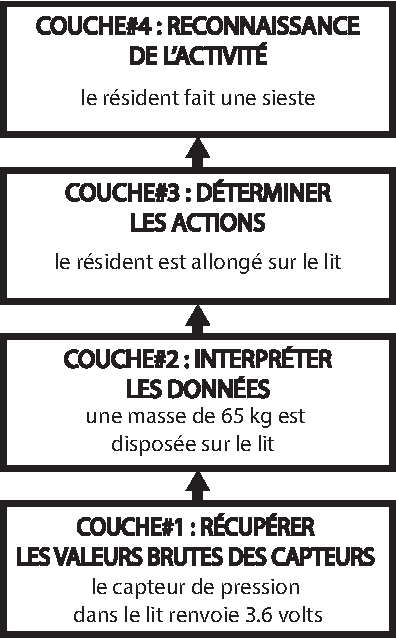
\includegraphics[width=5cm]{activity_recognition.pdf}
	\caption{Représentation multicouches de la reconnaissance d'activités dans les environnements intelligents.}
	\label{fig:activity_recognition}
\end{figure}

En définitive, il est donc possible d'effectuer une reconnaissance d'activités au sein d'un environnement intelligent à partir de capteurs de bas niveau\textemdash à condition que les différentes problématiques énoncées précédemment soient respectées tout au long du processus.

\section{Les habitats intelligents et les \textit{wearable devices}}

Au cours des dix dernières années, de nombreux travaux concernant les environnements intelligents et plus particulièrement, les habitats intelligents ont vu le jour. Pour reconnaître les activités des résidents, ceux-ci ont adopté des architectures sensiblement identiques, où les valeurs des capteurs sont centralisées en une entité unique (un serveur) qui va, à elle seule, exécuter toutes les couches de la reconnaissance d’activités \citep{Bouchard2014, Hu2016}. Néanmoins, certaines distinctions demeurent entre ces différentes implémentations. Par exemple, le \ac{LIARA} \citep{Bouchard2014} et le Laboratoire de \ac{DOMUS} \citep{Giroux2009} représentent les habitats intelligents hérités du monde de l’industrie. Les autres implémentations d'habitats intelligents comme Gator-Tech \citep{Helal2005}, MavHome \citep{DJCook2003}, CASAS \citep{Cook2013} ou encore Amiqual4home \citep{Lago2017} reposent toutes, quant à elles, sur des architectures par composants. Cependant, ces habitats intelligents connaissent certaines limitations. En effet, bien que les architectures centralisées simplifient l'utilisation des algorithmes de reconnaissance d'activités, elles ont un impact significatif sur la fiabilité de fonctionnement du système de reconnaissance et donc sur la sécurité du résident qui occupe l'habitat. Bien que de nouveaux travaux essayent de répondre à cette problématique \citep{Cook2013, Plantevin2018}, les habitats intelligents restent également, encore très dispendieux.

Par ailleurs, les recherches réalisées dans la reconnaissance d'activités au sein d'un habitat intelligent se sont intéressées, en grande partie, à reconnaître les activités d'un unique habitant dans l'environnement (mono-résident) \cite{VikramadityaJakkula2007, VanKasteren2008, Inomata2009, Ghazvininejad2011, Belley2014, Fortin-Simard2015}. Bien que très performantes, ces solutions se sont retrouvées défaillantes lorsque l'habitat est occupé par plusieurs résidents (multi-résident). Ce cas de figure constitue pourtant une problématique bien plus proche de la réalité actuelle des habitats intelligents. De nouvelles techniques de reconnaissance d'activités ont donc été proposées \citep{Crandall2009, Cook2009, Alemdar2013, Ayuningtyas2014, Emi2015, Mokhtari2018}. Plusieurs d'entre elles \citep{Mihailidis2004, Tunca2014} se sont alors tournées vers l'utilisation de \textit{wearable devices}, beaucoup plus accessibles financièrement. D'autre part, grâce à la miniaturisation de ces appareils, ceux-ci tendent à être de moins en moins considérés comme intrusifs par leur utilisateurs \citep{Gaskin2017}. En plus de la reconnaissance d'activités mono-résident et multi-résidents, ces capteurs portables ont permis l'ouverture de nouveaux horizons de recherche et ont principalement été utilisé pour la surveillance de la santé, la réhabilitation physique, la détection de chutes, \textit{etc.} \citep{Patel2012, Mukhopadhyay2014, Delahoz2014}. 

L'augmentation de l'utilisation des \textit{wearable devices} au sein des habitats intelligents a fait émerger de nouvelles problématiques. Dans un premier temps, puisque ceux-ci se trouvent placés au plus près des résidents, il devient alors possible d'envisager de nouveaux types de reconnaissance permettant d'améliorer la qualité de l'assistance proposée. Néanmoins, puisque les différentes architectures recensées dans la littérature n'ont pas été initialement prévues pour accueillir ce type de matériel, les \textit{wearable devices} se retrouvent très mal, voir nullement intégrés à celles-ci. Il apparaît donc primordial de s'intéresser à une manière de mieux les intégrer, dans le but de proposer un processus de reconnaissance combinée entre les données fournies, à la fois par les capteurs ambiants et portables, ce qui apparaît difficilement faisable actuellement tant en termes d'intégration matérielle que d'exploitation logicielle. En effet, les dispositifs actuels exploitent uniquement les données qu'ils génèrent eux-mêmes, mais il apparaît crucial de proposer une solution afin de pouvoir utiliser, de manière générique, les données générées par plusieurs \textit{wearable devices}.

\section{Définition du projet de recherche}
\label{sec:def_proj}
Ce projet de thèse s'articule donc autour de l'exploitation des \textit{wearable devices} ainsi que de l'interopérabilité de ces derniers avec l'utilisation de l'intelligence ambiante au sein des habitats intelligents. Plus particulièrement, ce projet de thèse permettra de répondre aux questions suivantes : 

\begin{enumerate}
	\item 
		\label{question:1}
		Quels nouveaux apports, en matière d'intelligence, les \textit{wearable devices} vont permettre de proposer aux résidents des habitats intelligents afin d'améliorer l'assistance qui leur est requise ?

	\item 
		\label{question:2}
		Comment optimiser l'intégration des \textit{wearable devices} afin qu'ils puissent être utilisés en combinaison avec les capteurs statiques présents dans les habitats intelligents pour réaliser une reconnaissance basée sur l'interopérabilité de ces deux méthodes ?
	
	\item 
		\label{question:3}
		Comment valoriser la réutilisation des différents algorithmes employés dans la reconnaissance d'activités avec les \textit{wearable devices} afin de faciliter les expérimentations dans un cadre académique ?
\end{enumerate}

Tout d'abord, différents \textit{wearable devices} permettant de réaliser de nouveaux types de reconnaissances seront développés afin de proposer une meilleure assistance aux résidents de l'habitat intelligents. Ensuite, l'objectif de ce projet de thèse est de mettre en place un framework pour faciliter l'intégration des \textit{wearable devices} au sein des ces environnements. Celui-ci fournira une couche d'abstraction autant envers l'architecture de l'habitat dans lequel il est déployé qu'envers le dispositif lui-même. Enfin, cet outil aura également pour fonction de faciliter l'utilisation de ces appareils, dans un cadre académique, en offrant la possibilité de valider plus rapidement le fonctionnement des prototypes.

\section{Organisation du document}

Le reste de ce projet de thèse se découpe en trois chapitres. Le \autoref{chap:2} va, dans un premier temps, présenter les différentes architectures d'habitats intelligents existantes. Dans un second temps, ce chapitre expliquera plus en détail le processus de reconnaissance d'activité et plus spécifiquement, les différents algorithmes qui sont utilisés pour l'apprentissage et la classification. Ensuite, le \autoref{chap:3} explicitera le fonctionnement des \textit{wearable devices} ainsi que les différentes applications de ceux-ci au sein des habitats intelligents. Enfin le \autoref{chap:4}, quant à lui, est dédié à la présentation de la méthodologie mise en place pour parvenir aux objectifs de ce projet de thèse ainsi que la planification des jalons nécessaires jusqu'en décembre 2019.
\let\cleardoublepage\clearpage
\chapter{L'Intelligence Ambiante au sein des habitats intelligents}
\label{chap:2}

Dans le chapitre précédent, la reconnaissance d'activité a été définie et son application concrète au sein d'environnements intelligents a été brièvement abordée. Néanmoins, avant d'entrer plus en détail sur le fonctionnement du processus de la reconnaissance d'activité, il convient d'étudier les différents types d'environnements dans lesquels elle est appliquée. Ainsi, ce chapitre va, dans un premier temps, présenter l'état de l'art des différents types d'architectures existantes pour enfin, proposer une étude détaillée du processus de la reconnaissance d'activités. Cette dernière partie présentera notamment l'ensemble des étapes nécessaires pour y parvenir ainsi que les différents algorithmes utilisés.

\section{Les habitats intelligents existants}

Dans la dernière décennie, plusieurs implémentations d'habitats intelligents, visant à mettre en pratique le concept de reconnaissance d'activités multicouche tel que présenté par \cite{Roy2013}, ont émergé \citep{DJCook2003, Helal2005, Giroux2009, Cook2013, Bouchard2014, Lago2017}. Néanmoins, en l'absence de toute spécification formelle d'une architecture optimale pour ces habitats, chacune des applications proposées demeure différente malgré leur motivation commune. Puisque l'un des objectifs de ce projet de thèse est de proposer une meilleure intégration des \textit{wearable devices} au sein des habitats intelligents\textemdash il convient d'identifier les réelles différences entre ces architectures afin d'en extraire leurs avantages et leurs inconvénients. Pour ce faire, cette première partie se découpe en trois sous-sections qui correspondent chacune à un type d'implémentation parmi les plus avancées dans le domaine soit, les architectures industrielles avec le \acs{LIARA} \citep{Bouchard2014} et le \acs{DOMUS} \citep{Giroux2009}, les architectures basées composants avec MavHome \citep{DJCook2003}, Gator-Tech \citep{Helal2005} et Amiqual4home \citep{Lago2017} et enfin CASAS \citep{Cook2013}, l'habitat intelligent qui repose sur un réseau maillé ZigBee. Cependant, ce projet de thèse ne tient pas compte des habitats intelligents qui reposent sur l'utilisation de technologies considérées trop intrusives pour reconnaître les activités de leurs résidents, comme les caméras ou les microphones \citep{Brumitt2000, Vacher2011}.

\subsection{Le \acs{LIARA} et le laboratoire \acs{DOMUS}}

Le \acs{LIARA} \citep{Bouchard2014} et le Laboratoire \acs{DOMUS} \citep{Giroux2009} sont deux environnements académiques de recherche pour la reconnaissance d'activités. Ces deux laboratoires disposent d'habitats intelligents qui reposent sur des technologies héritées du milieu industriel. Comme illustré en figure \ref{fig:archi_liara_domus}, leur architecture s'articule essentiellement autour d'une entité de calcul centrale (le serveur) ainsi qu'un automate industriel qui permet de récupérer les valeurs des différents capteurs qui sont divisés en îlots. Ces valeurs sont ensuite enregistrées dans une base de données de type relationnelle. Ainsi, les couches supérieures de la reconnaissance d'activités peuvent être réalisées sur le serveur par le biais d'une unique interface.

\begin{figure}[H]
	\centering
	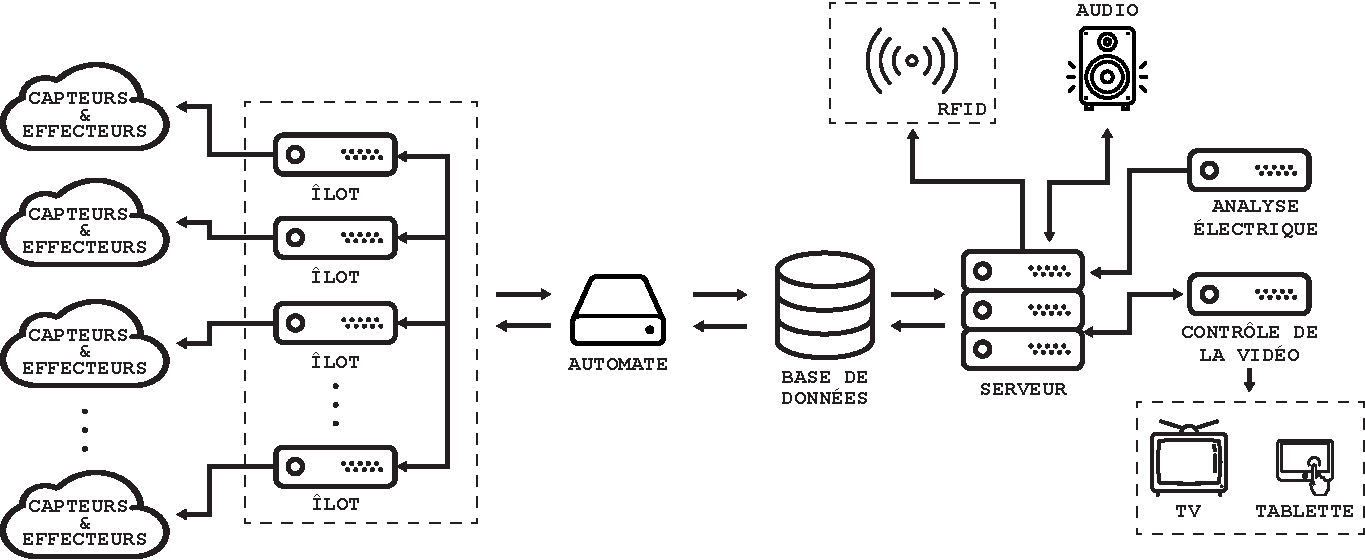
\includegraphics[width=\linewidth]{archi_liara_domus.pdf}
	\caption{Schématisation de l'architecture utilisée par le \acs{LIARA} et le laboratoire \acs{DOMUS}.}
	\label{fig:archi_liara_domus}
\end{figure}

Le principal avantage d'une telle architecture concerne l'exploitation d'un matériel industriel directement. En effet, ce dernier étant conçu pour fonctionner sans interruption dans des environnements stressants comme des usines, il demeure extrêmement robuste et fiable sur le long terme. Cela permet donc de garantir la qualité de fabrication pour l'habitat intelligent. Aussi, le choix d'une architecture centralisée favorise un accès simplifié aux données de l'habitat. La couche matérielle est abstraite pour les différents programmes de reconnaissance et d'assistance qui peuvent alors interroger directement la base de données. 

Malgré ces avantages, une architecture comme celle du \acs{LIARA} et du laboratoire \acs{DOMUS} présentent des inconvénients majeurs. Le premier concerne le coût global. En effet, \cite{Plantevin2018a} a évalué le prix de ces habitats à 13 500 dollars US sans compter les capteurs, les effecteurs, l'installation et le support. Un investissement de cette ampleur est donc conséquent pour les personnes en perte d'autonomie, car dans une grande majorité, ceux-ci vivent dans des conditions financières précaires, et ce, malgré la prise en charge de certains frais par leur régime d'assurance \citep{AlzheimersAssociation2018}. De plus, bien que le matériel industriel soit un gage de qualité de l'habitat, il n'est pas impossible qu'une panne survienne, par exemple la perte d'un îlot, de l'automate ou du serveur. De ce fait, puisque l'architecture est centralisée, le fonctionnement de l'habitat peut être partiellement ou totalement altéré. Dans le pire des cas, l'assistance au résident devient donc impossible et des situations dangereuses pour sa sécurité peuvent survenir. Finalement, une architecture monolithique telle que celle-ci ne facilite pas l'intégration de nouveaux capteurs qui doivent être ajoutés manuellement dans le système. De plus, l'intégration de capteurs qui ne peuvent être reliés par câble aux îlots de l'habitat demeure extrêmement complexe \citep{Plantevin2018a}. Il apparaît donc clairement que l'évolutivité de l'architecture ainsi que l'utilisation de \textit{wearable devices} n'ont pas été pris en compte lors de la conception de cette architecture.

\subsection{MavHome, Gator-Tech et Amiqual4home}

Pour répondre à la problématique de l'évolutivité, des architectures basées composant ont été développées. Le premier exemple d'habitat intelligent exploitant ce type d'architecture est MavHome \citep{DJCook2003}. Cette dernière repose sur une interface \ac{CORBA}\footnote{\url{www.corba.org}} permettant la liaison entre les différents composants logiciels et le contrôleur électrique des appareils présents dans l'habitat. Cependant, en raison de la complexité des contraintes imposées par ce standard, des solutions plus récentes comme Gator-Tech \citep{Helal2005}, Amiqual4home \citep{Lago2017} ou encore les initiatives proposées par \cite{Novak2011} et \cite{Cheng2012} ont préféré l'emploi de la technologie \ac{OSGi}. Tous ces habitats partagent des caractéristiques identiques. Par conséquent, seuls les cas de Gator-Tech et d'Amiqual4home seront détaillés dans cette section, car ils reviennent fréquemment dans la littérature.

L'habitat Gator-Tech a pour objectif de répondre à une problématique des habitats de type industriel, à savoir la simplification du processus d'intégration de nouveaux capteurs. Pour ce faire, son architecture repose essentiellement sur la technologie \acs{OSGi}\footnote{\url{www.osgi.org/developer/architecture}}. Comme illustré par la figure \ref{fig:archi_gator_tech}, chaque capteur de l'habitat possède son propre pilote qui va lui permettre de communiquer avec l'intégralité du système. Ce pilote est stocké dans une mémoire morte dans le but de conserver les données, même lorsque le matériel n'est pas alimenté. Ainsi, lors de la mise en fonction d'un capteur, celui-ci s'enregistre de manière autonome auprès d'une définition de service. Cette dernière va alors servir de couche d'abstraction pour la création de services de base qui peuvent soit permettre de consommer des données fortement abstraites, soit être combinés afin d'obtenir un service composite. Un service de base peut, par exemple, renvoyer \textit{``la plaque de cuisson est chaude''} lorsque la sonde de température de la cuisinière donne une valeur supérieure à 50\textdegree{}C ; alors qu'un service composite peut, quant à lui, agréger tous les services basiques des capteurs \ac{RFID} pour localiser un résident dans l'habitat. De ce fait, il est possible de concevoir des programmes de reconnaissance et d'assistance sans jamais se préoccuper du protocole de communication des capteurs, ni du format dans lequel ils transmettent les données.

Ce même fonctionnement est utilisé par l'habitat intelligent Amiqual4home. Cet environnement s'appuie sur \ac{openHAB}\footnote{\url{www.openhab.org}}, un \textit{middleware open source} dédié aux habitats intelligents, qui s'appuie sur un environnement \acs{OSGi} ainsi que sur le \textit{framework} Eclipse SmartHome\footnote{\url{www.eclipse.org/smarthome}} spécifiquement conçu pour fonctionner dans cet environnement. Ainsi, comme illustré par la figure \ref{fig:archi_amiqual4home}, \acs{openHAB} permet de créer une couche d'abstraction autour des couches service, connaissance et logicielle visibles sur la figure \ref{fig:archi_gator_tech}.

\begin{figure}
	\centering
	\subfloat[Gator-Tech]{
		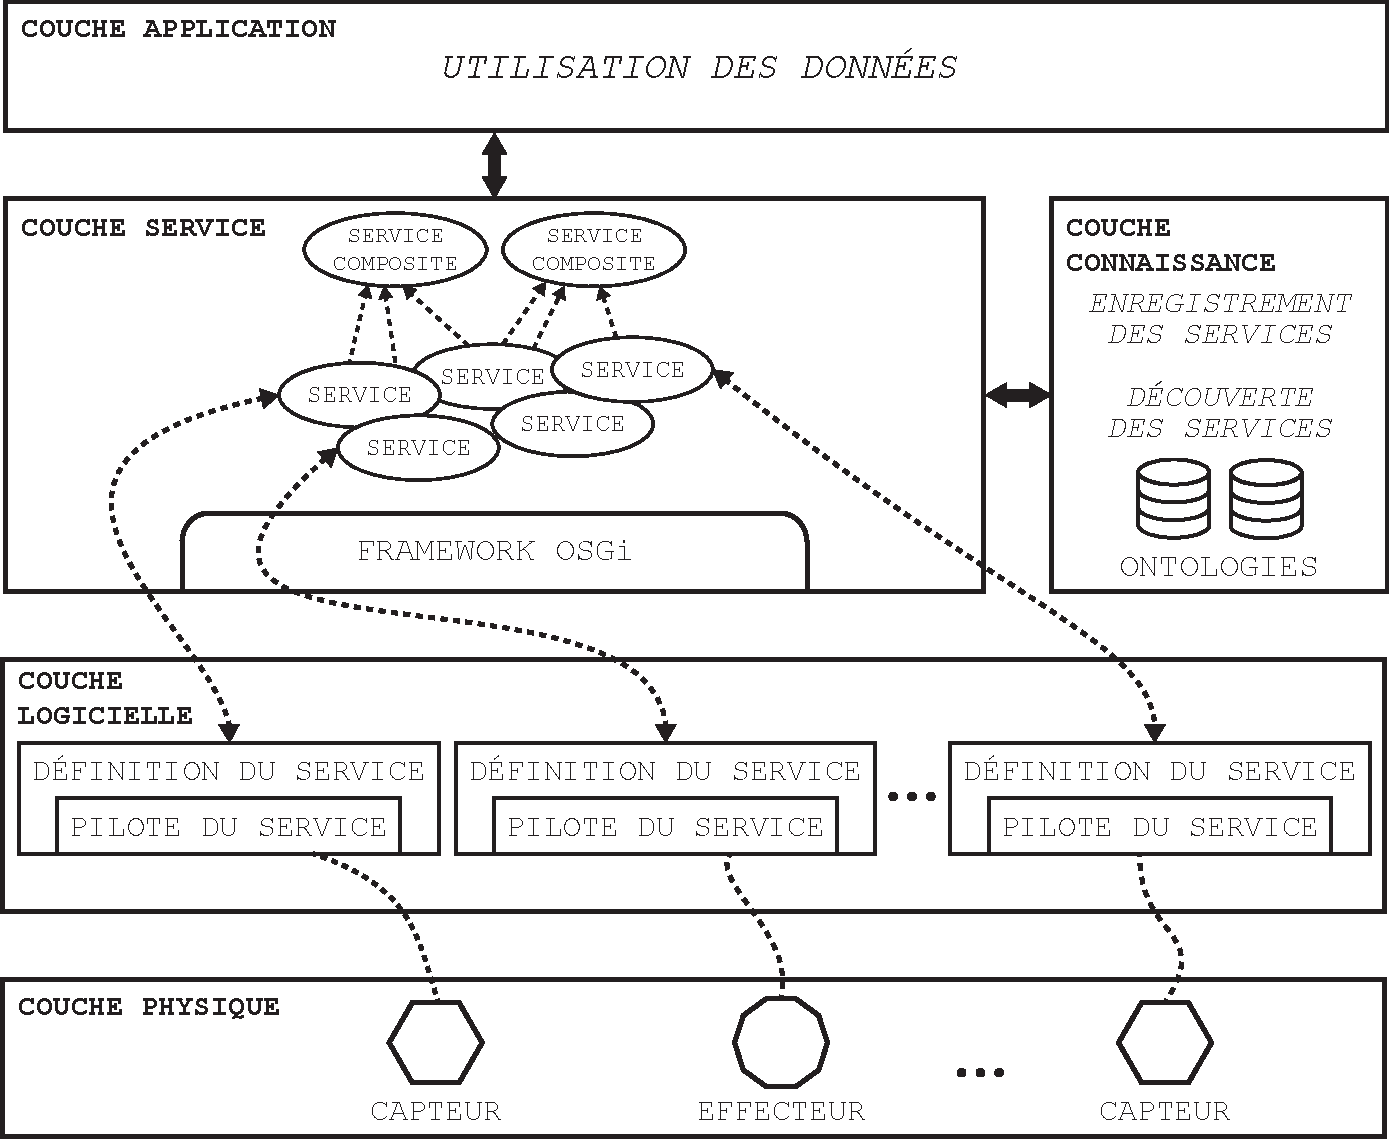
\includegraphics[width=.8\linewidth]{archi_gator_tech.pdf}
		\label{fig:archi_gator_tech}
	}
	\\[20pt]
	\subfloat[Amiqual4home]{
		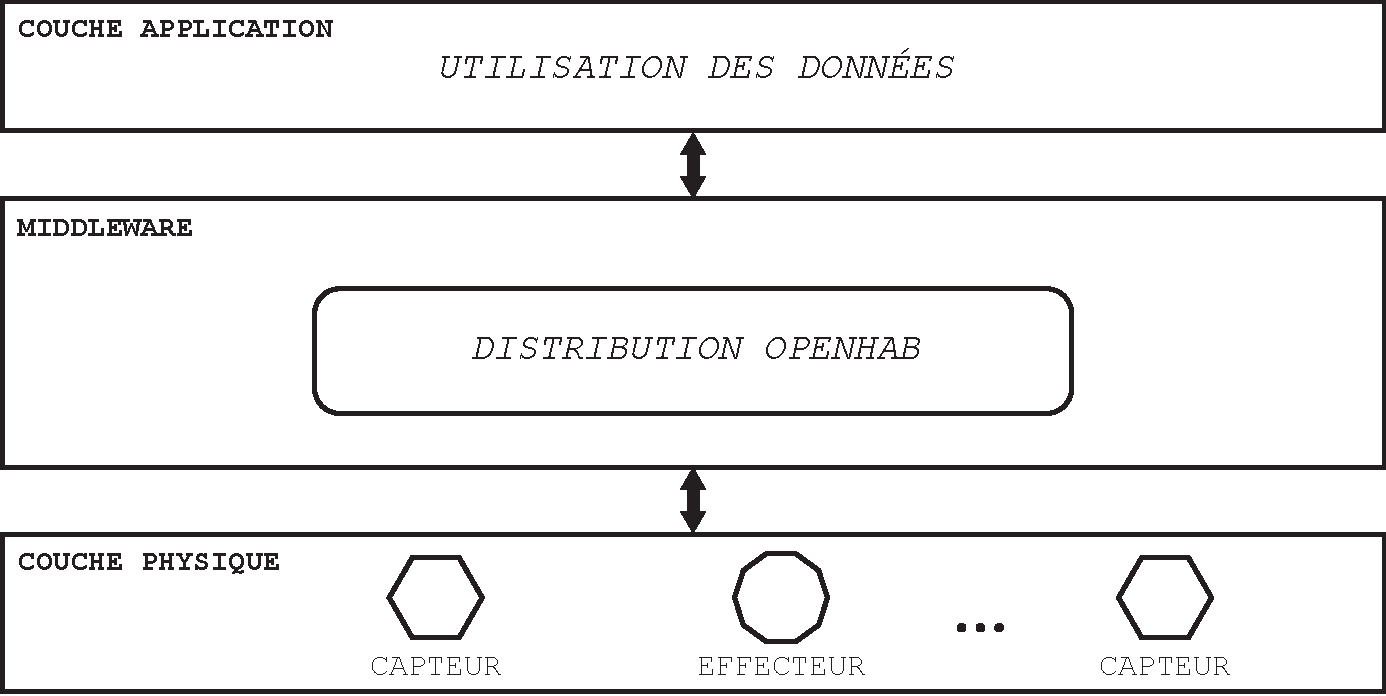
\includegraphics[width=.8\linewidth]{archi_amiqual4home.pdf}
		\label{fig:archi_amiqual4home}
	}
	\caption{Schématisation des architectures utilisées par les habitats Gator-Tech et Amiqual4home}
\end{figure}

Le principal avantage de ce type d'architectures est qu'elles supportent parfaitement la mise à l'échelle de l'environnement dans le cas d'ajouts ou de remplacements de capteurs. Il semble également que l'intégration de \textit{wearable devices} soit possible, sans effort particulier, grâce à la flexibilité offerte par les architectures basées composants. De plus, l'exploitation de données fortement abstraites facilite le développement de programmes de reconnaissance et d'assistance, puisqu'un raisonnement sur ce type de données demeure plus simple que d'exploiter les données brutes directement \citep{Helal2005}. Enfin, il est possible que le coût d'un tel habitat soit considérablement réduit en comparaison à un habitat basé sur une architecture industrielle. En effet, dans le cas de Gator-Tech, son architecture requiert toujours un serveur central. Néanmoins, elle n'implique pas l'utilisation d'un automate ou d'îlots, et les capteurs utilisés au sein de cet environnement sont basés sur des plateformes à faible coût \citep{Helal2005}. Cependant, tout comme pour les habitats de type industriels, Gator-Tech et les autres architectures basées composant souffrent du même inconvénient majeur, c'est-à-dire, le recourt à un serveur central comme seule unité de calcul. Dans le cas présent, ce dernier provoque la création d'un goulot d'étranglement. En effet, un large flux de données qui transitent par le serveur peut entraîner un ralentissement de celui-ci. Il devient alors surchargé et l'assistance pour le résident n'est plus réalisée convenablement.

\subsection{CASAS}

Récemment, grâce aux avancements des technologies de communication sans-fil, de nouveaux types d'habitats intelligents ont émergé. Ainsi, il est notamment possible d'en retrouver plusieurs dont l'architecture s'articule autour d'un réseau maillé ZigBee comme CASAS \citep{Cook2013}, ou encore les initiatives proposées par \cite{Zhihua2016} et \cite{Zhenyu2011}. Bien qu'ils admettent des différences, ces trois habitats demeurent sensiblement identiques dans la conception de l'architecture qu'ils proposent. De ce fait, cette section ne traite exclusivement du cas de CASAS, puisque celui-ci reste le plus connus d'entre eux. En introduisant CASAS, \cite{Cook2013} voulaient principalement résoudre le problème du coût que représentent les habitats intelligents, mais également en faciliter leur installation. C'est ainsi que le concept d'habitat intelligent en boîte est né. Comme montré par la figure \ref{fig:archi_casas}, l'architecture de CASAS se décompose en quatre composants principaux. Tout d'abord, il y a la couche physique qui contient le réseau maillé ZigBee. Dans le cas de cet habitat, il s'agit d'une topologie de réseau sans-fil où tous les n\oe{}uds, c'est-à-dire les capteurs et les effecteurs, sont connectés pair à pair et collaborent pour s'échanger des données. Le réseau maillé communique ensuite avec un service de messagerie au travers un pont ZigBee. Ce dernier a pour but de transformer les données des capteurs en messages \ac{XMPP} de plus haut niveau. Le service de messagerie étant de type \textit{publish/subscribe}, il offre alors la possibilité à d'autres services de s'y connecter. C'est notamment le cas du service d'archivage. Ce dernier récupère, par l'intermédiaire du pont scribe, certains évènements qui se produisent dans l'habitat afin de les enregistrer dans une base de données d'archives. Finalement, les applications de reconnaissance et d'assistance exploitent les données du \textit{middleware} en les récupérant \textit{via} le pont applicatif. 

\begin{figure}[H]
	\centering
	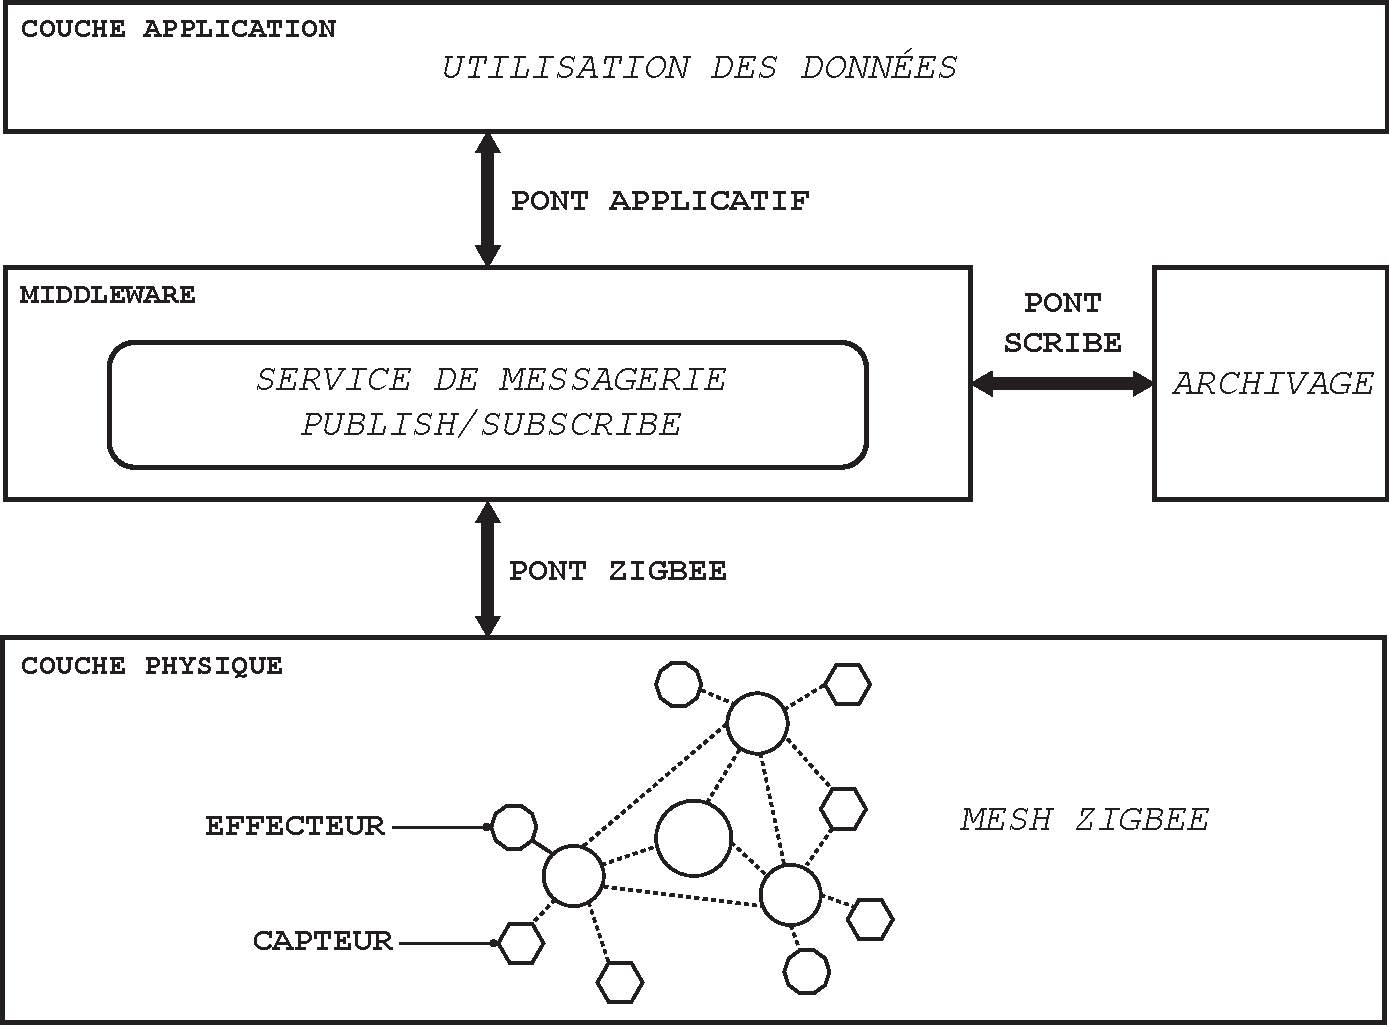
\includegraphics[width=.8\linewidth]{archi_casas.pdf}
	\caption{Schématisation de l'architecture utilisée par l'habitat CASAS.}
	\label{fig:archi_casas}
\end{figure}

Les habitats intelligents basés sur les réseaux maillés ZigBee sont des solutions réellement moins onéreuses que les autres types d'architectures d'habitats. En effet, \cite{Cook2013} rapportent un coût total estimé à 2 765 dollars US, soit presque 5 fois moins qu'un habitat industriel. Par ailleurs, puisque les habitats basés sur un réseaux maillé reposent tous sur la technologie de communication sans-fil ZigBee, il semble relativement aisé d'y ajouter de nouveaux capteurs et notamment d'y intégrer des \textit{wearable devices}. Cependant, l'inconvénient majeur du protocole ZigBee est que les signaux ne sont pas directement compatibles avec des systèmes évolués tels que les ordinateurs ou les téléphones intelligents. De plus, tous les \textit{wearable devices} ne disposent pas toujours d'une connectivité ZigBee. En effet, la grande majorité d'entre eux ont plutôt adopté la technologie \ac{BLE} \citep{Martin2014}, qui est également devenue compatible avec la topologie réseau maillé récemment \citep{Bluetooth2017}. 

Il apparaît donc clairement qu'une architecture adaptative quant à l'intégration des \textit{wearable devices} est nécessaire. Bien que les architectures basées sur un réseau maillé constituent un premier pas en ce sens, la variété des technologies de communication et des protocoles qu'elles peuvent exploitées n'est pas encore pleinement prise en compte dans leur conception. 

\section{Le processus d'apprentissage pour reconnaître des activités}

Le processus d'apprentissage pour la reconnaissance d'activités est un ensemble d'étapes qu'il est généralement possible de réaliser pour reconnaître des activités. Tel qu'illustré par la figure \ref{fig:ar_process}, ce processus requiert des données initiales fournies par les capteurs ambiants ou portables. Celles-ci n'ont alors été soumises à aucun traitement en particulier, ce sont donc des données brutes. Principalement en fonction de la condition des capteurs et de la transmission des valeurs, les données obtenues peuvent se retrouver altérées. Afin d'améliorer leur qualité, il est donc possible, dans un second temps, d'effectuer une étape de prétraitement. Ensuite, puisque les données renvoyées représentent un signal ayant une longueur potentiellement infinie, il est impératif de segmenter ce dernier en plusieurs fragments, sur chacun desquels, des propriétés discriminantes sont calculées. L'ensemble de celles-ci, une fois extraites, constitue alors une abstraction du fragment traité. Le signal fragmenté est donc réduit à un unique vecteur de caractéristiques pour chaque segment. Dans certains cas, il peut s'avérer que celui-ci contienne un nombre de propriétés suffisant pour impacter négativement la performance de la reconnaissance\textemdash auquel cas, une étape supplémentaire pour réduire la dimensionnalité du vecteur est requise. Cet ensemble de données est ensuite utilisé comme entrée d'un algorithme d'apprentissage qui, pour chacun des vecteurs réduits, retournera les noms des classes associées aux activités à reconnaître. Finalement, la dernière étape du processus consiste en une évaluation de la performance de la reconnaissance.

\begin{figure}[H]
	\centering
	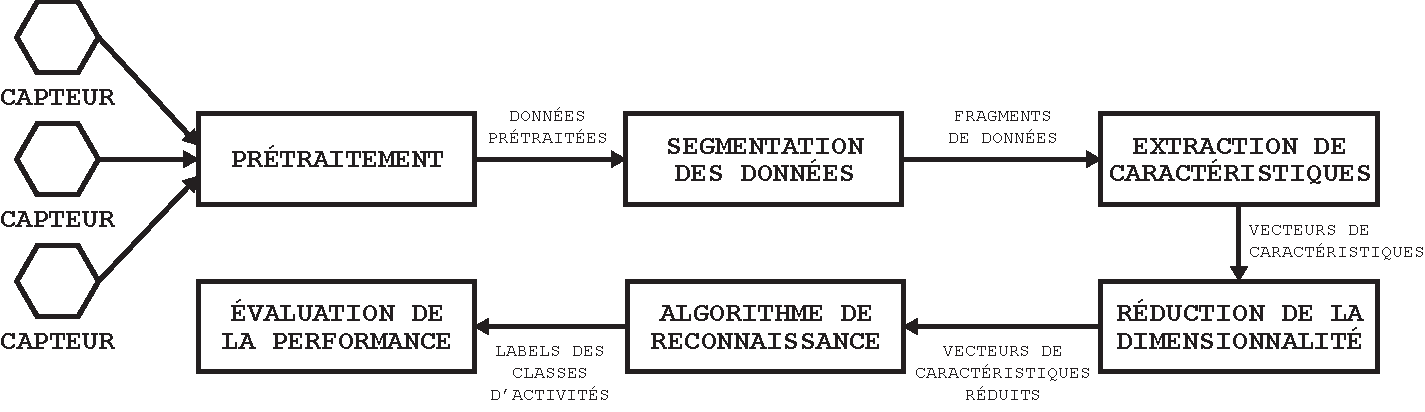
\includegraphics[width=\linewidth]{ar_process.pdf}
	\caption{Schématisation du processus d'apprentissage pour la reconnaissance d'activités.}
	\label{fig:ar_process}
\end{figure}

\subsection{Les étapes préliminaires}

Avant d'être utilisées par l'algorithme d'apprentissage, les données brutes issues des capteurs passent par un ensemble d'étapes préliminaires afin d'être transformées en caractéristiques discriminantes. Ainsi, cette section va présenter les méthodes les plus utilisées en ce qui concerne le prétraitement et la segmentation des données, mais également l'extraction de caractéristiques et la réduction du nombre qui en est produit, c'est-à-dire la réduction de la dimensionnalité. 

\subsubsection{Prétraitement des données}

Le prétraitement des données est la première étape du processus d'apprentissage pour la reconnaissance d'activités. En effet, après l'acquisition des valeurs renvoyées, autant par les capteurs ambiants que les capteurs portables présents au sein d'un environnement intelligent, plusieurs facteurs peuvent influer sur la qualité de ces données. Par exemple, un mauvais fonctionnement du matériel ou un problème de transmission comme une latence réseau peuvent entraîner l'acquisition de données incohérentes, erronées ou encore partiellement manquantes. Les objectifs de cette étape sont donc d'améliorer les données récoltées en réduisant le bruit, ou en filtrant les éléments nuisibles, tout en essayant de conserver les caractéristiques dynamiques essentielles du signal. 

Dans le cas où les données comprendraient des valeurs partiellement manquantes, plusieurs méthodes peuvent être employées pour pallier cette perte. Dans un premier temps, il est tout simplement possible d'ignorer les données incriminées. Néanmoins, cette méthode n'est pas pertinente lorsque l'absence d'information est très élevée. De ce fait, il est possible de remplacer les valeurs manquantes pour un attribut donné grâce à une estimation qui peut être déterminée selon deux procédés différents. Le premier consiste à calculer la moyenne de toutes les valeurs non manquantes pour l'attribut en question. La seconde méthode implique que les données soient labélisées et consiste à remplacer la valeur manquante d'un attribut par la moyenne des valeurs présentes qui appartiennent à la même classe celui-ci. 

De plus, il est admis que les capteurs \ac{RFID} et les accéléromètres sont connus pour être les deux types de capteurs (ambiant et portable) les plus sujets au bruit. Or, de nombreux travaux se basent sur l'exploitation de ceux-ci dans le but de reconnaître des activités \citep{Ravi2005, Stikic2008, Buettner2009, Khan2011, Mannini2017}. De ce fait, \cite{Wang2011} ont comparé quatre filtres différents ayant pour but de réduire le bruit dans les données générées par un accéléromètre, soit : un filtre médian \citep{Huang1979}, un filtre passe-bas de type \textit{Butterworth} \citep{Butterworth1930}, une transformée en ondelettes discrète spécifique (\ac{DWPD}) \citep{Mallat1989} et un filtre de Kalman \citep{Welch2006}, où ce dernier s'est révélé comme le plus efficace. \cite{Abreu2014} ont, quant à eux, montré que le filtre de Kalman était également le plus performant pour réduire le bruit présent dans le leur système de localisation intérieure basé sur des capteurs \acs{RFID}.

\subsubsection{Segmentation des données}

Dans le processus d'apprentissage, la segmentation des données peut intervenir, soit après la première phase de prétraitement, soit directement sur les données brutes si celles-ci ne sont pas altérées. Cette opération consiste à découper un signal donné en plusieurs fragments plus petits. En d'autres termes, le signal est morcelé en une séquence de segments qui sont délimités par un temps de départ et un temps d'arrivée. Du point de vue du traitement de signal, cette opération est appelée le fenêtrage. Ainsi, il est possible d'observer le signal d'origine $x\left(t\right)$ de longueur théoriquement infinie, sur une durée finie $T$ en le multipliant par une fonction fenêtre d'observation $w\left(t\right)$ tel que,

% Dans le processus d'apprentissage, la segmentation des données peut intervenir, soit après la première phase de prétraitement, soit directement sur les données brutes si celles-ci ne sont pas altérées. Cette opération consiste à découper un signal donné $X$ en plusieurs fragments plus petits $x_i$. Chaque segment $x_i = (T_1, T_2)$ est alors délimité par un temps de départ $T_1$ et un temps d'arrivée $T_2$. Le signal est donc morcelé en une séquence de segments tel que,

% \begin{equation}
%     X = \left\{x_n\right\}, \quad n \in \mathbb{N} .
% \end{equation}

% \noindent Du point de vue du traitement de signal, cette opération est appelée le fenêtrage. Ainsi, il est possible d'observer le signal d'origine $x\left(t\right)$ de longueur théoriquement infinie, sur une durée finie $T$ en le multipliant par une fonction fenêtre d'observation $w\left(t\right)$ tel que,

\begin{equation}
    x_w\left(t\right) = x\left(t\right)w\left(t\right), \quad 0 \leq t \leq T - 1 .
\end{equation}

En ce qui concerne la reconnaissance d'activités, il est possible de regrouper les techniques de segmentation en trois groupes distincts : la segmentation basée sur les activités, la segmentation basée sur des évènements et la segmentation par fenêtre glissante \citep{Banos2014}. 

La segmentation basée sur les activités revient à partitionner le signal selon la détection d'un changement significatif correspondant à une activité. Un tel découpage peut-être réalisé grâce à l'analyse du domaine fréquentiel du signal ou de son énergie \citep{Sekine2000, Guenterberg2009}.

La segmentation basée sur les évènements exploite, quant à elle, un découpage du signal selon la manifestation d'évènements spécifiques. Par exemple, cette méthode est souvent utilisée dans la reconnaissance de la marche ou d'autres activités similaires comme courir, monter ou descendre des escaliers, \textit{etc. } Puisque ces activités sont cycliques et requièrent des actions inévitables (\textit{p. ex., } le contact du pied sur le sol), il est possible de segmenter le signal par l'analyse de l'accélération \citep{SantAnna2010}, mais également en exploitant d'autres types de données comme celles issues de capteurs de pression \citep{Crea2012}. 

Enfin, la segmentation par fenêtre glissante peut se traduire comme étant la translation d'une fenêtre sur l'axe temporel du signal, où chaque déplacement de la fenêtre représente un segment. Une fenêtre est définie par une fonction mathématique, une taille ainsi qu'un pourcentage de superposition. En ce qui concerne ce dernier, si une fenêtre est définie comme ayant une taille de 100 secondes avec un pourcentage de superposition de 50\%, le premier intervalle sera $\left[0,100\right]$ tandis que le second sera $\left[50,150\right]$ et ainsi de suite. Parmi les fonctions de fenêtrage les plus fréquemment utilisées, il est possible de mentionner, la fenêtre de Hamming, celle de Kaiser, de Hann ou encore la fenêtre de Blackman respectivement exprimées par :

\begin{equation}
	\label{eq:Hamming}
	w\left(t\right) = \left\{
	\begin{array}{ll}
		0.54-0.46\cos(\frac{2\pi t}{T-1}), & \mbox{si } 0 \leq t \leq T-1 \\
		0,								   & \mbox{sinon.}
	\end{array}
	\right.
\end{equation}

\begin{equation}
	\label{eq:Kaiser}
	w\left(t\right) = \left\{
	\begin{array}{ll}
		\frac{I_0\left[\alpha\sqrt{1-(\frac{2t}{T-1}-1)^2}\,\right]}{I_0\left[\alpha\right]}, & \mbox{si } 0 \leq t \leq T-1 \\
		0,                                    & \mbox{sinon.}
	\end{array}
	\right.
\end{equation}

\begin{equation}
	\label{eq:Hann}
	w\left(t\right) = \left\{
	\begin{array}{ll}
		0.5-0.5\cos(\frac{2\pi t}{T-1}), & \mbox{si } 0 \leq t \leq T-1 \\
		0, & \mbox{sinon.}
	\end{array}
	\right.
\end{equation}

\begin{equation}
	\label{eq:Blackman}
	w\left(t\right) = \left\{
	\begin{array}{ll}
		0.42-0.5\cos(\frac{2\pi t}{T-1}) + 0.08\cos(\frac{4\pi t}{T-1}), & \mbox{si } 0 \leq t \leq T-1 \\
		0,                                    & \mbox{sinon.}
	\end{array}
	\right.
\end{equation}

\noindent où, $I_0 $ est la fonction de Bessel modifiée d’ordre zéro, $\alpha$ est le paramètre réel non nul caractérisant la forme de la fenêtre et $T$ est la taille de la fenêtre. Néanmoins, tous les paramètres impliqués dans le processus de la segmentation doivent être déterminés en fonction de la problématique, où l'objectif est de trouver le meilleur compromis entre la rapidité d'exécution et la performance de reconnaissance \citep{Banos2014}. 

\subsubsection{Extraction de caractéristiques}

L'extraction de caractéristiques est une phase importante dans le processus d'apprentissage pour reconnaître des activités. L'objectif de cette opération consiste à produire un vecteur de caractéristiques discriminantes pour chaque fragment du signal généré, grâce à un certain nombre de fonctions mathématiques. Il existe deux principaux domaines auxquels appartiennent les différentes techniques d'extraction : le domaine temporel et le domaine fréquentiel \citep{Huynh2005, Figo2010, Cleland2013a}. Les caractéristiques issues du domaine temporel demeurent les plus simples à obtenir. Il est notamment possible d'y retrouver des métriques statistiques comme la moyenne, la variance, l'écart type, l'asymétrie ou encore le kurtosis (la courbure) du signal, mais également des métriques dites \og enveloppe \fg comme la médiane, le minimum ou le maximum du signal. De plus, de nombreuses autres métriques temporelles peuvent être utilisées dans la reconnaissance d'activités, comme la corrélation entre deux signaux ou encore le \textit{zero crossing rate}\textemdash qui correspond au taux de changement de signe d'un signal. Les formules de l'asymétrie $S$, du kurtosis $K$ et de la corrélation $\rho$ de deux signaux $n \mbox{ et } n'$ sont respectivement données par : 

\begin{equation}
	S \left(n\right) = \frac{N}{(N-1)(N-2)} \cdot \left(\sum_{i=1}^{N}{\frac{(n_i-\bar{n})^3}{\sigma_n^3}}\right)
\end{equation}

\begin{equation}
	K \left(n\right) = \frac{N(N+1)}{(N-1)(N-2)(N-3)} \cdot \left(\sum_{i=1}^{N}{\frac{(n_i-\bar{n})^4}{\sigma_n^4}-\frac{3(N-1)^2}{(N-2)(N-3)}}\right)
\end{equation}

\begin{equation}
	\rho\left(n, n^{\prime}\right) = \frac{cov\left(n, n^{\prime}\right)}{\sigma_n\cdot\sigma_{n^{\prime}}}
\end{equation}

\noindent où $N$ représente la taille d'un fragment du signal, $n_i$ est le $i^{\grave{e}me}$ élément du fragment, $\bar{n}$ est la valeur moyenne du fragment et $\sigma_n$ correspond à l'écart type du fragment.

D'autre part, afin d'exploiter des caractéristiques issues du domaine fréquentiel, il est nécessaire de réaliser un passage vers celui-ci, depuis le domaine temporel. Pour ce faire, il s'agit de calculer la transformée de Fourier discrète du signal. Dans la grande majorité des cas, c'est l'algorithme de la transformée de Fourier rapide (\acl{FFT} ou \acs{FFT}) qui est utilisé à cet effet \citep{Brigham1967}. Malgré sa popularité, il est également possible d'utiliser l'algorithme de Goertzel pour réaliser la transformation depuis le domaine temporel vers le domaine fréquentiel \citep{Sysel2012}. Dès lors, les caractéristiques fréquentielles qui peuvent être calculées sont, la composante continue (\textit{DC Component}), l'énergie spectrale $E$ et l'entropie $H$ tel que, 

\begin{equation}
	\label{eq:energy_spec}
	E = \frac{1}{N}\cdot\left(\sum_{i=1}^{N}\mid{}n_i\mid\right)
\end{equation}

\begin{equation}
	\label{eq:entropy}
	H = - \sum_{i=1}^{N}{P_i}\ln P_i
\end{equation}

\noindent où $n$ représente un vecteur de nombres complexes de taille $N$ issu de la \acs{FFT}, $n_i$ est le $i^{\grave{e}me}$ élément du vecteur et $P_i$ est la probabilité de $n_i$ donnée par l'équation suivante : 

\begin{equation}
	\label{eq:pi}
	 P_i = \frac{n_i}{N - E}
\end{equation}

En dernier lieu, \cite{Mitchell2013} ont proposé une méthode de reconnaissance d'activités qui repose sur l'analyse par ondelettes (\ac{DWT}). À l'inverse de la transformée de Fourier, cette technique permet d'obtenir des caractéristiques à la fois issues du domaine temporel et fréquentiel, par décomposition d'un signal en un ensemble de coefficients d'ondelettes.

\subsubsection{Réduction de la dimensionnalité}

La dernière étape préliminaire concerne la réduction de la dimensionnalité du vecteur de caractéristiques. Cette étape est importante dans la mesure où elle permet de sélectionner l'ensemble des valeurs qui vont être conservées pour pallier le \textit{fléau de la dimension} \citep{Bellman1957}. Ce phénomène intervient lorsque la taille du vecteur de caractéristiques croît de manière conséquente. Les données peuvent alors se retrouver isolées et deviennent éparses, ce qui a pour effet de dégrader l'efficacité de la reconnaissance d'activités. Ainsi, en réduisant la dimensionnalité de ces données, l'objectif est de conserver les caractéristiques pertinentes tout en minimisant la perte d'information. Bien que ce processus doit permettre une meilleure reconnaissance, l'exploitation d'un plus petit vecteur peut également induire un traitement postérieur plus rapide. 

Actuellement, il existe une quantité importante de techniques de réduction de dimensionnalité. Par conséquent, \cite{VanDerMaaten2009} ont proposé une taxonomie dans laquelle ils recensent l'ensemble des méthodes existantes. En premier lieu, il possible de retrouver des techniques de réduction de la dimensionnalité orientées sélection de caractéristiques qui reposent sur des évaluations statistiques des données comme, la covariance ou l'entropie. L'avantage majeur de ces méthodes réside dans leur simplicité de mise en {\oe}uvre. D'autre part, bien qu'elle demeure une technique plus complexe, l'analyse par composantes principales (\acl{PCA} ou \acs{PCA}), a souvent été utilisée dans le domaine de la reconnaissance d'activités \citep{He2009, Altun2010, Chen2012, Leightley2013}. Elle permet, en s'appuyant sur un modèle géométrique, de transformer des caractéristiques qui sont initialement corrélées en de nouvelles caractéristiques décorrélées les unes des autres, les composantes principales.% Soit plus formellement, si $X=\left[x_1, x_2,\dotsc{},x_n\right]^T$ est un vecteur colonne de $n$ valeurs aléatoires ayant une moyenne nulle, l'objectif de cette méthode est de trouver une matrice orthogonale $V$ de taille $n\times k$ tel que $k \leq n$. Ainsi, la projection réduite $X'=VX$ de taille $k$ permet de conserver le plus de variances de $X$ que possible. La matrice $V$ définit la direction principale de la projection où ses composants sont calculés en utilisant la décomposition de celle-ci en éléments propres $C=E\Lambda E^T$ grâce à la matrice de covariance $C=E(XX^T)$. Les vecteurs propres $\Lambda=diag(\lambda_1, \lambda_2,\dotsc{}, \lambda_n)$ déterminent alors la variance des composantes principales. Finalement, les composantes principales $X'=\left[x^{\prime}_1, x^{\prime}_2,\dotsc{},x^{\prime}_n\right]$ sont obtenues par projection des données d'origines dans les directions principales $X'=E^TX$ \citep{Jolliffe2011}.

Le nombre de déclinaisons d'algorithmes de sélection de caractéristiques étant considérable, le choix quant à la méthode à adopter n'est pas trivial. En effet, celui-ci doit être fait en fonction de la problématique à traiter et l'algorithme adéquat est bien souvent déterminée de manière empirique. % Comme mentionné précédemment, plusieurs travaux dans le domaine de la reconnaissance d'activités ont exploité le \acs{PCA} et la performance de la reconnaissance obtenue était satisfaisante. Cependant, cette méthode ne peut pas être qualifiée comme étant la plus appropriée pour réduire la dimensionnalité des caractéristiques dans le cas d'un système de reconnaissance d'activités. 

\subsection{Les algorithmes d'apprentissage}

Dans la section précédente, les différents processus de prétraitement ont été présentés. Ces étapes sont importantes puisqu'elles permettent de préparer les données afin de raffiner leur qualité avant qu'elles soient utilisées par un algorithme d'apprentissage. Ainsi, reconnaître avec précision les activités d'un résident est l'objectif principal des habitats intelligents afin qu'ils puissent recevoir une assistance la plus adaptée possible. Ainsi, de nombreuses méthodes algorithmiques issues du domaine de l'intelligence artificielle ont été proposées pour parvenir à reconnaître des activités. Cette section va donc présenter l'ensemble des différentes méthodes parmi les plus utilisées dans ce domaine. 

Les algorithmes d'apprentissage, également qualifiés d'algorithmes de reconnaissance ou de classification, peuvent être décomposés en deux grandes familles : les méthodes supervisées et non supervisées. Un algorithme est dit supervisé si les données recueillies sont divisées en deux sous-ensembles respectivement appelés ensemble d'entraînement et de test. L'ensemble d'entraînement contient des instances étiquetées avec la classe correspondante à une activité donnée, alors que les données de test, quant à elles, ne sont pas nécessairement étiquetées. À l'inverse, les algorithmes non supervisés ne requièrent pas que les données soient étiquetées. Cependant, il est également possible de rencontrer, à plus faible mesure, des techniques d'apprentissage semi-supervisées qui combinent l'utilisation de données étiquetées et non-étiquetées lors la phase d'entraînement \citep{Zhu2005, Chapelle2006}.

\subsubsection{Les algorithmes probabilistes}

Dans l'univers des algorithmes probabilistes, il est possible de retrouver méthodes bayésiennes qui constituent des méthodes supervisées probabilistes. Celles-ci s'articulent autour des réseaux bayésiens. Un réseau bayésien est définis par un graphe orienté acyclique dans lequel, chacun des n\oe{}uds (sommets) représente une variable aléatoire et chacune des arêtes correspond à la dépendance conditionnelle existante entre un ou plusieurs n\oe{}uds du graphe \citep{Heckerman1995}. Pour appliquer ce principe dans un système de reconnaissance d'activités, il s'agit de considérer que les n\oe{}uds du graphe correspondent aux activités et que les arêtes sont les actions qui doivent être effectuées pour les réaliser. Ces actions peuvent être conjointes à plusieurs activités. Par conséquent, si la probabilité de chaque activité ainsi que les probabilités conditionnelles des n\oe{}uds sont connues, il est alors possible de mettre à jour la probabilité de chacune des activités en fonction des observations faites dans l’environnement.

De manière plus concrète, la figure \ref{fig:learn_bayes} illustre l'exemple d'un système de reconnaissance s'appuyant sur un réseau bayésien. Celui-ci est en charge de reconnaître lorsqu'un résident est en train de réaliser trois activités dans la cuisine d'un environnement intelligent soit, \og \textit{faire du thé} \fg ($A_1$), \og \textit{faire du riz} \fg ($A_2$)} et \og \textit{faire du café} \fg ($A_3$)}. Grâce à l'observation des habitudes de l'habitant, il est possible de définir les probabilités initiales des activités ainsi que les probabilités conditionnelles. Elles sont respectivement données dans la figure \ref{fig:learn_bayes}, au-dessus de chaque activité à reconnaître et sous chacune des actions nécessaires à leur réalisation. Ensuite, si l'évènement $e_2$ correspondant à l'action \og \textit{sortir le riz} \fg est observé, les probabilités de chaque activité selon cet évènement $p(A_i|e_2)$ sont calculées en appliquant la formule de Bayes définie par : 

\begin{equation}
		p(A_i|e_n) = \frac{p(e_n|A_i)\times p(A_i)}{\sum\limits_{j=1}^{j}p(e_j|A_j)\times p(A_j)}
\end{equation}

\noindent où $p(A_i)$ est la probabilité initiale de l'activité $A_i$ et $p(e_n|A_i)$ est la probabilités conditionnelles de l'activité $A_i$ selon l'évènement $e_n$. 

\begin{figure}[H]
	\centering
	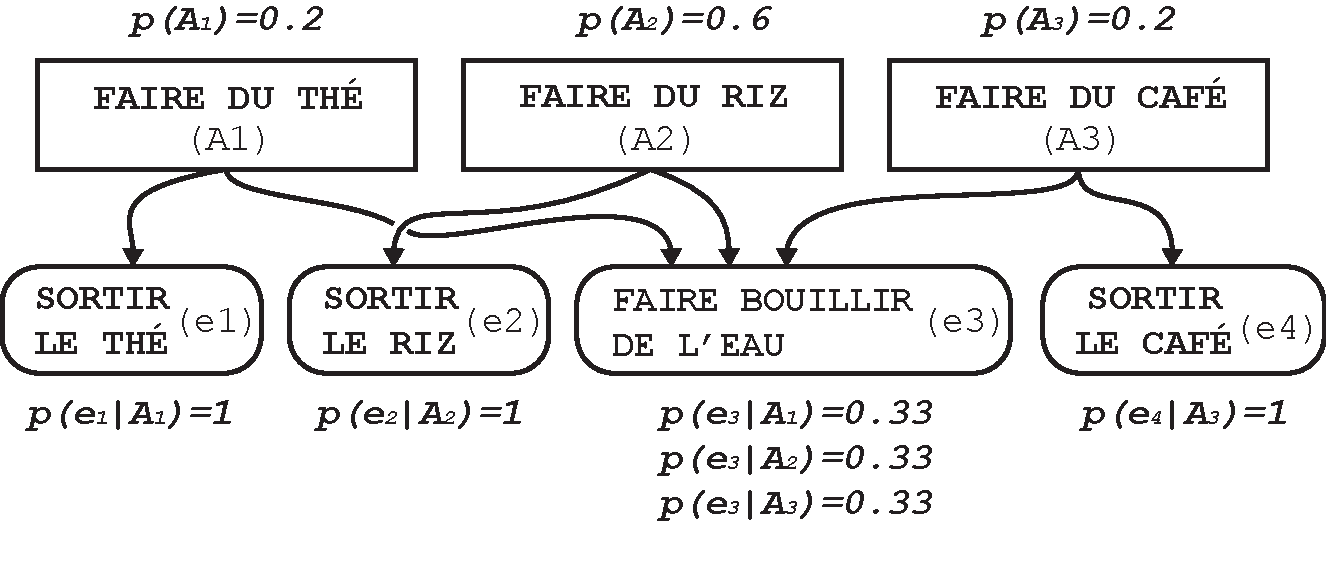
\includegraphics[width=0.8\linewidth]{learn_bayes.pdf}
	\caption{Schématisation d'un exemple de réseau bayésien naïf.}
	\label{fig:learn_bayes}
\end{figure}

\noindent Grâce aux données fournie par cet exemple, il est donc possible de réaliser l'application numérique suivante : 

\begin{align*}
	p(A_1|e_2)	& = \frac{p(e_2|A_1)\times p(A_1)}{p(e_2|A_1)\times p(A_1) + p(e_2|A_2)\times p(A_2) + p(e_2|A_3)\times p(A_3)} \\[10pt]
				& = \frac{0\times 0.2}{0\times 0.2 + 1\times 0.6 + 0\times 0.2} = 0 \\[20pt]
	p(A_2|e_2)	& = \frac{p(e_2|A_2)\times p(A_2)}{p(e_2|A_1)\times p(A_1) + p(e_2|A_2)\times p(A_2) + p(e_2|A_3)\times p(A_3)} \\[10pt]
				& = \frac{1\times 0.6}{0\times 0.2 + 1\times 0.6 + 0\times 0.2} = 1 \\[20pt]
	p(A_3|e_2)	& = \frac{p(e_2|A_3)\times p(A_3)}{p(e_2|A_1)\times p(A_1) + p(e_2|A_2)\times p(A_2) + p(e_2|A_3)\times p(A_3)} \\[10pt]
				& = \frac{0\times 0.2}{0\times 0.2 + 1\times 0.6 + 0\times 0.2} = 0
\end{align*}

\noindent Finalement, les probabilités sont mises à jour et il apparaît que l’activité \og \textit{faire du riz} \fg ($A_2$) est la seule activité possible puisque celle-ci admet une probabilité de $1$ lorsque l'évènement \og \textit{sortir le riz} \fg ($e_2$) est observé. Le système conclut donc que le résident de l'habitat intelligent est en train de préparer une portion de riz.

Les principaux avantages dans l'utilisation des réseaux bayésiens sont, la simplicité de leur implémentation ainsi que leur performance, tant en termes de taux de reconnaissance dans le cas des activités au sein d'un habitat intelligent, qu'en termes de temps d'exécution et de consommation d'espace mémoire \citep{Friedman1997}. Néanmoins, ceux-ci nécessitent de connaître l'ensemble des activités, des actions et des probabilités conditionnelles qui les relient pour fonctionner ; ce qui constitue un inconvénient majeur, car ces informations ne sont pas toujours disponibles.

Les modèles de Markov cachés (\aclp{HMM} ou \acsp{HMM}) ainsi que les champs aléatoires conditionnels (\aclp{CRF} ou \acsp{CRF}) sont d'autres exemples d'algorithmes statistiques qui ont été utilisés pour la reconnaissance d'activités au sein des habitats intelligents \citep{Oliver2004, Nazerfard2010, VanKasteren2011}. Les \acsp{HMM} peuvent être représentés comme des automates probabilistes à états finis dont l'évolution au cours du temps est entièrement déterminée par une probabilité initiale et des probabilités de transitions entre états. De plus, l'état du système, soit l'activité à reconnaître, n'est pas directement observable, mais caché par un processus d'observation. Autrement dit, au temps $t$, le système qui est dans l'état invisible $q_t$ émet l'observation $O_t$. Ces observations sont, quant à elles, visibles et elles peuvent, par exemple, correspondre à la valeur d'un capteur. Tout comme pour les réseaux bayésiens, les \acsp{HMM} offrent d’excellentes performances de reconnaissance et d’exécution. Néanmoins, la complexité de leur mise en place et de leur compréhension ainsi que la connaissance initiale requise pour leur fonctionnement sont autant de facteurs limitant leur utilisation à la reconnaissance d'un nombre très restreint d’activités. 

Par ailleurs, les \acsp{CRF} permettent, quant à eux, de modéliser les dépendances entre un ensemble d’observations réalisées sur une séquence et un ensemble d’étiquettes. En comparaison avec un \acs{HMM}, un \acs{CRF} ne repose pas sur l’hypothèse forte d’indépendance des observations entre elles, conditionnellement aux états associés (les activités). De plus, ils ne combinent pas de probabilités conditionnelles locales, évitant ainsi une estimation biaisée de ces probabilités si trop peu d’exemples étiquetés sont disponibles. Autrement dit, les \acsp{CRF} permettent de limiter le nombre de paramètres initiaux requis dans la mise en place d'un \acs{HMM}, offrant alors une généralisation du modèles de Markov.

\subsubsection{Les arbres de décision}

Les arbres de décision appartiennent à la catégorie des méthodes d'apprentissage supervisées. Comme illustré par la figure \ref{fig:learn_dtree}, la classification des données est faite par une suite de choix logiques représentée sous forme d'un arbre, où chacun de ses n\oe{}uds possède un unique parent excepté le n\oe{}ud racine. Ainsi, les feuilles de l'arbre correspondent aux classes des activités à reconnaître et les n\oe{}uds non terminaux sont des règles de classification qui doivent être vérifiées grâce aux attributs de la donnée qui est testée. 

\begin{figure}[H]
	\centering
	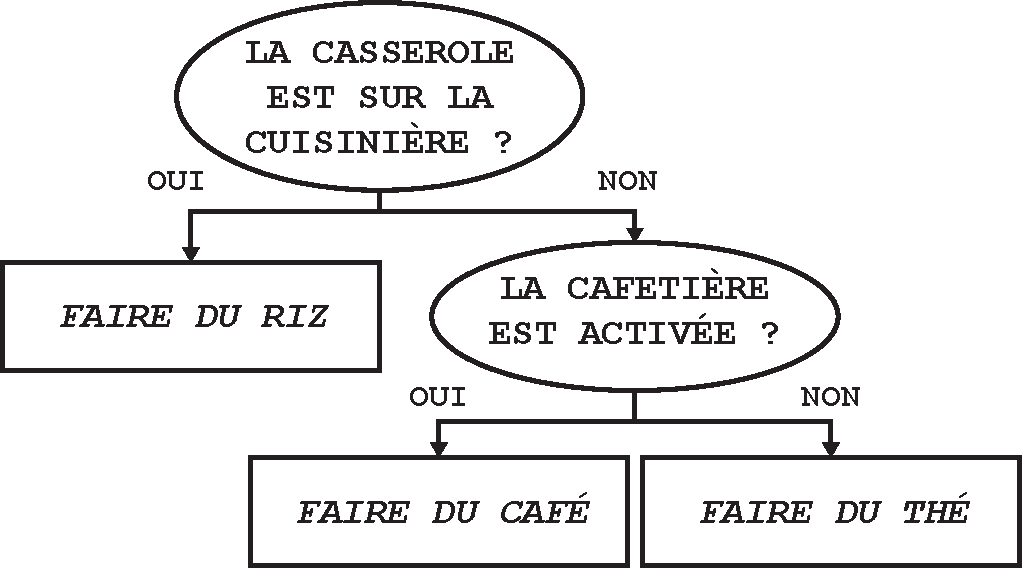
\includegraphics[width=0.7\linewidth]{learn_dtree.pdf}
	\caption{Schématisation d'un exemple d'arbre de décision binaire.}
	\label{fig:learn_dtree}
\end{figure}

Dans le domaine de la reconnaissance d'activités, les algorithmes d'arbres de décision qui sont les plus fréquemment utilisés sont, \ac{ID3} ainsi que son extension, C4.5 \citep{QuinlanRoss1993}. Les principales différences entre ces deux algorithmes sont qu'à l'inverse d'\acs{ID3}, C4.5 accepte les variables continues en plus des variables discrètes et ce dernier est également capable de gérer les données manquantes de façon automatique. Enfin, il permet de réduire le risque de sur-apprentissage, qui est très élevé avec l'algorithme \acs{ID3}, grâce à une technique de \textit{pruning} \citep{Bao2004, Ravi2005, Tapia2007}. Ce phénomène intervient lorsque le modèle d'apprentissage est trop similaire aux données d'entraînement et donc plus suffisamment générique pour reconnaître correctement de nouvelles activités. Malgré ces différences, le fonctionnement de ces deux algorithmes reste très similaire. Pour chaque attribut de l'ensemble de données qui n'a pas déjà été traité, son entropie $H$ (\textit{cf. } équation (\ref{eq:entropy})) est calculée. Ensuite, l'attribut ayant l'entropie la plus faible est sélectionné et une séparation des données est faite en fonction de celui-ci (\textit{p. ex.} \og \textit{la casserole est sur la cuisinière} \fg ou \og \textit{la casserole n'est pas sur la cuisinière} \fg). Enfin, la structure finale de l'arbre est créée de manière récursive en ne considérant uniquement les attributs qui n'ont jamais été sélectionnés, pour chaque sous-ensemble de données. Ceci vient donc conclure la phase d'entraînement d'un arbre de décision. La phase de reconnaissance, quant à elle, ne nécessite qu'un simple parcours de l'arbre. Ainsi, en reprenant l'exemple de la figure \ref{fig:learn_dtree}\textemdash si les données de l'instance à reconnaître correspondent au positionnement de la casserole sur la cuisinière de l'habitat intelligent, alors l'activité réalisée par le résident est \og \textit{faire du riz} \fg.

L'utilisation des arbres de décision offre plusieurs avantages. Dans un premier temps, ceux-ci restent relativement simples à implémenter, mais surtout, ils offrent une très grande facilité de compréhension. De plus, ils ont démontré une excellente performance tant en termes de rapidité d'exécution qu'en termes de taux de reconnaissance \citep{Bao2004}. En revanche, ils se sont révélés beaucoup moins efficaces dans des systèmes impliquant la reconnaissance d'un très grand nombre d'activités parmi lesquelles certaines peuvent se ressembler. De plus, les arbres de décision concèdent deux autres limites importantes qui sont, la nécessité d'avoir un très grand nombre de données pour être entraînés correctement et l'obligation de répéter la phase d'entraînement après chaque ajout d'une nouvelle activité ou après la modification des données d'une activité existante. 

\subsubsection{Le \textit{clustering}}

Les méthodes de \textit{clustering} représentent une large partie des algorithmes d'apprentissage non-supervisés \citep{Witten2011}. Le fonctionnement général de toutes les techniques de \textit{clustering} existantes consiste en la division homogène d'un ensemble de données en différents \textit{clusters} qui doivent partager des caractéristiques communes. Les \textit{clusters} sont donc des sous-ensembles des données d'apprentissage. La séparation des données en \textit{clusters} est réalisée, à la fois par minimisation de la distance intra-classe ; c'est-à-dire, la distance entre tous les éléments d'un même \textit{cluster}, ainsi que par la maximisation de la distance inter-classe, qui correspond à la distance entre tous les \textit{clusters}. Ensuite, pour chaque cluster, une donnée représentative lui est attribuée. En fonction de l'algorithme qui est employé, cette dernière peut être déterminée différemment. Dans certains cas, une nouvelle valeur (le barycentre) est calculée à l'aide des données déjà présentes dans le \textit{cluster}. Dans d'autres cas, c'est une donnée existante qui sera élue comme la plus représentative pour chaque \textit{cluster}. Un exemple d'une méthode de \textit{clustering} utilisant le calcul des barycentres est illustré en figure \ref{fig:learn_clustering}

L'algorithme de \textit{clustering} le plus utilisé dans le domaine de la reconnaissance d'activités est l'algorithme des $K$-moyennes \citep{Messing2009, Kovashka2010}. Cet algorithme requiert que le nombre total de \textit{clusters} $K$ soit fixé à l'avance. Ainsi, l'algorithme d'apprentissage commence par initialiser les barycentres, où la valeur qui leur est attribuée peut varier en fonction du problème à traiter. En effet, ceux-ci peuvent être initialisés à nul, avec des valeurs purement aléatoires ou encore avec des valeurs prises parmi les données existantes. Lorsque les barycentres sont définis, l'algorithme va, de manière itérative, commencer par calculer la distance de chaque instance de l'ensemble de données par rapport à chacun des $K$ barycentres. Chacune d'elles sera alors associée à son barycentre le plus proche. L'étape suivante consiste à mettre à jour la valeur des barycentres en fonction des \textit{clusters} qui se sont formés. Enfin, ce processus est répété jusqu'à l'obtention d'une convergence, c'est-à-dire, jusqu'à la stabilisation des valeurs des barycentres ; ce qui conduit à l'obtention du modèle d'apprentissage. Comme illustré dans l'exemple de la figure \ref{fig:learn_clustering}, ce modèle d'apprentissage admet trois \textit{clusters}, où chacun d'eux correspond au regroupement des données selon les trois mêmes activités qui sont utilisées depuis le début de ce chapitre. Dès lors, la classification d'une nouvelle instance nécessite de calculer la distance entre cette dernière et tous les barycentres. La plus petite distance obtenue détermine donc à quelle classe d'activité cette nouvelle donnée appartient. Dans cet exemple, la nouvelle donnée correspond donc à l'activité \og \textit{faire du café}\fg.

\begin{figure}[H]
	\centering
	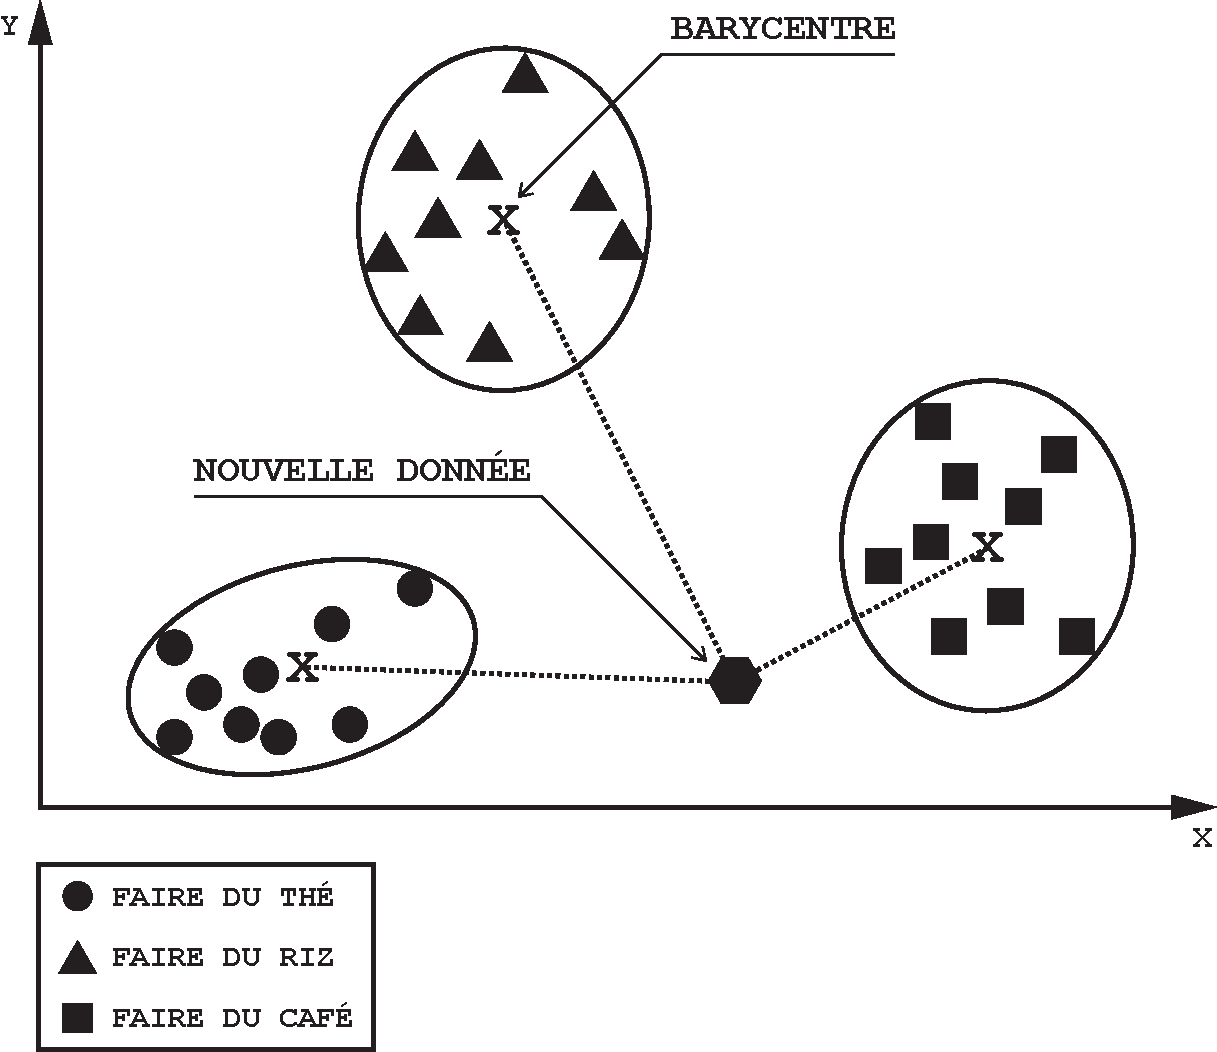
\includegraphics[width=0.6\linewidth]{learn_clustering.pdf}
	\caption{Schématisation d'un exemple d'algorithme de clustering.}
	\label{fig:learn_clustering}
\end{figure}

\noindent Parmi toutes les mesures de distance qu'il est possible d'utiliser, celle qui sont les plus fréquemment utilisé dans l'algorithme des $K$-moyennes lorsque les données ont $n$ dimensions sont, la distance Euclidienne $D_e$ et la distance de Manhattan $D_m$ respectivement rappelées par les équations (\ref{eq:dist_euclidean}) et (\ref{eq:dist_manhattan}) tel que,

\begin{equation}
	\label{eq:dist_euclidean}
	D_e = \sqrt{\sum_{i=1}^{n}(x_i-y_i)^2}
\end{equation}

\begin{equation}
	\label{eq:dist_manhattan}
	D_m = \sum_{i=1}^{n}\left|x_i-y_i\right|
\end{equation}

Bien que le côté non-supervisé de ces méthodes constitue un avantage majeur dans leur utilisation pour reconnaître des activités, elles n'en demeurent pas moins dénuées d'inconvénients. En effet, le processus d'entraînement est souvent coûteux en termes de temps d'exécution et en termes de consommation de la mémoire. De plus, le manque de flexibilité induit par la définition préalable du nombre de \textit{clusters} est un inconvénient majeur pour un système de reconnaissance où le nombre d'activités demeure potentiellement infini. Pour combler ce dernier inconvénient, il est possible de recourir à l'algorithme \ac{DBSCAN}, car son utilisation permet de s'affranchir d'une initialisation manuelle du nombre de clusters. Néanmoins, celui-ci éprouve des difficultés lorsqu'il s'agit de gérer des clusters ayant des densités différentes et ceci est fréquent dans le domaine de la reconnaissance d'activités. \acs{DBSCAN} n'est alors pas toujours le meilleur compromis.

\subsubsection{Les machines à support de vecteurs}

Les machines à support de vecteurs (\ac{SVM}) font partie des techniques d'apprentissage supervisées. L'objectif d'un \acs{SVM} est de créer une séparation des données d'entraînement optimale par le biais d'un hyperplan. De ce fait, l'algorithme va chercher à maximiser la marge, c'est-à-dire, la distance entre l'hyperplan et les données les plus proches de celui-ci. Ces données sont les supports de vecteurs. La figure \ref{fig:learn_svm_a} montre un exemple de machine à support de vecteurs linéaire. En revanche, il est possible que dans certains cas, les données ne soient pas linéairement séparables, c'est-à-dire qu'aucun hyperplan de marge optimale n'existe. Pour pallier cela, il est possible d'utiliser une fonction de noyau (linéaire, quadratique, polynomiale, de base radiale gaussienne, sigmoïde, \textit{etc.}). Celle-ci permet alors la conversion des données d'apprentissage en un ensemble de dimension supérieur, où il est possible de créer un hyperplan de marge optimale permettant de séparer les données, tel qu'illustré en figure \ref{fig:learn_svm_b}. Afin d'identifier à quelle classe d'activité la nouvelle donnée appartient, le processus de reconnaissance va simplement calculer de quel côté de l'hyperplan celle-ci se situe. Ainsi, dans le cas de l'exemple proposé en figure \ref{fig:learn_svm_a} la nouvelle donnée est à droite de l'hyperplan, elle est donc identifiée comme l'activité \og \textit{faire du café}\fg.

\begin{figure}[H]
	\centering
	\subfloat[Linéaire]{
		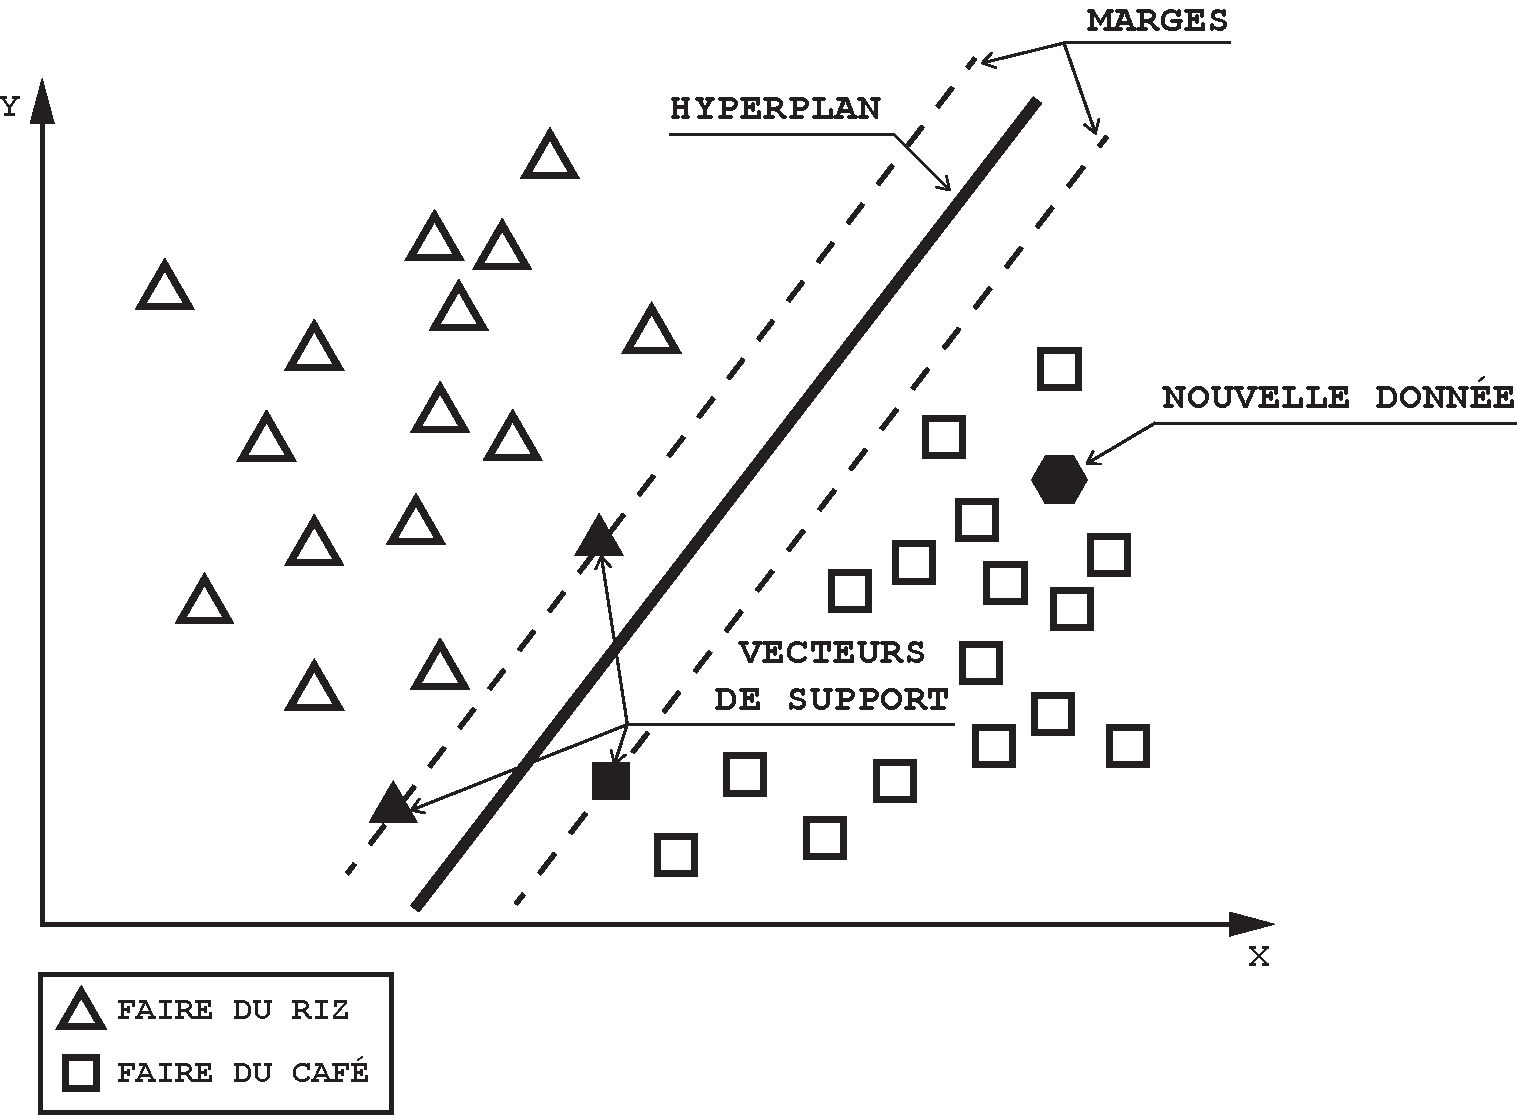
\includegraphics[width=.5\linewidth]{learn_svm_a.pdf}
		\label{fig:learn_svm_a}
	}
	\hspace*{\fill}
	\subfloat[Fonction de noyau]{
		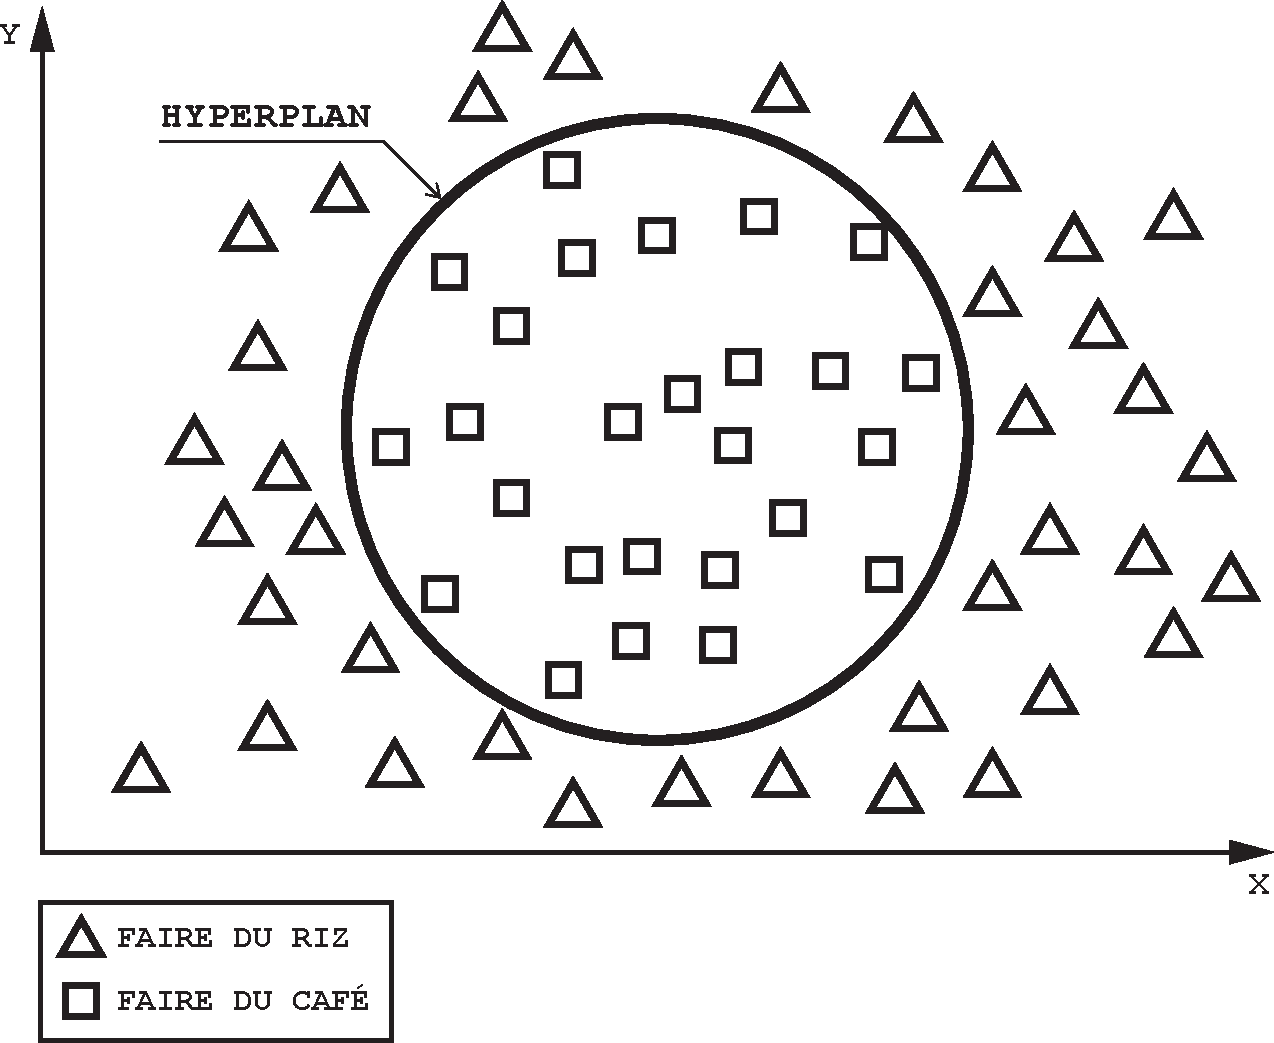
\includegraphics[width=.45\linewidth]{learn_svm_b.pdf}
		\label{fig:learn_svm_b}
	}
	\caption{Schématisation d'un SVM linéaire ainsi que d'un SVM utilisant une fonction de noyau.}
\end{figure}

Les \acs{SVM} sont souvent considérés comme des boîtes noires, car ils ne permettent pas l'extraction d'un modèle compréhensible, à l'inverse des arbres de décision par exemple. Néanmoins, ils sont fréquemment utilisés dans le domaine de la reconnaissance d'activités, pour plusieurs raisons \citep{He2009, Anguita2012}. La première est qu'ils permettent d'obtenir des taux de reconnaissance très élevés. De plus, le processus de reconnaissance est très efficace en termes de consommation des ressources et peut donc facilement être réalisé sur des systèmes portables. Toutefois, les machines à support de vecteurs ne sont pas adaptées pour traiter un très gros volume de données lors du processus d'apprentissage\textemdash ce dernier impliquant de lourds calculs pour construire le modèle.

\subsubsection{Les réseaux de neurones artificiels}

Les réseaux neurones artificiels (\aclp{ANN} ou \acsp{ANN}) sont des méthodes d’apprentissage qui peuvent être supervisées ou non-supervisées. Elles visent à imiter la pensée humaine par la modélisation simplifiée des systèmes neuronaux du cerveau de l’Homme et de l’animal. Les \acsp{ANN} sont composés de plusieurs neurones connectés entre eux qui s’échangent des signaux \citep{Witten2011}. Chaque neurone est composé d'un nombre $n$ d'entrées synaptiques qui sont chacune associées à un poids ($w$). Celles-ci sont ensuite agglomérées en une seule donnée grâce à un additionneur. Cette valeur est alors passée à une fonction d'activation qui va, pour chacun des neurones, renvoyer un signal de sortie positif ou négatif en fonction d'un certain seuil. Ainsi, pour effectuer un apprentissage supervisé avec les réseaux de neurones, la valeur des poids associés à chacune des synapses doit être modifiée afin que l’erreur entre les sorties du réseau et l'étiquette de la donnée testée soit atténuée. Dès que tous les poids sont mis à jour, la construction du modèle d'apprentissage est terminée et le processus reconnaissance peut commencer. La figure \ref{fig:learn_ann} montre un exemple simplifié d'un perceptron multicouche, l'une des implémentations possibles des \acsp{ANN}, permettant de reconnaître deux activités, \og \textit{faire du riz} \fg et \og \textit{faire du café} \fg. Dans cet exemple, les neurones d'entrée admettent les valeurs des capteurs de l'environnement intelligent et les neurones de sorties correspondent aux activités à reconnaître. Pour simplifier l'exemple, les valeurs de sorties sont exprimées sous la forme de booléens, mais les \acsp{ANN} expriment normalement les sorties sous la forme de probabilités. Par conséquent, c'est la probabilité la plus élevée qui détermine l'étiquette de la donnée testée. Dans ce cas, lorsque le placard est ouvert ; que de l'eau s'écoule du robinet ; que la plaque de cuisson avant-gauche est allumée ; que la casserole est sur la cuisinière et que la cafetière n'est pas allumée, l'activité prédite par cet \acs{ANN} est \og \textit{faire du riz} \fg.

\begin{figure}[H]
	\centering
	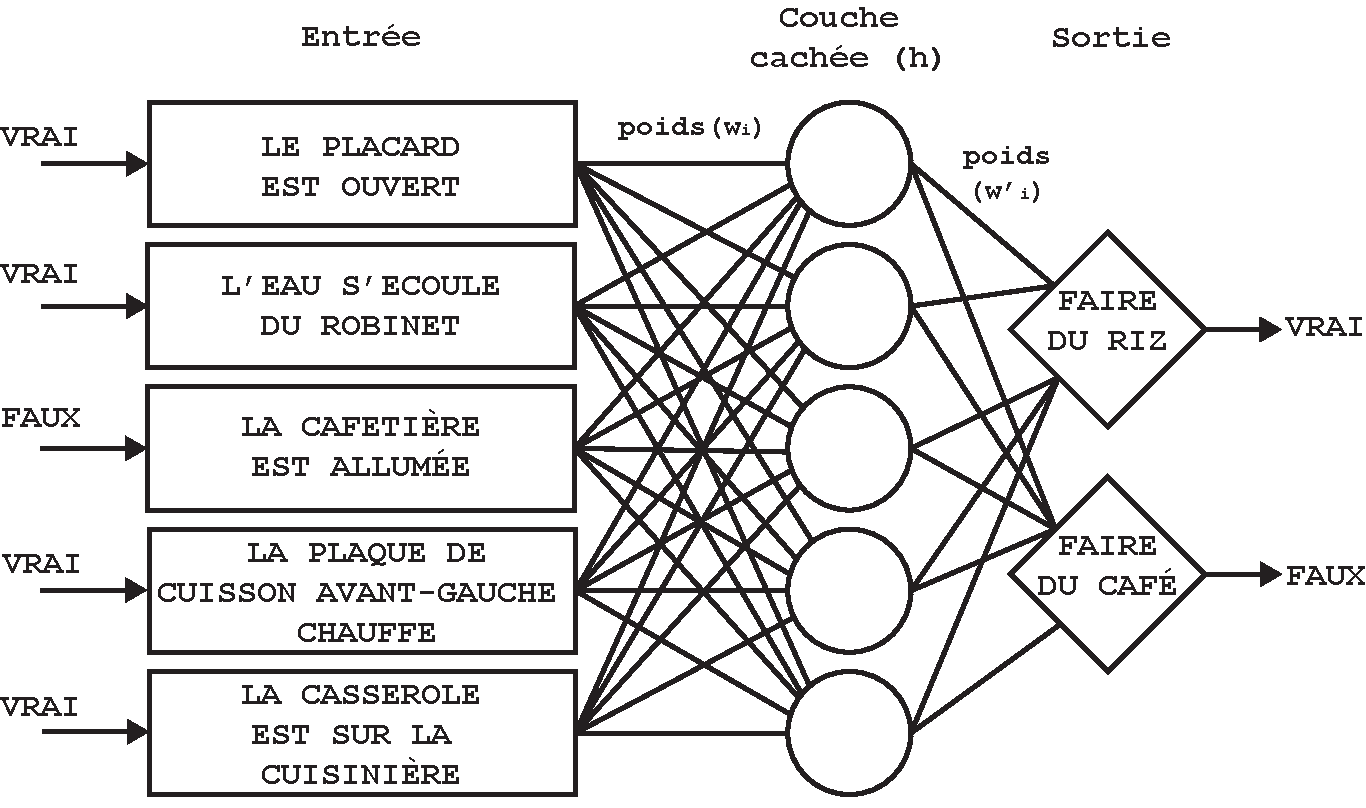
\includegraphics[width=0.8\linewidth]{learn_ann.pdf}
	\caption{Schématisation d'un exemple de réseau de neurones artificiels.}
	\label{fig:learn_ann}
\end{figure}

De nombreux travaux dans le domaine de la reconnaissance d'activités ont démontré la performance des \acsp{ANN} ainsi que leur robustesse quant à l'exploitation de données fortement bruitées \citep{Parkka2006, Delachaux2013}. Néanmoins, ces techniques nécessitent un temps d'apprentissage considérable pouvant atteindre plusieurs jours. Ceci demeure un inconvénient majeur d'autant plus que ce processus doit être reproduit après chaque ajout d'une nouvelle activité ou après la modification d'une activité déjà existante. De plus, il est très facile, pour un système de reconnaissance basé sur un réseau neural, de tomber dans le sur-apprentissage.

Dans la dernière décennie, l'augmentation exponentielle de la puissance des appareils informatiques a permis de propulser l'utilisation des techniques d'apprentissage profond (deep learning) qui sont des applications particulières des \acsp{ANN} traditionnels. Celles-ci ont démontré leur excellente performance de reconnaissance dans beaucoup de domaines, dont celui de la reconnaissance d'activités \citep{Yang2015, Li2016, Wang2018}. Bien qu'il soit possible que les techniques d'apprentissage profond soient capables de traiter des données brutes directement, c'est-à-dire de se passer de toutes les étapes préliminaires pour la construction du modèle d'apprentissage, elles admettent encore de nombreux inconvénients additionnels à ceux des \acsp{ANN}. En effet, les modèles sont souvent utilisés comme des boîtes noires, car lorsque les résultats obtenus ne sont pas satisfaisants, il est pratiquement impossible d'en expliquer les raisons et surtout de trouver des solutions pour remédier au problème. De plus, ces techniques requièrent un volume conséquent de données pour être entraînées correctement et ainsi, obtenir un modèle générique et réutilisable.

\subsection{La mesure de la performance}

L'étape finale du processus d'apprentissage pour la reconnaissance d'activités consiste en une évaluation de la performance du système. Pour ce faire, il existe de nombreuses métriques qui s'appuient sur l'utilisation d'une matrice de confusion \citep{Fawcett2006}. Cette dernière permet l'identification de la relation qui lie la classe actuelle d'un enregistrement et celle qui est prédite par l'algorithme d'apprentissage. Par exemple, la matrice de confusion retournée par l'un de ces algorithmes dans le cas d'une reconnaissance binaire est donnée par le tableau \ref{tab:conf_mat}. Lorsqu'une instance est positive et qu'elle est prédite comme positive, alors il s'agit d'un vrai positif ($VP$), sinon c'est un faux négatif ($FN$). Dans le cas contraire, si l'instance est négative, et qu'elle est prédite comme positive, alors s'agit d'un vrai négatif ($VN$), sinon c'est un faux positif ($FP$).

\begin{table}[H]
	\begin{center}
		\caption{Matrice de confusion d'un système de reconnaissance binaire.}
		\label{tab:conf_mat}
		\begin{tabular}{llllllllll}
			\cline{3-4}
			& \multicolumn{1}{l|}{} & \multicolumn{2}{c|}{\textbf{classe prédite}} \\ \cline{3-4}
	        & \multicolumn{1}{l|}{} & \multicolumn{1}{c|}{\textbf{oui}} & \multicolumn{1}{c|}{\textbf{non}} \\ \cline{1-4}
			\multicolumn{1}{|c|}{\multirow{2}{*}{\textbf{classe actuelle}}} & \multicolumn{1}{c|}{\textbf{oui}} & \multicolumn{1}{c|}{$VP$} & \multicolumn{1}{c|}{$FN$} \\ \cline{2-4}
			\multicolumn{1}{|c|}{} & \multicolumn{1}{c|}{\textbf{non}} & \multicolumn{1}{c|}{$FP$} & \multicolumn{1}{c|}{$VN$} \\ \cline{1-4}
		\end{tabular}
	\end{center}
\end{table}

Parmi l'ensemble des métriques permettant d'évaluer la performance d'un algorithme d'apprentissage, la mesure de la justesse est la plus fréquemment utilisée, du fait de sa simplicité. Elle permet de déterminer le ratio entre le nombre de prédictions correctement réalisées et le nombre total de cas tel que, 
\begin{equation}
	justesse = \frac{VP+VN}{VP+FP+VN+FN} 
\end{equation}

Néanmoins, malgré sa popularité, la justesse ne permet pas d'évaluer avec robustesse la qualité des prédictions. En effet, cette dernière ne prend pas en considération les prédictions qui peuvent être faites par chance. Par conséquent, une bonne justesse n'implique pas nécessairement une bonne performance de reconnaissance. C'est le phénomène du \textit{paradoxe de la justesse}. Pour tenir compte de cet effet de bord souvent négligé, d'autres métriques comme la Kappa de Cohen $k$ ou la F-mesure doivent être calculées \citep{Ben-David2007a}. La première est exprimée par : 

\begin{equation}
	\label{eq:kappa}
	k = \frac{P_o - P_e}{1 - P_e}
\end{equation}

\noindent où $P_o$ et $P_e$ sont respectivement, les probabilités observées, c'est-à-dire le taux de succès obtenu par l'algorithme ; et les probabilités espérées, c'est-à-dire le taux de succès hypothétique de l'algorithme. La relation (\ref{eq:f-score}) permet, quant à elle, d'obtenir la F-mesure, tel que,

\begin{equation}
	\label{eq:f-score}
	F\mbox{-} Score = 2 \cdot \frac{pr\acute{e}cision \cdot rappel}{pr\acute{e}cision + rappel}
\end{equation}

\noindent où la $pr\acute{e}cision$ et le $rappel$ sont respectivement donnés par les équations (\ref{eq:precision}) et (\ref{eq:rappel}) tel que, 

\begin{equation}
	\label{eq:precision}
	Pr\acute{e}cision = \frac{VP}{VP+FP}
\end{equation}

\begin{equation}
	\label{eq:rappel}
	Rappel = \frac{VP}{VP+FN}
\end{equation}

\section{Conclusion}

Dans un premier temps, ce chapitre s'est intéressé aux habitats intelligents existants qui ont été regroupés en trois catégories. Premièrement, les habitats intelligents académiques \acs{LIARA} et le laboratoire \acs{DOMUS} sont deux architectures qui reposent sur des technologies héritées du milieu industriel. Ces deux habitats, dont le coût total est très dispendieux, ont démontré une faiblesse en termes d'évolutivité et, par conséquent, l'absence d'une quelconque solution pour y intégrer facilement des \textit{wearable devices}. Ensuite, les architectures d'habitats basés composants comme Gator-Tech ou Amiqual4home ont répondu à cette problématique, car elles ce sont révélés beaucoup plus flexibles quant à l'intégration de nouveaux composants matériels qu'ils soient de type ambiant ou portable. Néanmoins, la surcharge du serveur central pouvant être occasionnée par un grand nombre de flux de données n'en fait pas pour autant la solution idéale. Enfin, les architectures basées sur un réseau maillé, plus récentes, sont apparues comme les plus avancées en terme de flexibilité pour y intégrer des \textit{wearable devices} malgré le support de la technologie de communication ZigBee uniquement. 

Dans sa deuxième partie, ce chapitre a présenté plus en détail l’ensemble des étapes nécessaires pour réaliser le processus d'apprentissage pour reconnaître des activités. Les différentes techniques permettant de raffiner la qualité des données brutes renvoyées par les différemment capteurs et qui constituent la première phase du processus ont été exposés. Ensuite, les algorithmes de d'apprentissage les plus utilisés dans le domaine de la reconnaissance d'activités ont été examinés. Finalement, ce chapitre s'est achevé par la description des différentes méthodes permettant d'évaluer la performance de ces algorithmes et de la qualité intrinsèque de la reconnaissance d'activités.
\let\cleardoublepage\clearpage
\chapter{les wearable devices au sein des habitats intelligents}
\label{chap:3}

Dans le chapitre précédent, le processus d'apprentissage pour la reconnaissance d'activités a été présenté dans un cas d'application générique. De nombreuses étapes, depuis l'obtention des données brutes jusqu'à la classification des activités à reconnaître, y ont été détaillées. Néanmoins, dans un contexte d'utilisation avec des \textit{wearable devices}, la manière dont ces données sont acquises n'a, quant à elle, pas été mentionnée. De plus, l'adaptation de ce processus avec ces dispositifs fait intervenir une étape supplémentaire de transmission des données. Ce chapitre va donc commencer par donner une définition de ce que sont les \textit{wearable devices}, puis il traitera plus en détail des composants matériels et logiciels qui sont plus spécifiques dans l'utilisation de ces dispositifs au sein des habitats intelligents.

\section{Définitions}

Selon le rapport publié par l'\cite{InternationalTelecommunicationUnion2012}, l'internet des objets (\acl{IoT} ou \acs{IoT}) représente une \og infrastructure mondiale pour la société de l'information, qui permet de disposer de services évolués en interconnectant des objets (physiques ou virtuels) grâce aux technologies de l'information et de la communication interopérables existantes ou en évolution \fg. Ainsi, D'un point de vue conceptuel, l'\acs{IoT} caractérise des objets physiques connectés ayant leur propre identité numérique et capables de communiquer les uns avec les autres. Ce réseau crée en quelque sorte une passerelle entre le monde physique et le monde virtuel. D'un point de vue technique, l'\acs{IoT} consiste en l'identification numérique directe et normalisée (adresse IP, protocoles de communication, \textit{etc.}) d'un objet physique grâce à un système de communication sans-fil qui peut être du Bluetooth ou encore du Wi-Fi. 

Par conséquent, les \textit{wearable devices} appartiennent aux objets connectés, puisqu'ils se caractérisent plus particulièrement comme une technologie qui embarque des capteurs et qui est disposée directement sur le corps humain. \cite{Godfrey2018} ont identifié deux types de \textit{wearable devices} : les dispositifs autonomes (\textit{p. ex.} les moniteurs d'activités physiques) et les dispositifs de mesure (\textit{p. ex.} un moniteur de fréquence cardiaque porté sur la poitrine). Les dispositifs autonomes permettent de réaliser différents traitements, plus ou moins complexes, dont les résultats sont ensuite communiqués à d'autres appareils, tandis que les dispositifs de mesure ont, quant à eux, pour seul objectif de transférer les informations du capteur. 

Les principaux avantages offerts par les \textit{wearable devices}, comme leur taille, leur faible prix ou leur facilité d'utilisation, ont favorisé leur usage dans différents domaines de recherche tels que la surveillance des activités physiques et sportives, la surveillance en continu de la santé ou encore la reconnaissance de gestes, d'activités ou de chutes. \citep{Seon-WooLee2002, Istepanian2011, Garcia-Ceja2014, Bayat2014a, YuanJieFan2014, Gao2014a, Nielsen2014b, Adib2015, Davis2016, Khan2016, Chapron2018}.

\section{Les capteurs}

Pour réaliser le processus d'apprentissage permettant de mettre en place une reconnaissance, la première étape consiste à récolter des données brutes qui sont produites par des capteurs. Cependant, puisqu'il en existe une grande diversité, il semble nécessaire d'identifier ceux qui sont les plus adéquats pour être proposés en tant que \textit{wearable devices}. Pour ce faire, cette section va présenter, en ce basant sur la taxonomie d'\cite{Acampora2013}, les capteurs parmi ceux qui sont les plus utilisés dans ce domaine d'application.

\subsection{Les capteurs de mouvements}

Les centrales inertielles (\aclp{IMU} ou \acsp{IMU}) sont les capteurs de mouvement qui sont le plus fréquemment implantés dans les \textit{wearable devices} de part leur simplicité d'utilisation. Celles-ci peuvent comporter d'un à trois types de capteurs différents : les accéléromètres, les gyroscopes et les magnétomètres. Ils permettent de mesurer respectivement l'accélération linéaire, la vitesse angulaire et l'intensité du champ magnétique que subissent les objets auxquels ils sont fixés, grâce à un maximum de trois axes orthogonaux ($x,\: y\: $ et $\: z$). L'adoption de ces capteurs a permis de nombreuses applications concrètes, telles que la reconnaissance de chutes chez les personnes âgées, l'identification de l'orientation du corps, la réadaptation, ainsi que la reconnaissance d'activités quotidiennes \citep{Seon-WooLee2002, Garcia-Ceja2014, Bayat2014a, Gao2014a, Davis2016, Chapron2018}.

\subsection{Les capteurs physiologiques}

Grâce au progrès technologique et plus particulièrement à la miniaturisation de l'électronique, de nouveaux types de capteurs, jusqu'alors réservés au domaine médical, ont pu être utilisés pour récolter les données physiologiques des utilisateurs, sans pour autant recourir aux services spécialisés d'un hôpital. Cependant, certaines techniques sont encore considérées comme complexes et intrusives à la fois. C'est, par exemple, le cas de l'\ac{EEG} qui demeure encore rarement exploité. Ce capteur physiologique permet la d'obtenir la représentation l'activité électrique du cerveau par l'intermédiaire d'électrodes disposées sur le crâne d'un individu. Néanmoins, plusieurs autres capteurs physiologiques ont, quant à eux, été très largement utilisés, et ce, dans de nombreux domaines de recherche. Parmi ceux-ci, il est possible de mentionner les capteurs qui permettent l'acquisition de l'\ac{ECG}, c'est-à-dire, la représentation graphique de l'activité électrique du c\oe{}ur ; de l'\ac{EMG}, soit l'activité électrique produite par les muscles ; de capteurs mesurant la glycémie, qui indique le taux de concentration de glucose dans le sang, ou de la \ac{SPO2}, qui désigne le taux de saturation du sang en oxygène. Au sein des habitats intelligents, l'intégration de ces capteurs dans des \textit{wearable devices} a principalement permis de proposer de nouvelles techniques pour la réhabilitation \citep{YuanJieFan2014}, la reconnaissance de gestes \citep{Jung2015, Benatti2015, Tavakoli2018} et la surveillance en continu de la santé des résidents pour détecter de possibles maladies \citep{Istepanian2011, Adib2015, Khan2016}.

\subsection{Les capteurs de courbure et de force}

Certains dispositifs considérés comme des \textit{wearable devices} tels que les gants présentés par \cite{Sanford2015} et \cite{Zheng2016} ainsi que les chaussures conçues par \cite{Bamberg2008} et \cite{Bae2013}, ont nécessité l'utilisation de capteurs de courbure (\textit{flex sensors}) et de force (\aclp{FSR} ou \acsp{FSR}). Ces capteurs fonctionnent grâce à des résistances dont la valeur change respectivement en fonction de la courbe qui est donnée au capteur ou de la pression qui est appliquée sur la surface de contact. Ainsi, comme illustré par ces différentes recherches, ces capteurs se sont montrés utiles dans certaines applications de réadaptation et de reconnaissance de gestes et d'activités. La figure \ref{fig:flex_force_sensors} montre respectivement un capteur de courbure (\ref{fig:flex_sensor}) ainsi qu'un capteur de force (\ref{fig:force_sensor}).

\begin{figure}[H]
    \centering
	\subfloat[Capteur de courbure]{
		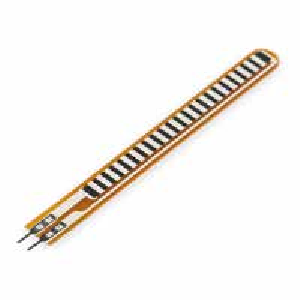
\includegraphics[width=.35\linewidth]{flex_sensor.pdf}
		\label{fig:flex_sensor}
    }
    \hspace*{2cm}
	\subfloat[Capteur de force (\acs{FSR})]{
		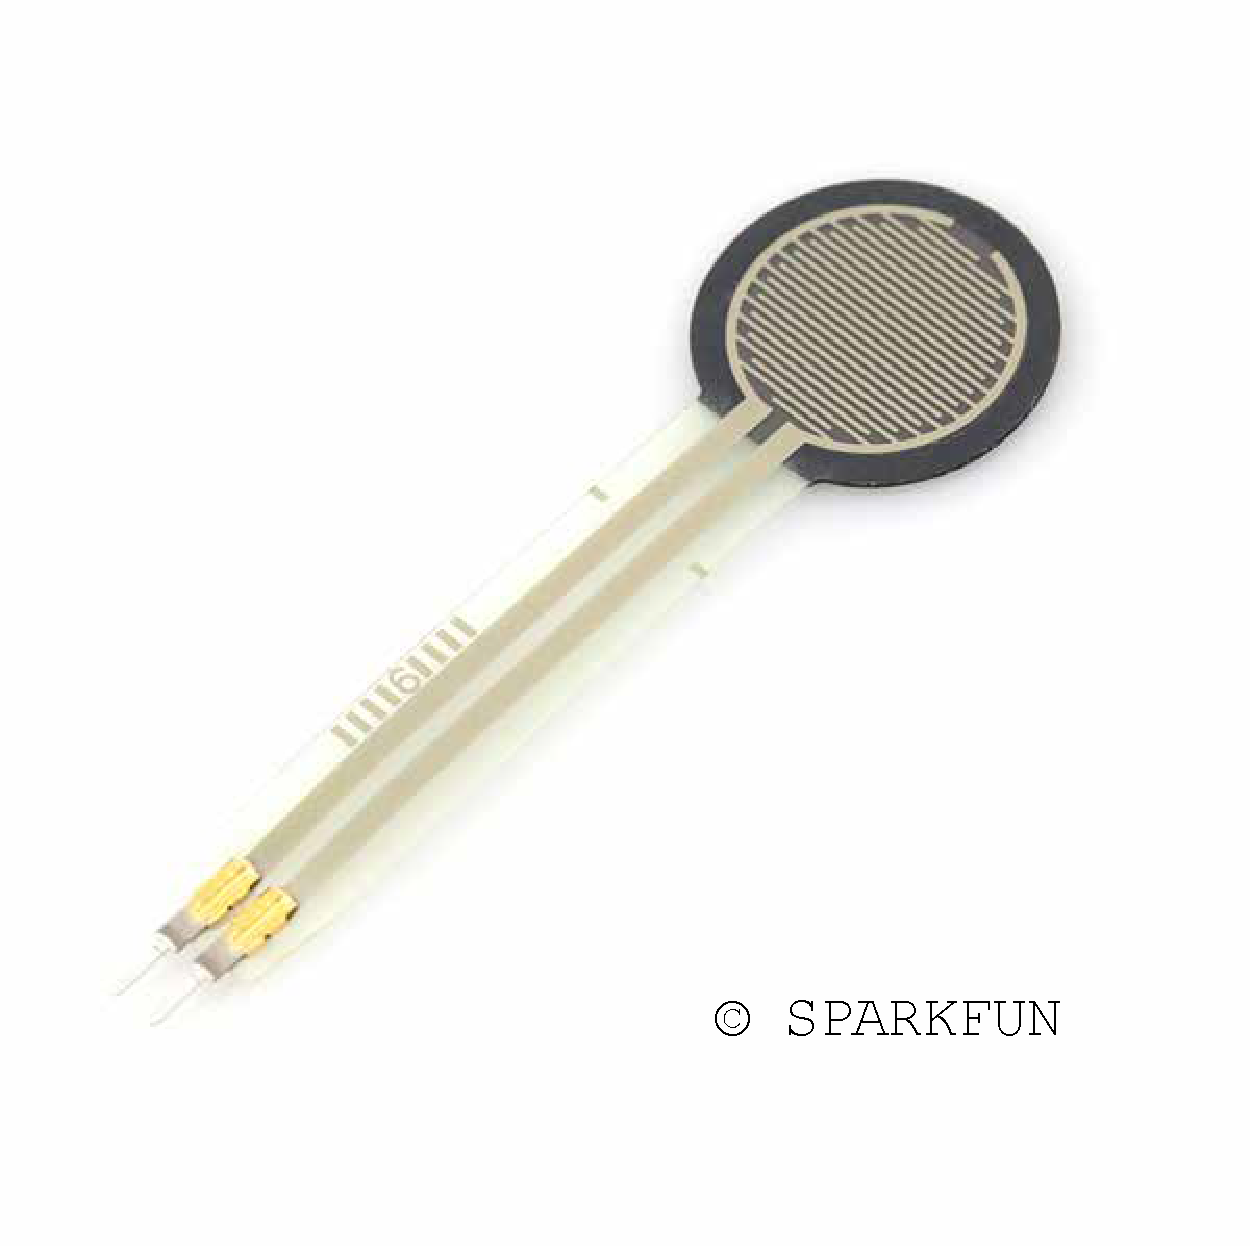
\includegraphics[width=.35\linewidth]{force_sensor.pdf}
		\label{fig:force_sensor}
    }
    \caption{Exemples de capteurs de courbure et de force, respectivement situés à gauche et à droite.}
    \label{fig:flex_force_sensors}
\end{figure}

\subsection{Les capteurs de environnementaux}

Les capteurs environnementaux comportent principalement les capteurs de pression barométrique, d'humidité, de température et de dioxyde de carbone (CO\textsubscript2). Ils sont principalement utilisés pour fournir des informations relatives à l'environnement proche des utilisateurs de \textit{wearable devices}. Ainsi, les données produites par ce type de capteur peuvent être utilisées pour identifier le contexte d'utilisation dans lequel leurs porteurs évoluent et par conséquent, renforcer les analyses réalisées grâce aux autres capteurs \citep{Acampora2013}. Par ailleurs, certains capteurs d'humidité et de température ont également été utilisés pour fournir des informations nécessaires à la surveillance de l'état de santé des utilisateurs des \textit{wearable devices} \citep{Anliker2004}.

\section{Les technologies de communication sans-fil}

Lorsqu'il est appliqué à des \textit{wearable devices}, le processus d'apprentissage nécessite une étape supplémentaire qui est la transmission de données. Ces dernières peuvent être les données brutes, les caractéristiques ou les décisions qui sont émises en sortie de l'algorithme d'apprentissage. En fonction des cas et des capteurs que peut comporter le dispositif, la fréquence d'émission ainsi que le poids des données à transmettre peut fortement varier. Ainsi, il est nécessaire de choisir une technologie de communication sans-fil adéquate pour chaque situation. Cette section va donc s'intéresser à celles qui sont les plus communément utilisées par les \textit{wearable devices} existants.

\subsection{Les topologies des réseaux}
\label{sec:topo}

Avant d'entrer dans le détail des technologies de communication utilisées par les \textit{wearable devices}, il est important de commencer par énoncer les topologies de réseaux existantes dans le domaine du sans-fil. En effet, elles jouent un rôle important dans le bon fonctionnement de la communication réseau et l'identification de de leur différentes caractéristiques va permettre, \textit{a posteriori}, de mieux cibler les besoins pour le développement de nouveaux systèmes. D'après \cite{Tanenbaum2011}, les topologies les plus fréquemment mises en place dans un contexte sans-fil sont :

\begin{itemize}[label=\textbullet]
	\item
	      La \textbf{diffusion (\textit{broadcast})} (figure \ref{fig:topo_broadcast}) où un message est envoyé par un n\oe{}ud émetteur à tous les n\oe{}uds récepteurs du réseau qui sont à sa portée. Le canal de communication est unidirectionnel et aucun accusé de réception n'est transmis au n\oe{}ud émetteur depuis les n\oe{}uds récepteurs.
	\item
          Les \textbf{réseaux en étoile} (figure \ref{fig:topo_star}) admettent un n\oe{}ud émetteur-récepteur central qui communique, à travers plusieurs canaux bidirectionnels, avec plusieurs autres n\oe{}uds émetteurs-récepteurs périphériques. Ces émetteurs-récepteurs périphériques ne peuvent pas communiquer directement les uns avec les autres. 
    \item 
        Les \textbf{réseaux pair-à-pair (\acl{P2P} ou \acs{P2P})} permettent à deux n\oe{}uds émet\-teurs-récepteurs, reliés par un canal de communication bidirectionnel, d'échanger des données dans les deux sens, tel qu'illustré par la figure \ref{fig:topo_p2p}.
    \item
        Les \textbf{réseaux maillés} (figure \ref{fig:topo_mesh}) permettent l'échange de données entre n'importe quels n\oe{}uds du réseau sans passer par un n\oe{}ud central. La communication est bidirectionnelle et chaque n\oe{}ud peut-être relié à plusieurs autres n\oe{}ud qui composent le réseau.
    \item
        Le \textbf{mode scan} (figure \ref{fig:topo_scan}) permet à un n\oe{}ud central de fonctionner en mode réception, c'est-à-dire, en attente de recevoir un signal provenant de n'importe quel n\oe{}ud émetteur qui est à sa portée. La communication entre les deux n\oe{}uds est unidirectionnelle et se fait du n\oe{}ud émetteur vers le n\oe{}ud central.
\end{itemize}

\begin{figure}[H]
    \centering
    \subfloat[Diffusion]{
        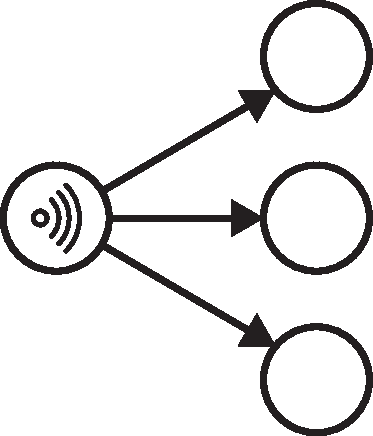
\includegraphics[width=.2\linewidth]{topo_broadcast.pdf}
        \label{fig:topo_broadcast}
    } 
    \hspace*{.2\linewidth}
    \subfloat[Étoile]{
        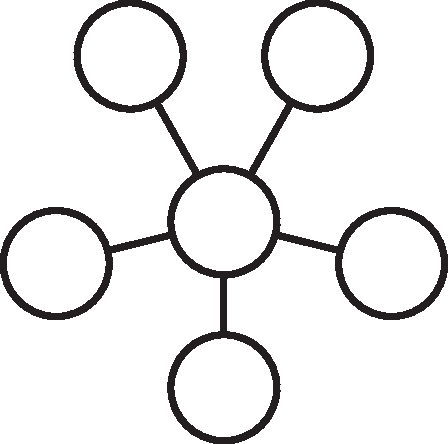
\includegraphics[width=.22\linewidth]{topo_star.pdf}
        \label{fig:topo_star}
    }
    \\[30pt]
    \subfloat[Pair-à-Pair]{
		
\includegraphics[width=.3\linewidth]{topo_p2p.pdf}
		\label{fig:topo_p2p}
    }
    \hspace*{.1\linewidth}
	\subfloat[Maillé]{
		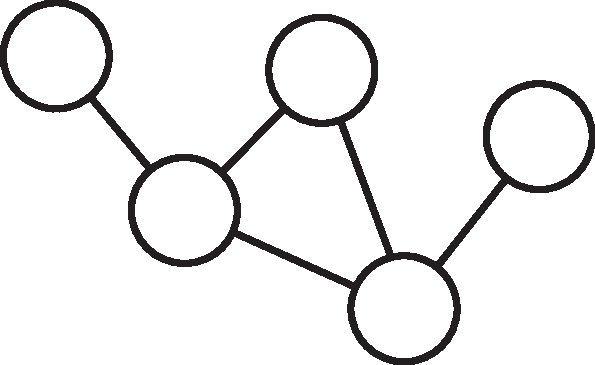
\includegraphics[width=.3\linewidth]{topo_mesh.pdf}
		\label{fig:topo_mesh}
    }
    \\[30pt]
    \subfloat[Mode scan]{
		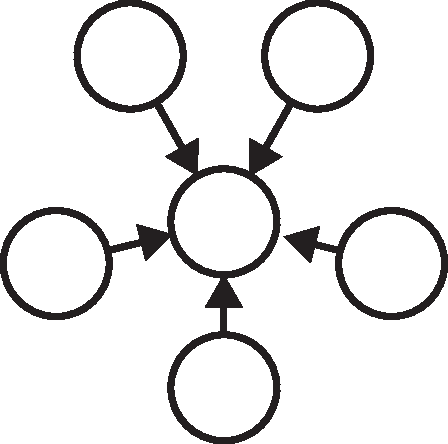
\includegraphics[width=.22\linewidth]{topo_scan.pdf}
		\label{fig:topo_scan}
    }
	\caption{Représentation des topologies réseaux pour les technologies de communication sans-fil.}
\end{figure}

\subsection{Wi-Fi}
Le Wi-Fi, régi par le standard IEEE 802.11\footnote{\url{https://goo.gl/X9WKyx}}, est probablement la technologie de communication sans-fil la plus connue, car nous l'utilisons massivement depuis deux décennies. En constante amélioration, chaque génération du standard a apporté aussi bien des vitesses plus rapides et une latence réduite, qu'une meilleure expérience utilisateur dans une multitude d’environnements et avec divers types de périphériques. Le standard qui est actuellement le plus utilisé est le Wi-Fi 802.11ac. Bien qu'il offre des vitesses de transfert de données à haut débit (de 400 Mbit/s à 6 Gbit/s), sa portée reste dans la moyenne de celles proposées par d'autres technologies, soit une centaine de mètres. Par ailleurs, le plus gros inconvénient du Wi-Fi 802.11ac demeure sa forte consommation énergétique, ce qui est un facteur extrêmement limitant pour les objets connectés (\acs{IoT}), parmi lesquels se retrouvent les \textit{wearable devices}. 

Dans un futur proche, les évolutions prévues dans les standards 802.11ah et 802.11ax vont principalement se concentrer sur l'amélioration de la consommation énergétique afin que l'utilisation du Wi-Fi devienne adaptée pour l'\acs{IoT}. Néanmoins, la contrepartie de cette évolution est l'impact sur la vitesse de transfert de données, qui va alors, devenir beaucoup plus faible (8 Mbit/s) \citep{Sun2013}. 

\subsection{Bluetooth Low Energy (\acs{BLE})}
\label{subec:com_ble}

Le \acs{BLE}\footnote{\url{https://www.bluetooth.com/specifications}} a été lancé en 2010 dans le cadre de la spécification du Bluetooth 4.0. Bien souvent, il est considéré comme une version plus légère et plus optimisée du Bluetooth classique (versions 1 à 3), mais en réalité, le \acs{BLE} présente une conception totalement différente. En effet, ce dernier a été pensé pour être une technologie de communication proposant une consommation d'énergie très faible, spécifiquement optimisée pour pouvoir offrir un coût réduit, une faible bande passante, ainsi qu'une complexité moindre. En comparaison aux autres technologies de communication sans-fil à faible consommation, le \acs{BLE} a connu une adoption très rapide principalement grâce à la croissance phénoménale des téléphones intelligents et plus généralement de l'informatique mobile. Ainsi, les leaders de l’industrie mobile comme Apple ou Samsung ont favorisé le large déploiement de cette technologie qui est aujourd'hui, la technologie de communication la plus utilisée par les \textit{wearable devices} \citep{Gomez2012b}. 

D'autre part, avec l'arrivée des premiers appareils supportant la version 5 du Bluetooth, cette technologie devient la seule à supporter l'intégralité des topologies réseaux présentées dans la section \ref{sec:topo}. En effet, en plus d'offrir un débit et une portée deux fois supérieurs à celui de la quatrième version, soit 2 Mbit/s et 250 mètres respectivement, cette nouvelle spécification intègre également la nouvelle norme : \og Bluetooth Mesh 1.0 \fg, qui va permettre la mise en place d'un réseau maillé\footnote{\url{https://www.bluetooth.com/specifications/mesh-specifications}}. Cependant, il ne sera pas possible de tirer profit de tous ces nouveaux avantages en même temps, puisque cette cinquième version permettra deux modes de fonctionnement : haut débit ou longue portée. Ainsi, dans le premier cas, la vitesse de transfert sera favorisée au profit de la portée et inversement, ceci dans le but de continuer les efforts pour la réduction de la consommation d'énergie tout en améliorant les capacités.

\subsection{ZigBee}

La technologie ZigBee a été développée dans les années 1990 et avec l'avènement des objets connectés, elle est devenue l'une des technologies de communication parmi les plus utilisées. En comparaison avec le Wi-Fi, le ZigBee admet l'avantage de ne consommer que peu d'énergie. De plus, le standard IEEE 802.15.4\footnote{\url{https://goo.gl/X9WKyx}}, qui régit cette technologie, précise que le ZigBee admet une portée comprise entre 10 et 100 mètres, en fonction de la puissance de l'émetteur et de certaines caractéristiques environnementales, soit autant que la plupart des autres technologies de communication présentées dans ce chapitre. 

Initialement, le ZigBee a été introduit pour répondre à des problématiques liées à l'hétérogénéité de l'\acs{IoT} \citep{Rahmani2015, Cho2013} et par extension, des technologies présentes au sein des habitats intelligents \citep{Hui2017}. En effet, dès le début, le ZigBee a offert la possibilité de s'appuyer sur la conception d'une topologie de réseau maillé (\textit{mesh}), ce qu'aucune autre technologie de communication présentée précédemment ne permettait avant l'apparition d'une norme identique dans la nouvelle version du \acs{BLE}. De ce fait, certains \textit{wearable devices} \citep{Cruz2018} et habitats intelligents \citep{Cook2013} ont vite adopté cette technologie, ce qui a, par exemple, permis à \cite{Cook2013}, d'unifier et de simplifier la communication entre tous les capteurs présents dans l'habitat CASAS.

\subsection{La Communication en Champ Proche}

La communication en champ proche (\acl{NFC} ou \acs{NFC}) est une technologie de communication sans-fil à faible consommation et de courte portée, permettant l'échange d'informations entre des périphériques jusqu'à une distance de l'ordre du centimètre. L'avantage principal de cette technologie est que les périphériques \acs{NFC} passifs, par exemple, les cartes de crédit, ne requièrent aucune alimentation. Ils deviennent actifs uniquement lorsqu'ils entrent dans le champ proche d'un périphérique qui est alimenté (\textit{p. ex.} un lecteur). 

Cette technologie de communication s'est principalement popularisée grâce aux méthodes de paiement sans contact \citep{Ondrus2007}, mais elle a également été utilisée dans plusieurs recherches relatives aux environnements intelligents. Par exemple, \cite{Pering2007} ont proposé un système de reconnaissance de gestes qui exploite le \acs{NFC} d'un téléphone intelligent. Aussi, \cite{Chang2009} ont proposé une architecture pour l'automatisation du contrôle des installations électriques d'une maison, grâce à un système de reconnaissance d'utilisateurs de téléphones intelligents qui s'appuie principalement sur une détection d'appareils \acs{NFC} présents dans l'environnement.

La limitation de cette technologie en termes de distance ne fait pas du \acs{NFC} un concurrent direct du \acs{BLE} ou du ZigBee. Son adoption concerne plutôt un marché de niche et il est préférable de le considérer comme complémentaire aux autres technologies de communication sans-fil présentées dans ce chapitre. 

\subsection{Bilan des technologies de communication sans-fil}

Dans cette section, les technologies de communications sans-fil les plus utilisées par les \textit{wearable devices} ont été présentées. Puisqu'elles admettent des caractéristiques différentes, il convient donc d'en proposer une synthèse. Pour ce faire, le tableau \ref{tab:wireless_tech} illustre les différences techniques pertinentes pour chacune de ces technologie. La consommation énergétique est identifiée, pour chaque technologie, par les valeurs théoriques de la consommation moyenne ainsi que du pic de consommation, c'est-à-dire, la valeur maximum de l'intensité du courant. De plus, la latence théorique y est également proposée. Puisque cette dernière caractéristique permet de mesurer le temps nécessaire à la transmission d'un signal entre un émetteur et son récepteur, elle aura donc un impact significatif sur la consommation énergétique. En effet, une forte latence va permettre de consommer moins d'énergie et inversement dans le cas d'une latence faible.

\begin{table}[H]
    \caption{Caractéristiques des différentes technologies de communication sans-fil employées par les \textit{wearable devices}}
    \label{tab:wireless_tech}
    \resizebox{\columnwidth}{!}{
        \begin{tabular}{c|c|c|c|c|c|c|c|c|c|c|}
            \cline{2-11}
            \multicolumn{1}{l|}{
                \multirow{2}{*}{
                    \textbf{}
                }
            } & 
            \multicolumn{5}{c|}{
                \textbf{Topologies}
            } & 
            \multirow{2}{*}{
                \textbf{
                    \begin{tabular}[c]{@{}c@{}}
                        Portée\\[-10pt] (m)
                    \end{tabular}
                }
            } & 
            \multirow{2}{*}{
                \textbf{Débit}
            } & 
            \multirow{2}{*}{
                \textbf{Latence}
            } & 
            \multirow{2}{*}{
                \textbf{
                    \begin{tabular}[c]{@{}c@{}}
                        Pic de \\[-10pt] conso. \\
                    \end{tabular}
                }
            } & 
            \multirow{2}{*}{
                \textbf{
                    \begin{tabular}[c]{@{}c@{}}
                        Conso.\\[-10pt] moyenne
                    \end{tabular}
                }
            } \\ \cline{2-6}
            \multicolumn{1}{l|}{} & Broadcast & Étoile & P2P & Maillé & Scan & & & & & \\ \hline
            \multicolumn{1}{|c|}{
                \textbf{
                    \begin{tabular}[c]{@{}c@{}}
                    Wi-Fi \\[-10pt] (802.11ac)
                    \end{tabular}
                }
            } & non & oui & oui & non & non & 50-150 & 
            \begin{tabular}[c]{@{}c@{}}
                6.77 Gbit/s \\[-15pt] - \\[-15pt] 433 Mbit/s
            \end{tabular} & 1.5 ms & 116 mA & 116 mA \\ \hline
            \multicolumn{1}{|c|}{\textbf{BLE}} & oui & oui & oui & oui & oui & 250 & 
            \begin{tabular}[c]{@{}c@{}}
                2 Mbit/s\\[-15pt] -\\[-15pt] 1 Mbit/s
            \end{tabular} & 2.5 ms & 13 mA & 24 $\mu$A  \\ \hline
            \multicolumn{1}{|c|}{\textbf{ZigBee}} & non & oui & oui & oui & oui & 10-100 & 250 Kbit/s & 20 ms  & 30 mA & 30 mA  \\ \hline
            \multicolumn{1}{|c|}{\textbf{NFC}} & non & non & oui & non & non & 0,1 & 424 Kbit/s & 1 s & 50 mA & 50 mA  \\ \hline
        \end{tabular}
    }
\end{table}

Dans le vaste monde des technologies sans-fil et plus particulièrement celles à faible consommation d'énergie, seules quelques-unes d'entre elles se sont popularisées avec le développement de l'\acs{IoT} et des \textit{wearable devices}. Parmi celles-ci, il est possible de retrouver le Wi-Fi, le \acs{BLE}, le ZigBee et le \acs{NFC}. Bien que chacune d'elles puisse être utilisée avec ces dispositifs ayant une autonomie de fonctionnement limitée, elles admettent des capacités de portée, de débit et de robustesse différentes. Ces variations de performances impliquent que chaque méthode de communication possède un cas d'application qui lui est propre. Le choix de la technologie à adopter dans le processus de conception de \textit{wearable devices} est donc crucial et doit être effectué rigoureusement en fonction de l'utilisation qui doit en être faite.

\section{Les échanges de données}

Dans la section précédente, les différentes technologies de communication sans-fil ont été présentées. Ces différentes technologies constituaient la couche matérielle du modèle de communication réseau. Par conséquent, cette section va s'intéresser plus en détail aux différents protocoles de communication appartenant, quant à eux, aux couches hautes de ce même modèle de communication et qui sont les plus utilisés dans le contexte des réseaux capteurs sans-fil.

\subsection{Le modèle \textit{publish/subscribe}}

Depuis l'arrivée des habitats intelligents, certaines architectures comme celle proposée pour CASAS \citep{Cook2013} ont adopté le modèle \textit{publish/subscribe} pour l'ensemble de leurs réseaux de capteurs. Depuis, plusieurs travaux se sont principalement intéressés à l'utilisation de ce modèle pour l'intégration de l'\acs{IoT} au sein de ces habitats \citep{Lee2014, Upadhyay2016, VandenBossche2018}. 

Le modèle \textit{publish/subscribe} est une alternative au modèle client/serveur traditionnel où un client communique directement avec le serveur. Dans se modèle, il est possible de distinguer deux types de clients : ceux qui envoient des messages, les \textit{publishers} et ceux qui les reçoivent, les \textit{subscribers}. Les \textit{publishers} et les \textit{subscribers} n'échangent jamais directement et il ne savent même pas que l'autre existe physiquement. Le lien entre eux est fait par l'intermédiaire d'un troisième composant, le \textit{broker}. Son rôle est de filter les messages entrant et de les redistribuer correctement aux différents \textit{subscribers} comme illustré par la figure \ref{fig:pub_sub}. L'avantage principal du modèle \textit{publish/subscribe} est son élasticité. En effet, il est assez simple de voir comment il est possible de paralléliser les opérations exécutées par le \textit{broker}. De plus, les messages peuvent être gérés comme des évènements qu'il ne restera alors qu'a intercepter.

\begin{figure}[H]
	\centering
	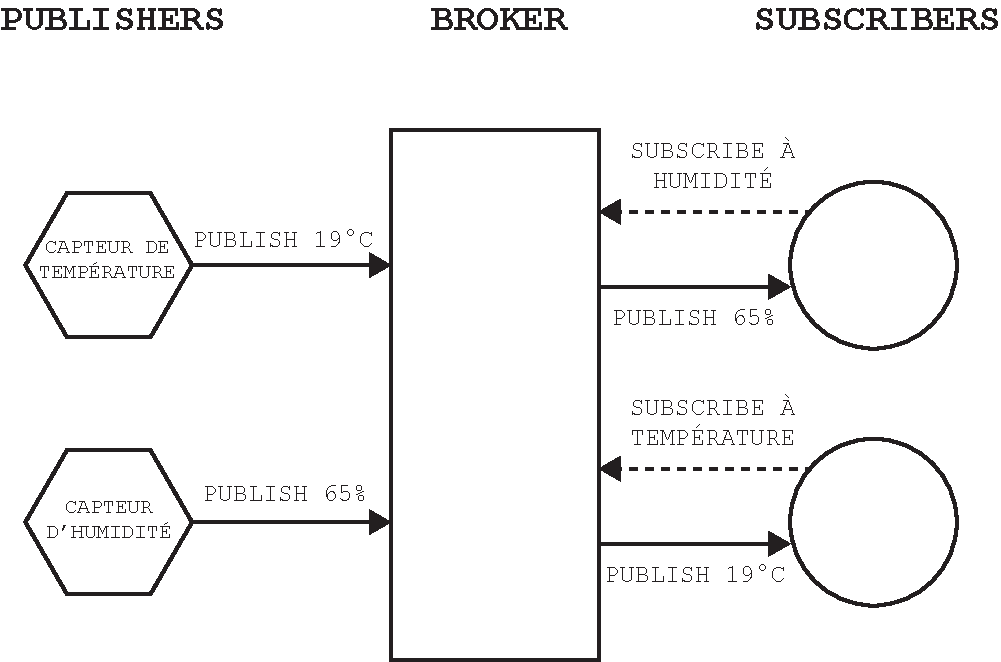
\includegraphics[width=10cm]{pub_sub.pdf}
        \caption{Illustration du fonctionnement du modèle \textit{publish/subscribe}.}
	\label{fig:pub_sub}
\end{figure}

Le modèle \textit{publish/subscribe} connaît de nombreuses implémentations parmi lesquelles il est possible de retrouver \ac{AMQP} \citep{Vinoski2006}, \ac{XMPP} \citep{Saint-Andre2011}, RabbitMQ \citep{Dossot2014} et ZéroMQ \citep{Hintjens2013}. Cependant, \ac{MQTT} est la plus connue d'entre elles \citep{Hunkeler2008}. En effet, grâce à sa portabilité \footnote{\url{https://github.com/mqtt/mqtt.github.io/wiki/libraries}} et sa faible consommation de ressources (débit, mémoire et consommation d'énergie), elle demeure une excellente une solution pour l'échange de données dans le domaine de l'\acs{IoT}, où la puissance des dispositifs reste encore relativement limitée. En plus des avantages offerts par le modèle \textit{publish/subscribe}, \acs{MQTT} propose la définition de trois différents niveaux de qualité de service (\acl{QoS} ou \acs{QoS}) : Le message est distribué une fois tout au plus, ou n'est pas distribué du tout ; le message est toujours distribué au moins une fois ou le message est toujours distribué une seule fois. Ceux-ci permettent donc une plus grande flexibilité en ce qui concerne le niveau de fiabilité requis par le système ; c'est-à-dire, la garantie que les messages sont, ou non, correctement envoyés et reçus. Aussi, dans son objectif de rester une solution légère, \acs{MQTT} permet d'avoir recours à une une option de sécurité relativement simple. Cette dernière consiste en une authentification des clients auprès du \textit{broker} \textit{via} un nom d'utilisateur et un mot de passe. Néanmoins, plusieurs couches de sécurité supplémentaires peuvent y être ajoutées (utilisation d'un réseau privé virtuel (\acl{VPN} ou \acs{VPN}), chiffrer les échanges de messages par \acs{SSL}/\acs{TLS}, \textit{etc.}) 

\subsection{Le cas spécifique du \acs{BLE}}

D'après le rapport publié par \cite{ON2017}, le \ac{BLE} serait la technologie de communication sans-fil la plus utilisée dans le domaine de l'\acs{IoT} et plus particulièrement des \textit{wearable devices}. De ce fait, la section \ref{subec:com_ble} ayant présenté les principales caractéristiques techniques de bas niveau pour cette technologie, il est désormais nécessaire d'en présenter le fonctionnement de haut niveau. En effet, la communication par \acl{BLE} oblige l'utilisation du protocole tel que défini par le standard. Par conséquent, l'implémentation d'un tout autre protocole de haut niveau déjà existant n'est pas possible avec cette technologie. Il apparaît donc nécessaire d'en comprendre le fonctionnement en détail.

Le protocole du \acs{BLE} est divisé en deux catégories: le contrôleur et l'hôte ; chacune admettant des sous-catégories parmi lesquelles il est possible de retrouver le \ac{GAP} et le \ac{GATT}. Le \acs{GAP} définit la topologie générale du réseau. En d'autres termes, si un dispositif Bluetooth est visible par d'autres, c'est par l'intermédiaire de ce profil. Il détermine comment les appareils peuvent, ou non, interagir entre eux. Le \acs{GATT}, quant à lui, décrit en détail la manière dont les données sont formatées, conditionnées et transférées selon les règles définies par l'\ac{ATT}. Pour communiquer avec le monde extérieur, un appareil \acs{BLE} peut se trouver en deux modes différents : le mode diffusion (figure \ref{fig:topo_broadcast}) ou le mode communication, qui correspond à une topologie étoile (figure \ref{fig:topo_star}). Ceux-ci sont définis dans les directives relatives au \acs{GAP}.

Dans le cas du mode diffusion, il est important de distinguer deux rôles que peuvent avoir les appareils \acs{BLE} : les diffuseurs et les observateurs. Pendant un intervalle de temps donné (l'intervalle de diffusion), le diffuseur est responsable d'annoncer publiquement des données. Si un observateur demande à récupérer les données annoncées par le diffuseur, ce dernier doit alors lui transmettre\textemdash sinon elles sont annoncées de nouveau dès lors que l'intervalle de diffusion est écoulé. Un nouveau cycle peut alors recommencer. En outre, il est important de noter qu'aucune connexion n'est établie entre un observateur et un diffuseur. Le fonctionnement de ce processus est illustré par la figure \ref{fig:ble_broadcast_process}.

À l'inverse du mode diffusion, deux appareils \acs{BLE}, lorsqu'ils sont en mode communication, doivent explicitement établir une connexion entre eux pour que des données puissent être échangées. Si un observateur demande une connexion à un diffuseur, le processus de diffusion s'arrête et il n'est plus possible d'obtenir les données qui étaient annoncées. Ce dernier adopte alors le rôle de périphérique et l'observateur devient le central. Un appareil \acs{BLE} ayant le rôle de périphérique ne peut se connecter qu'à un seul dispositif central à la fois, mais un central peut, quant à lui, être connecté à plusieurs périphériques. Cependant, la connexion peut être interrompue intentionnellement ou non (\textit{p. ex.} perte de l'alimentation), et ce, par n'importe quel dispositif. 

Dès lors que la connexion est établie, la communication entre le central et le périphérique peut commencer. Le dispositif qui demande les données joue alors le rôle de serveur \acs{GATT}. Puisque les rôles définis par le \acs{GAP} et le \acs{GATT} sont indépendants, le central et le périphérique peuvent tous deux devenir le serveur. Celui-ci est donc sollicité par le client \acs{GATT} qui lui envoie des requêtes. Le serveur \acs{GATT} indique un intervalle de connexion au client qui va alors essayer de se reconnecter après chaque délai pour récupérer de nouvelles données, si elles existent. Une représentation graphique du fonctionnement de ce processus est donnée en figure \ref{fig:ble_connect_process}. Les données sont transmises du serveur au client par une collection de services. Ceux-ci sont utilisés pour diviser les données en entités logiques et contiennent des blocs de données spécifiques qui sont les caractéristiques. Un service peut avoir une ou plusieurs caractéristiques et chaque service se distingue des autres au moyen d’un identifiant numérique unique (\acl{UUID} ou \acs{UUID}), qui peut être défini soit sur 16 bits (pour les services BLE officiels), soit sur 128 bits (pour les services personnalisés). Les caractéristiques sont elles aussi identifiées par un \acs{UUID} de 16 ou de 128 bits prédéfini. C'est via celles-ci que les informations sont échangées, car contrairement aux services, elles ne peuvent encapsuler qu'une unique donnée (\textit{p. ex.} une valeur binaire, un entier, un tableau de valeurs). 

\begin{figure}[H]
	\centering
	\subfloat[Échange de données en mode diffusion]{
		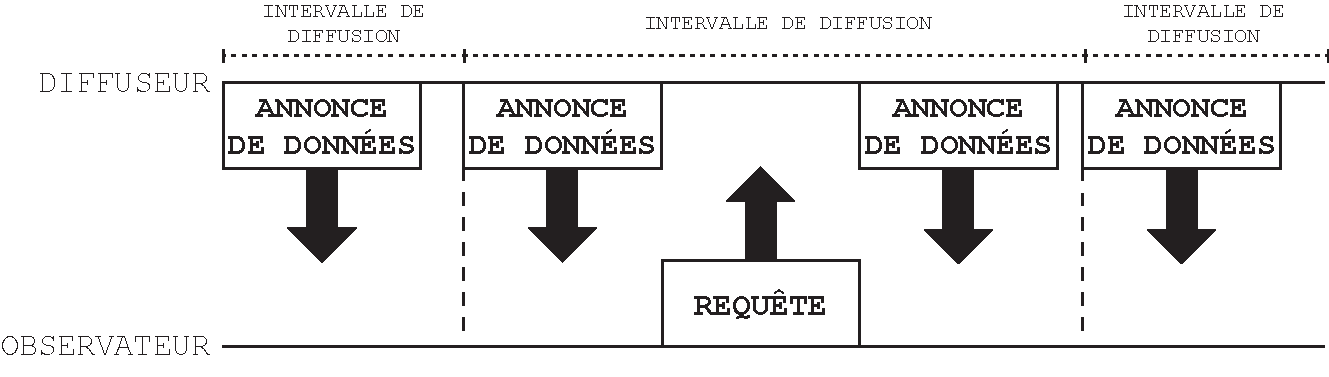
\includegraphics[width=.9\linewidth]{ble_broadcast_process.pdf}
		\label{fig:ble_broadcast_process}
    }
    \\[30pt]
	\subfloat[Échange de données en mode connexion]{
		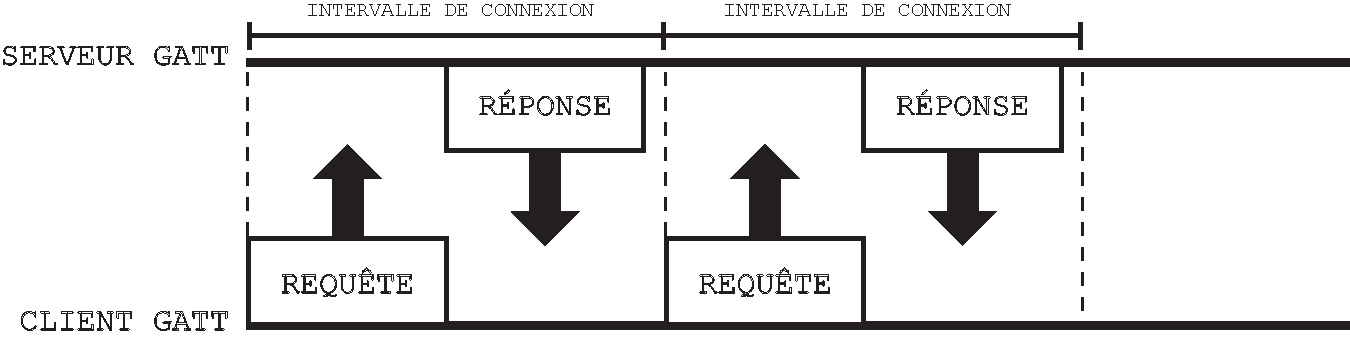
\includegraphics[width=.8\linewidth]{ble_connect_process.pdf}
		\label{fig:ble_connect_process}
	}
	\caption{Illustration du processus d'échange de données dans les deux modes de fonctionnement du \acs{BLE}, soit les modes diffusion et connexion.}
\end{figure}

\subsection{Les Services Web}

Les services web permettent à différentes applications de communiquer entre elles en fournissant une plateforme commune pour l'échange de données. Les requêtes et les réponses émises par les applications sont soumises à des standards. Parmi les plus populaires, il est possible de retrouver le protocole \ac{SOAP}, l'architecture \acl{REST} (\acs{REST}) et le protocole \acl{COAP} (\acs{COAP}). 

\subsubsection{Le protocole \ac{SOAP}}

Le protocole \ac{SOAP}, tout comme le modèle \textit{publish/subscribe}, est lui aussi utilisé dans les habitats intelligents depuis leur apparition. En effet, c'est principalement le cas de ceux ayant opté pour une architecture par composants et plus particulièrement \ac{OSGi} (comme Gator-tech \citep{Helal2005}), puisque cette technologie repose sur \ac{SOAP} pour tirer profit des services web. Depuis, de nombreux travaux se sont intéressés à l'interopérabilité des données ambiantes fournies par les habitats intelligents avec les données produites par les \textit{wearable devices} \citep{Perumal2008, Cubo2014, Diaz-Rodriguez2018}.

\ac{SOAP} est un protocole d'échange d'information structuré qui repose sur le langage \ac{XML}. Bien que ce dernier puisse être utilisé au-dessus de plusieurs autres protocoles tels que \ac{SMTP}, \ac{TCP} ou \ac{UDP}, il est majoritairement employé comme couche supérieure à \acl{HTTP} (\acs{HTTP}). Le protocole \ac{SOAP} appartient au modèle client/serveur et permet aussi bien l'appel de procédures respectant les propriétés ACID (Atomicité, Cohérence, Isolation et Durabilité), que le transfert d'informations. Dans ce dernier cas, un message est envoyé au serveur qui va alors traiter l'information et répondre au client.

Un message \ac{SOAP} est un document \ac{XML} qui contient un en-tête (\textit{header}) ainsi qu'un corps (\textit{body}), le tout encapsulé dans une enveloppe. Cette dernière indique que le document XML correspond à un message \ac{SOAP} et identifie le début ainsi que la fin de du message. L'en-tête, qui demeure facultatif, peut contenir différents attributs relatifs au message. Le corps, quant à lui obligatoire, contient les informations soit de la requête faite par le client, soit de la réponse du serveur, ainsi que des informations à propos des erreurs qui pourraient survenir. Les informations contenues dans le corps du message \ac{SOAP} sont organisées sous forme de blocs. La figure \ref{fig:soap_msg} montre un exemple d'échange de messages \ac{SOAP} à travers \ac{HTTP} qui permet d'obtenir la valeur du capteur cardiaque d'un dispositif quelconque.

L'avantage principal de l'utilisation de \ac{SOAP} comme méthode de communication est principalement la sécurité qu'offre ce protocole. En effet, ce dernier supporte le chiffrement \ac{SSL}, mais il permet également d'exploiter la spécification \textit{Web Services Security ou WS-Security} qui apporte des fonctionnalités de sécurité supplémentaires appréciées des entreprises. Cependant, il demeure un protocole peu flexible et relativement lourd et complexe à mettre en place.

\begin{figure}[H]
    \centering
	\subfloat[Requête \acs{SOAP}]{
		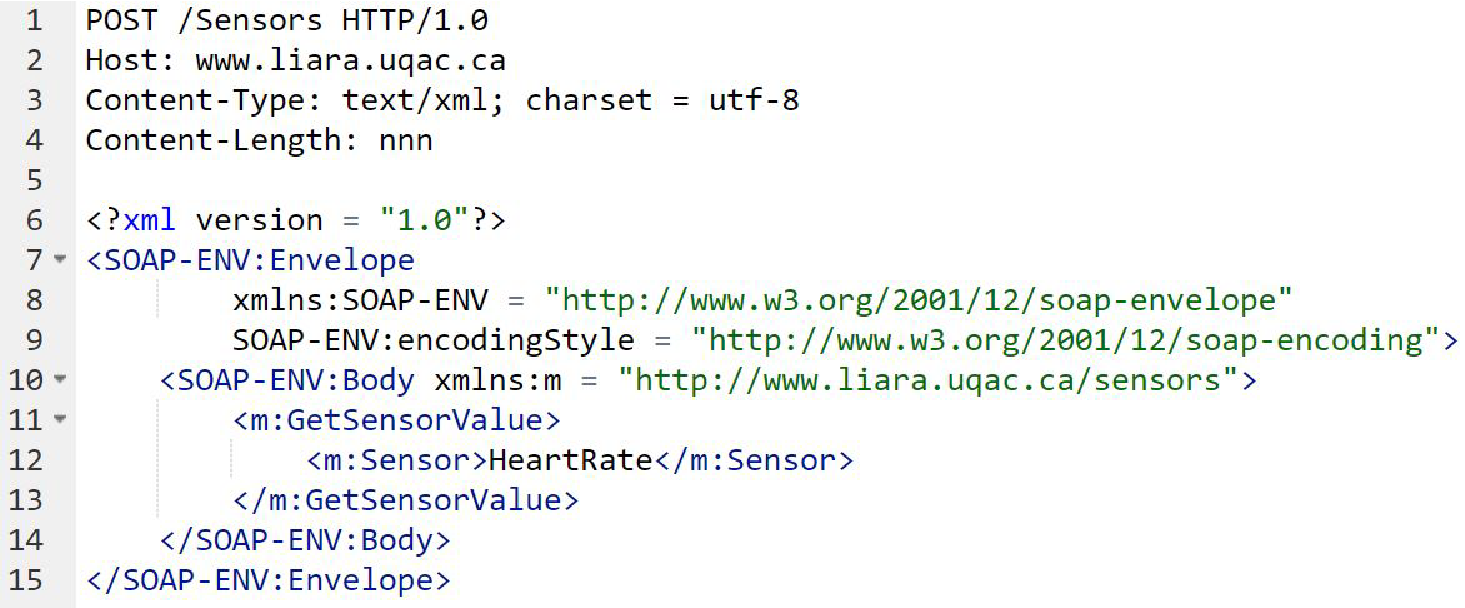
\includegraphics[width=.7\linewidth]{soap_req.pdf}
		\label{fig:soap_req}
    }
    \\[30pt]
	\subfloat[Réponse \acs{SOAP}]{
		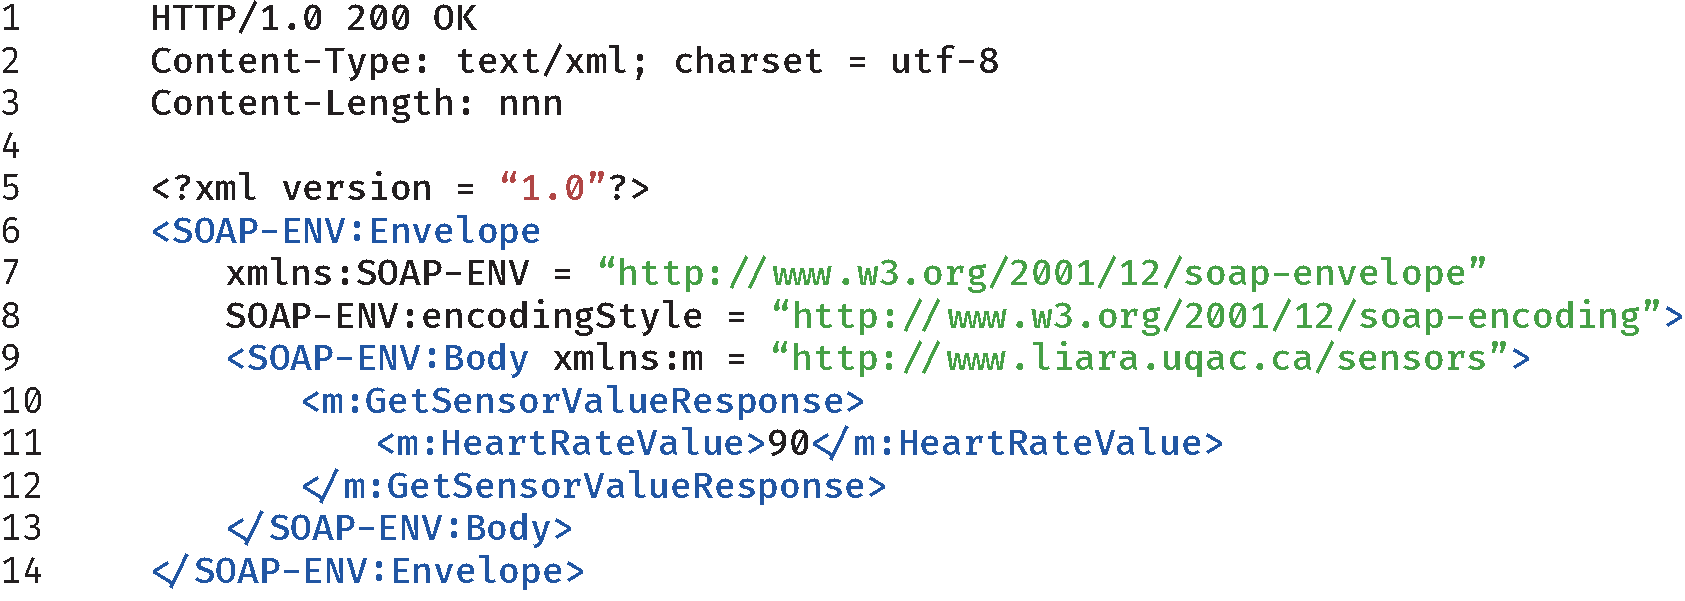
\includegraphics[width=.7\linewidth]{soap_res.pdf}
		\label{fig:soap_res}
    }
    \caption{Exemple d'un échange de messages \acs{SOAP} entre un client et un serveur pour obtenir la valeur du capteur cardiaque.}
    \label{fig:soap_msg}
\end{figure}

\subsubsection{L'architecture \ac{REST}}

Dès le début des années 2000, l'introduction des architectures de type \ac{REST} \citep{Fielding2000} a permis de remplacer petit à petit le protocole \ac{SOAP}, venant ainsi combler certaines de ses lacunes. Le principal avantage de ces architectures est leur indépendance vis-à-vis des protocoles existants. En effet, bien que les architectures \ac{REST} soient aussi majoritairement définies par-dessus \ac{HTTP}, elles pourraient tout autant l'être sur n'importe quel autre protocole\textemdash tant que celui-ci admet un schéma d'\ac{URI} normalisé. Tout comme pour \ac{SOAP}, les architectures \ac{REST} s'appuient sur le modèle de communication client/serveur. Cependant, à l'inverse de \ac{SOAP}, un service web \ac{REST} est sans état, c'est-à-dire que le serveur ne connaît pas l'état de chaque client entre les requêtes qu'il doit traiter. Ainsi, du point de vue du serveur, chaque requête est une entité distincte des autres. De plus, contrairement à \ac{SOAP}, qui impose le format d'échange de données en \ac{XML}, \ac{REST} accepte que les ressources, c'est-à-dire, les données échangées entre le client et le serveur, soient exprimées selon plusieurs formats de données tels que \ac{XML}, \ac{JSON} ou encore \ac{HTML}. Ceci garantit alors un meilleur support pour les clients.

Lorsqu'elle est définie sur \ac{HTTP}, une architecture \ac{REST} manipule ses ressources avec les différentes méthodes \ac{HTTP} ($GET$, $POST$, $PUT$, $DELETE$, $PATCH$). Ainsi, lorsqu'un client émet une requête indiquant l'opération qu'il souhaite effectuer sur une ressource donnée, la réponse transmise par le serveur contient les informations suivantes :

\begin{itemize}[label=\textbullet]
    \item 
        La version du protocole \ac{HTTP} utilisé pour le transport des données.
    \item 
        Le code \ac{HTTP} \citep{Fielding2014} qui indique l'état de la réponse.
    \item 
        Un en-tête qui fournit des informations à propos de l'échange d'information, par exemple, le format de donnée.
    \item 
        Le corps de la réponse qui peut contenir une ressource, un message d'erreur, \textit{etc.}
\end{itemize}

\noindent La figure \ref{fig:rest_get} illustre le processus de communication entre un client et un serveur dans une architecture \ac{REST} basée sur les méthodes \ac{HTTP}. Le client demande l'obtention de la valeur du capteur cardiaque d'un dispositif quelconque. Cette ressource est identifiée par l'\ac{URI} \url{http://liara.uqac.ca/sensors/health/1}. Puisque le serveur est capable de fournir la réponse attendue, et ce, sans erreur, le code \ac{HTTP} 200, ainsi que le nom et la valeur du capteur sont renvoyés au client au format \ac{JSON}, tel que précisé dans l'en-tête de la réponse.

\begin{figure}[H]
	\centering
	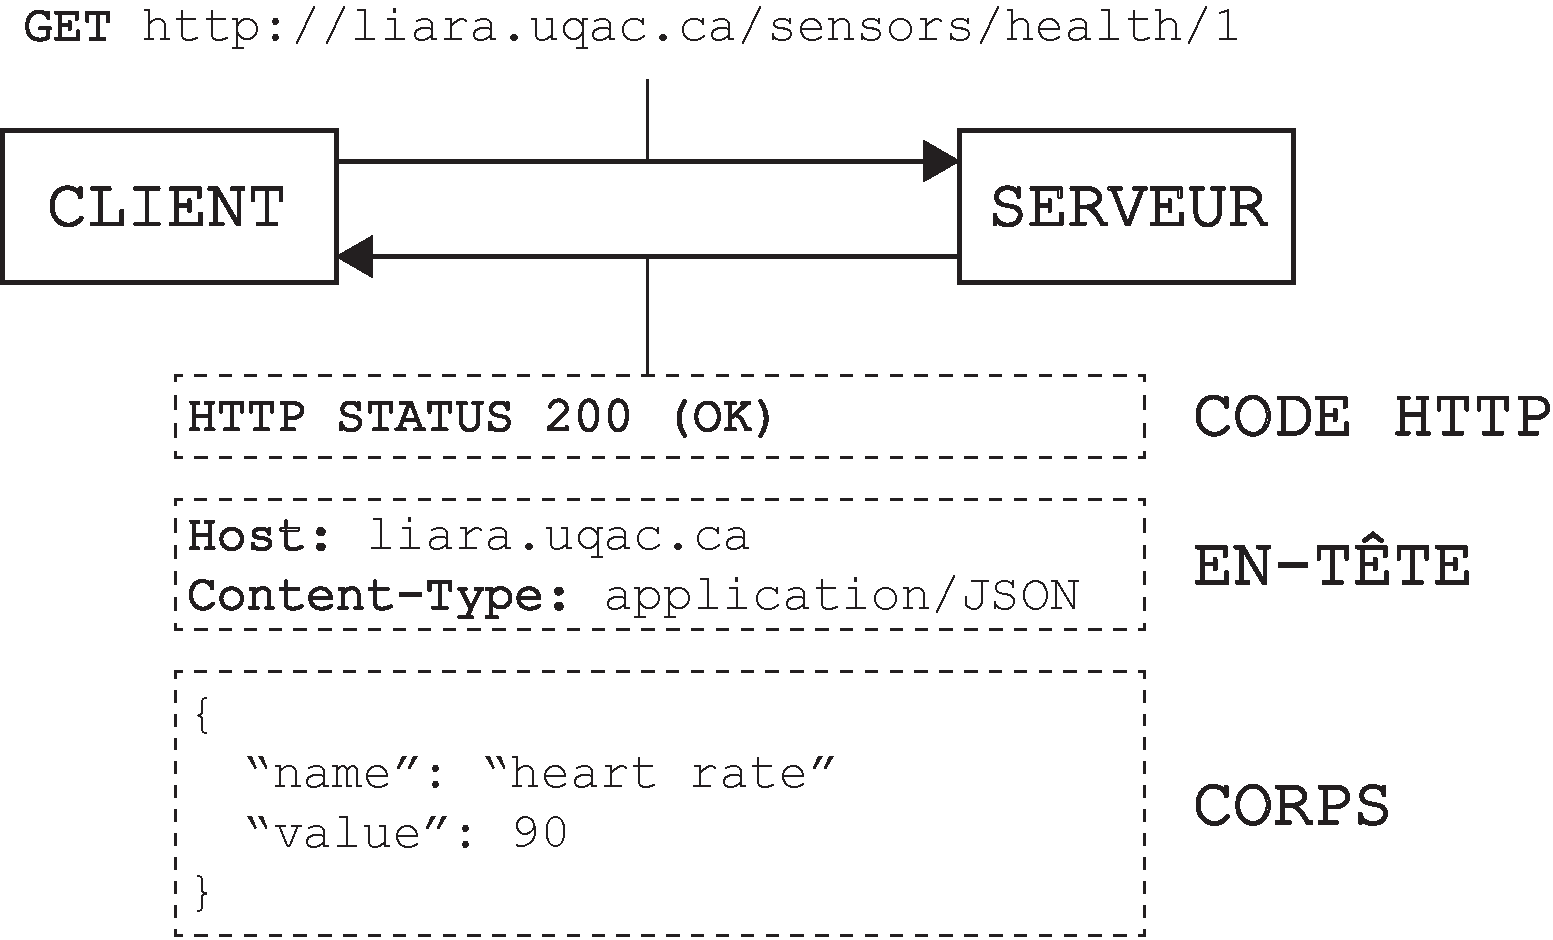
\includegraphics[width=10cm]{rest_get.pdf}
        \caption{Illustration d'un échange de messages entre un client et un serveur dans une architecture \ac{REST} basée sur \ac{HTTP} qui permet de récupérer la valeur d'un capteur cardiaque.}
	\label{fig:rest_get}
\end{figure}

\subsubsection{Le protocole \ac{COAP}}

Plus récemment, la recrudescence du nombre d'objets connectés et plus particulièrement de \textit{wearable devices} a fait émerger plusieurs problématiques inhérentes à la limitation de leurs ressources telles qu'une puissance de calcul restreinte, une faible quantité de mémoire ou encore une autonomie réduite. Cependant, la limitation de ces dispositifs implique également de nouvelles problématiques au regard du processus d'échange de données. En effet, malgré une meilleure efficacité qu'avec le protocole \ac{SOAP}, tant en termes de débit qu'en termes de consommation de ressources, l'exploitation des services web à travers une architecture \ac{REST} s'est parfois montrée inadaptée dans le contexte de l'\acs{IoT} \citep{Kovatsch2011}. En effet, lorsqu'une architecture \ac{REST} repose sur le protocole \ac{HTTP}, il a été observé qu'une grande fréquence de requêtes ne retournant qu'un nombre faible de données entraînait une surcharge réseau, principalement à cause des en-têtes \ac{HTTP} qui sont encodés en \ac{ASCII} \citep{Shelby2010}. Néanmoins ce cas de figure correspond au fonctionnement typique d'un réseau de capteurs sans-fil, où chaque message qui est envoyé correspond généralement à une seule mesure. Par conséquent, le protocole \ac{COAP} a été introduit par \cite{Shelby2014} afin de mieux répondre aux besoins des appareils ayant de fortes contraintes liées au débit, à la consommation et à la puissance de calcul. Malgré son jeune âge, plusieurs recherches se sont tournées vers une implantation de \ac{COAP} au sein des habitats intelligents \citep{Bergmann2012, Mainetti2015}. Par ailleurs, de récents travaux, comme celui introduit par \cite{Plantevin2017}, ont proposé de nouveaux protocoles de communication qui s'inspirent de la spécification de \ac{COAP}. Bien qu'ils soient encore très peu exploités, ceux-ci visent principalement à mieux intégrer l'\acs{IoT} au sein des habitats intelligents, puisqu'ils permettent d'optimiser davantage le processus d'échange de données. 

Pour mettre en place une architecture \ac{REST}, \ac{COAP} reprend plusieurs concepts de \ac{HTTP}, mais plusieurs optimisations ont été faites pour le rendre plus adapté aux systèmes embarqués. Premièrement, les échanges se font par des messages asynchrones qui comprennent des mécanismes de fiabilité optionnels comme que le protocole \ac{UDP}, qui est utilisé par défaut. En outre, les en-têtes sont compressés afin de réduire la complexité du décodage et les besoins en bande passante. Les messages \ac{COAP} contiennent les informations suivantes :

\begin{itemize}[label=\textbullet]
    \item 
        La version du protocole utilisée pour le transport des données.
    \item 
        Le type du message indique s'il s'agit, d'un message fiable qui exige un acquittement ($CON$), d'un message asynchrone qui n’a pas besoin d’être acquitté ($NON$), d'un message d’acquittement, c'est-à-dire, une réponse à une requête $CON$ ($ACK$), d'un message qui indique que le serveur a bien reçu la requête, mais qu'il n’a pas le contexte nécessaire pour fournir une réponse ($RST$).
    \item 
        Le nombre d'options transmises dans l'en-tête ($OC$).
    \item 
        Un code qui indique si le message est une requête, une réponse ou un message vide. Dans le cas d’une requête, la méthode utilisée est également précisée. Elles sont identiques aux méthodes \ac{HTTP}.
    \item 
        Un identifiant unique pour détecter les messages dupliqués et pour faire la correspondance entre un message $CON$ et son $ACK$ respectif.
    \item 
        Différentes options, par exemple, un paramètre pour définir la durée de validité des données transmises.
    \item 
        Les données en elles-mêmes.
\end{itemize}

\noindent La figure \ref{fig:coap_get} illustre le processus de communication entre un client et un serveur dans une architecture \ac{REST} basée sur \ac{COAP}. Le client demande l'obtention de la valeur du capteur cardiaque d'un dispositif quelconque où la requête et la ressource sont respectivement identifiées par le code $0x4d45$ et l'\ac{URI} \url{/sensors/health/hr}. Le serveur transmet alors immédiatement le message $ACK$ ainsi que la valeur du capteur.

\begin{figure}[H]
	\centering
	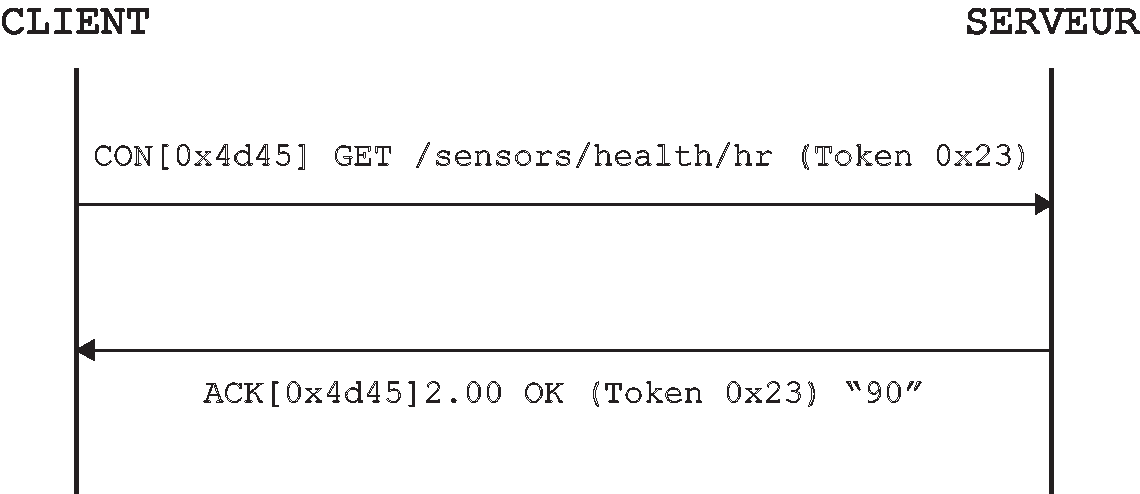
\includegraphics[width=10cm]{coap_get.pdf}
        \caption{Illustration d'un échange de messages entre un client et un serveur dans une architecture \ac{REST} basée sur \ac{COAP} qui permet de récupérer la valeur d'un capteur cardiaque.}
	\label{fig:coap_get}
\end{figure}

Puisque la différence majeure entre \ac{COAP} et \ac{HTTP} réside dans l'utilisation du protocole \ac{UDP}, ceci lui permet de supporter le \textit{multicast}, ce qui n'est pas le cas du protocole \ac{HTTP}. Aussi, comme \ac{COAP} est principalement conçu pour l'\acs{IoT}, ce protocole se base exclusivement sur IPv6 avec 6LoWPAN (\textit{IPv6 Low power Wireless Personal Area Networks}), lui permettant de mieux prendre en compte le volume d'entités qui composent un réseau de capteurs sans-fil. Enfin, il permet de mettre en place aussi bien un modèle client/serveur, tel qu'illustré dans l'exemple précédent, qu'un modèle \textit{publish/subscribe} à l'instar du protocole \ac{MQTT}. 

%%%
% \section{Les cas d'utilisation}
% \subsection{Surveillance de la santé}
% \subsection{Détection et prévention des chutes}
% \subsection{Reconnaissance d'activités}
%%%
\section{Conclusion}
 
Dans un premier temps, ce chapitre s'est intéressé à la couche matérielle qui compose les \textit{wearable devices}. Les capteurs les plus adéquats pour être embarqués dans ce type de dispositifs ont été regroupés en différentes catégories qui sont, les capteurs de mouvement, les capteurs physiologiques, les capteurs de courbure et de force ainsi que les capteurs environnementaux. Bien qu'il en existe beaucoup d'autres, ce chapitre a montré que ceux-ci demeurent les plus utilisés dans divers domaines de recherche tels que la réhabilitation, la surveillance de la santé et surtout dans la reconnaissance de gestes et d'activités. 

Ensuite, ce chapitre a présenté les technologies de communication sans-fil actuellement employées par les \textit{wearable devices}, mais également les futures évolutions de chacune d'elles. Il est apparu que toutes s'inscrivent dans l'optique de mieux prendre en compte le nombre grandissant d'objets connectés, plus particulièrement en ce qui concerne leur limitation énergétique. De plus, en ne considérant que les capacités actuelles de chaque technologie, ce chapitre a proposé un comparatif de leurs différences en termes de capacité de portée, débit et robustesse. Ceci a permis de conclure que le choix de la technologie à adopter dans le processus de conception de \textit{wearable devices} en fonction des contraintes liées à l’utilisation qui doit en être faite.

Enfin, dans sa dernière partie, ce troisième chapitre a exposé les différents protocoles et architecture de haut niveau permettant aux \textit{wearable devices} d'échanger leurs données avec d'autres entités qui composent un réseau (capteurs intelligents, serveur central, \textit{etc.}). Ainsi, dans les travaux sur les habitats intelligents et leurs évolutions pour y intégrer l'\acs{IoT}, deux principaux modèles pour l'échange de données ont été retenus. Le premier est le modèle \textit{publish/subscribe} et plus particulièrement le protocole \acs{MQTT}. Le second concerne le modèle client/serveur, plus traditionnel. Bien qu'il admette un fonctionnement particulier, le cas du \acs{BLE} s'appuie fortement sur ce deuxième modèle. De plus, des méthodes plus récentes issues du web social comme la consommation de services web appartiennent également à un modèle client/serveur. Pour tirer profit des services web, plusieurs technologies comme le protocole \acs{SOAP} ou les architectures \acs{REST} ont été mises en place au sein des infrastructures d'habitats intelligents. Cependant, certaines limitations quant à l'intégration de l'\acs{IoT} ont pu être observées. Pour combler ces problématiques, de nouvelles implémentations comme le protocole \acs{COAP} ont été mises en place dans ces habitats. 
\let\cleardoublepage\clearpage
\chapter{Méthodologie}
\label{chap:4}

Dans les chapitres précédents, les différentes architectures d'habitats intelligents ainsi que les efforts mis en place pour y intégrer les \textit{wearable devices} ont été étudiés. De plus, les technologies aussi bien matérielles que logicielles spécifiques à ces dispositifs qui permettent de réaliser le processus d'apprentissage ont été détaillées et les problématiques qui y sont rattachées ont été exposées. 

Ainsi, ce projet propose, dans un premier temps, de développer de nouveaux types de \textit{wearable devices} dans l'optique d'améliorer l'assistance déjà offerte par les habitats intelligents. En effet, il semble que les technologies de reconnaissance existantes puissent être améliorées par de nouveaux systèmes faisant intervenir des \textit{wearable devices} qui agiraient alors en tant que solutions complémentaires. Dans un second temps, l'objectif de ce projet est de proposer un outil capable d'uniformiser les précédents travaux qui concernent l'assistance au sein des habitats intelligents avec des \textit{wearable devices}. En effet, grâce aux chapitres précédents, il est apparu que chaque solution existante impliquant ce type de dispositifs admet un fonctionnement entièrement autonome, c'est-à-dire mal intégré à l'environnement dans lequel il est utilisé (les habitats intelligents). De plus, pour réaliser le processus d'apprentissage, bien que la majorité des travaux incluent des composantes logicielles identiques, les données qui y sont exploitées n'appartiennent à aucune standardisation. Ainsi, l'idée est de proposer un outil simple à intégrer au sein d'un habitat intelligent et qui offrira la possibilité à tous les \textit{wearable devices} de fonctionner ensemble, mais également en combinaison avec les technologies \og statiques \fg de l'habitat.  

Ce quatrième et dernier chapitre va commencer par présenter l'infrastructure qui servira de base pour mener à bien ce projet de recherche qui s'articule en deux phases principales, chacune répondant aux différentes lacunes qui ont pu être observées dans les chapitres précédents. 

\section{Infrastructure : le \acs{LIARA}}

Ce projet de recherche va être réalisé grâce aux infrastructures offertes au \acs{LIARA}. Situé au sein de l'\ac{UQAC}, ce laboratoire offre un habitat intelligent complet d’une surface de cent mètres carrés dans lequel un grand volume de capteurs et d'effecteurs ambiant de types totalement différents y ont été intégrés. Le \acs{LIARA} est montré en figure \ref{fig:liara} En effet, il est question ici d’une centaine de capteurs tels que des contacteurs électromagnétiques, des thermomètres, des antennes et tags \acs{RFID}, des capteurs de luminosité, de débit d’eau et même de consommation électrique. De plus, le laboratoire offre également des effecteurs tels que des lumières contrôlées, des écrans et un système de haut-parleurs IP. L’intégralité de ces capteurs et effecteurs est connectée à une même base de données pour faciliter l’accès aux données et l’interaction avec l’infrastructure. Par exemple, des tapis de pression situés respectivement devant le lit et devant le lavabo de la salle de bain permettent de déterminer la présence d'une personne. De plus, des contacteurs électromagnétiques sont placés sur les placards et portes pour surveiller leurs ouvertures et fermetures. Enfin, les huit antennes \acs{RFID} permettent d'évaluer la position des objets qui sont équipés de tags et leur position est indiquée sur un écran qui affiche un plan du laboratoire.

\begin{figure}[H]
	\centering
	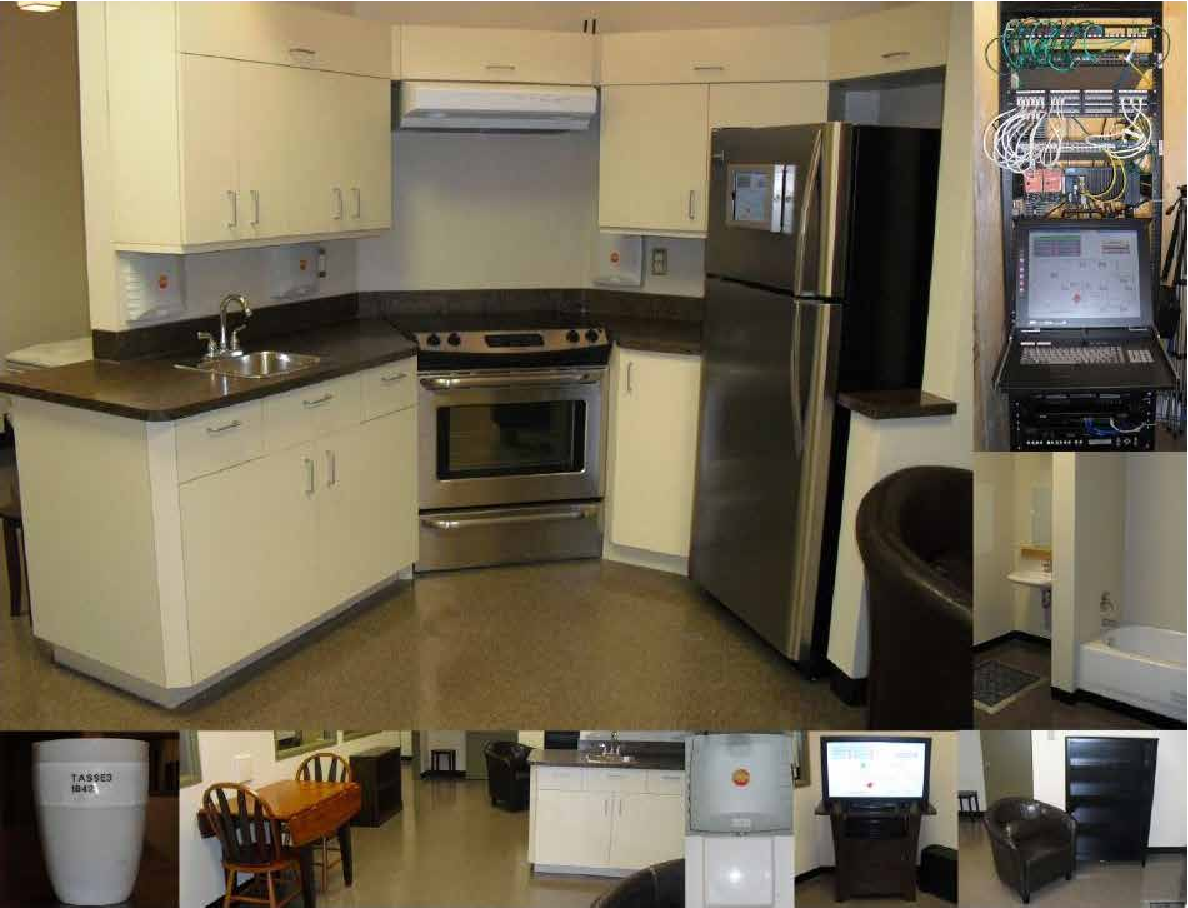
\includegraphics[width=.9\textwidth]{liara.pdf}
        \caption{Ensemble des pièces qui compose le \acs{LIARA}.}
	\label{fig:liara}
\end{figure}

Cette infrastructure constituera donc le cadre principal de toutes les expérimentations qui seront requises pour valider chacune des deux phases principales qui composent ce projet de recherche. 

\section{Phase I : avancements dans l'exploitation des \textit{wearable devices}}

Dans un premier temps, pour répondre à la première question énoncée en section \ref{sec:def_proj}, ce projet de recherche propose de s'intéresser à la conception de nouveaux \textit{wearable devices}. Ces derniers ont souvent été utilisés dans de nombreux domaines tels que la reconnaissance de gestes et d'activités, la réhabilitation ainsi que pour la surveillance de la santé au sein des habitats intelligents \citep{Khan2016, Davis2016, Chapron2018}. Cependant, certaines pistes qui permettraient d'améliorer l'assistance des résidents d'habitats intelligents semblent actuellement encore inexplorées. 

En ce sens, le premier \textit{wearable device} qui sera proposé dans ce projet de recherche va permettre de reconnaître les différents types de sols. Cette première contribution fera intervenir plusieurs algorithmes et technologies qui ont été présentés dans les chapitres précédents. En effet, une telle reconnaissance sera réalisée sur des données inertielles générées par le dispositif qui sera porté à différents endroits par un utilisateur. Cette idée est principalement issue du domaine de la robotique, où plusieurs travaux ont proposé cette idée pour améliorer la démarche des robots \citep{Bibuli2007a, Weiss2007a, Kertesz2016a}. Plus récemment, cette idée a également été expérimentée par \cite{Otis2016a} qui ont proposé l'utilisation d'une chaussure embarquant un accéléromètre. Cette dernière, capable de reconnaître les différents types de sols sur lesquels ses utilisateurs marchaient, avait pour objectif principal de déterminer un niveau de risque de chute et, en cas de danger, prévenir les marcheurs par une vibration sous le pied. 

Les objectifs visés par cette première contribution s'intègrent parfaitement dans l'optique d'assistance au sein d'un habitat intelligent, car ceux-ci peuvent comporter différents types de sols qui peuvent constituer des dangers ou causer de la peur chez les résidents. Par exemple, il est possible de mentionner les tapis, le carrelage mouillé dans la salle de bain ou encore les marches. Par conséquent, il demeure assez simple de voir comment une telle reconnaissance pourrait être intégrée à un \textit{wearable device} existant plus complet, déjà utilisé pour l'assistance au sein d'un habitat intelligent. De plus, l'idée de reconnaître des types de sol grâce à un \textit{wearable device} pourrait être adaptée à d'autres domaines comme celui du sport où ces dispositifs sont très largement utilisés \citep{Nielsen2014b}.

La seconde contribution visant à faire avancer l'exploitation des \textit{wearable devices} au sein des habitats intelligents concerne la conception d'une carte intelligente pour la sécurité d'accès et la personnalisation de ces habitats. En effet, chaque habitant étant unique, il possède nécessairement des habitudes et des goûts qui lui sont propres, comme la température d'une pièce. Il convient donc de trouver un moyen d'adapter la maison intelligente, non seulement à la maladie de son habitant, mais aussi aux préférences de celui-ci. Pour ce faire, ce projet de recherche proposera un second dispositif capable d'utiliser la démarche, qui est une donnée biométrique reconnue, pour identifier son porteur. Grâce à la combinaison de la reconnaissance de la démarche ainsi qu'à un tag \acs{NFC} embarqué directement dans la carte, l'accès à l'habitat intelligent pourra être sécurisé efficacement. De plus, ce dispositif pourra, après cette première vérification, aviser l'environnement des préférences de son porteur.

\section{Phase II : interopérabilité des \textit{wearable devices} au sein des habitats intelligents}

Dans un second temps, ce projet va proposer un système permettant de mieux intégrer les \textit{wearable devices} dans les habitats intelligents. En effet, les différentes architectures qui ont été proposées pour la conception de ces habitats n’ont pas été initialement prévues pour accueillir ces dispositifs. Par conséquent, ceux-ci se retrouvent très mal, voir nullement intégrés au sein des habitats intelligents. 

Ainsi, pour répondre aux questions \ref{question:2} et \ref{question:3} de la définition de ce projet de thèse, cette seconde phase a pour but de concevoir un outil capable de gérer à la fois les capteurs ambiants d'un habitat intelligent et les \textit{wearable devices} qui y sont utilisés. Ceci permettra alors de mettre en place une reconnaissance basée sur la fusion de ces sources de données diverses. Cet outil adoptera une conception modulaire permettant d'y ajouter des fonctionnalités supplémentaires, par exemple, un nouvel algorithme d'apprentissage. Aussi, il offrira la possibilité de réutiliser les différentes techniques qui composent le processus de reconnaissance d'activités détaillées dans le chapitre \ref{chap:2}. De ce fait, et en considérant une utilisation dans un cadre académique, cela simplifiera le développement de futurs dispositifs ainsi que les procédures expérimentales. Enfin, pour vérifier l'apport quant à une meilleure intégration des \textit{wearable devices} au sein des habitats intelligents, l'outil proposé devra, au minimum, être facilement déployable dans le type d'architecture du \acs{LIARA}.

\section{Planification}

Cette section présente la planification prévisionnelle donnée sous forme de diagramme GANTT par la figure \ref{fig:planification} expose un estimé du temps nécessaire à la réalisation de chaque tâche pour atteindre les objectifs de ce projet de recherche. 

\begin{figure}[H]
    \begin{sideways}
     \begin{minipage}{.7\textheight}
        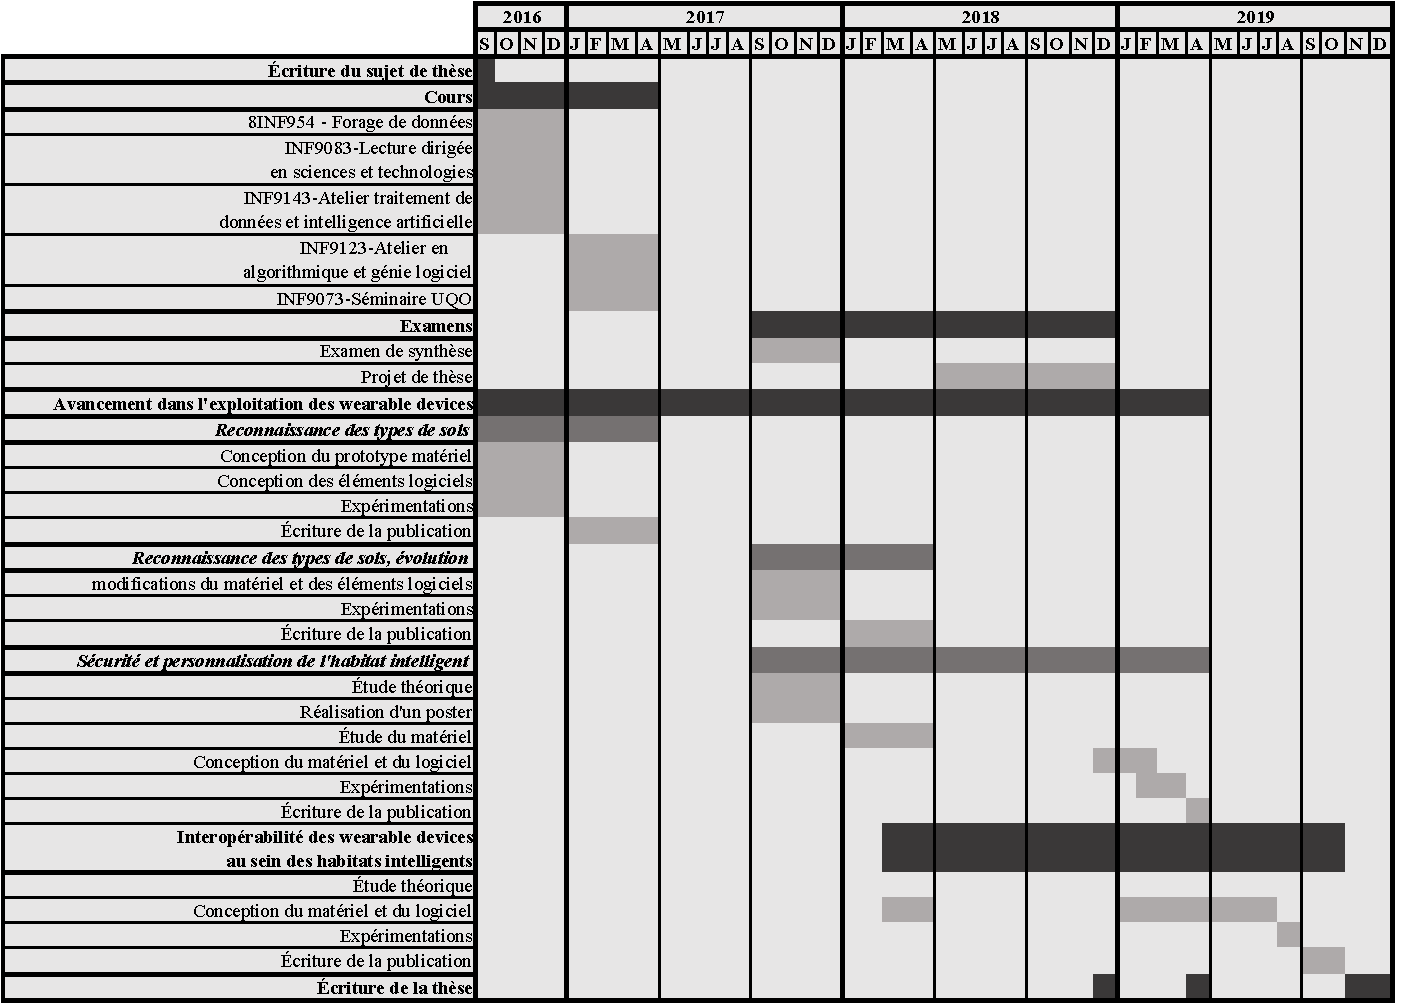
\includegraphics[width=\textwidth]{planification.pdf}
     \end{minipage}
    \end{sideways}
    \centering
    \caption{Planification de la thèse.}
    \label{fig:planification}
\end{figure}

\let\cleardoublepage\clearpage
\chapter{Une architecture d'habitats intelligents distribuée}
\label{chap:5}

Grâce aux chapitres précédents, il a été vu que les \textit{wearable devices} sont de plus en plus utilisés dans le processus de reconnaissance d'activités au sein des habitats intelligents. Aussi, ces dispositifs ont également été employés dans l'objectif de répondre à plusieurs autres problématiques concrètes, comme la méthode de reconnaissance des types de sols qui a été présentée au chapitre \ref{chap:4}, qui sont relatives à l'assistance des résidents de ces habitats, au sens large. Néanmoins, l'engouement croissant pour ces dispositifs a permis d'identifier plusieurs problématiques quant à leur utilisation dans ce contexte de recherche particulier. En effet, nous avons été en mesure d'identifier que la plupart des différentes architectures d'habitats intelligents qui ont été proposées antérieurement n'ont pas été développées dans une optique évolutive. Lorsqu'une intégration matérielle des \textit{wearable device} s'est montré facilement réalisable, comme dans l'architecture CASAS \citep{Cook2013}, cela était au détriment de la fiabilité du processus de la reconnaissance d'activités principalement affectée par une conception d'habitat admettant plusieurs points de défaillance. Par conséquent, la principale question de recherche qui est traitée dans ce chapitre est : \textit{\og comment faire évoluer les architectures de maisons intelligentes pour leur permettre de mieux s'adapter aux divers types de capteurs (ambiants et \textit{wearable devices}) tout en garantissant un excellent niveau de fiabilité dans l'accomplissement des différents processus d'apprentissage ? \fg}.

Pour répondre à cette question, le travail présenté dans ce chapitre propose un type différent d'architecture de maisons intelligentes. Cette implémentation a été développée en s'inspirant des architectures de \textit{cloud} privé sur site qui disposent de nombreux mécanismes qui permettent de s'assurer que l'infrastructure matérielle demeure hautement disponible, ceci dans le but de garantir à la fois un excellent niveau de fiabilité, mais également une évolutivité notoire. Ainsi, cette architecture vise à résoudre la plupart des problèmes identifiés au sein des habitats précédemment proposés sans qu'il soit nécessaire de remplacer leur structure matérielle dans leur intégralité. En effet, l'architecture présentée dans ce chapitre a été pensée pour à la fois être déployée en l'état, ou pour s'intégrer à celles existantes, remplaçant ainsi les entités centrales des architectures monolithiques.

La suite de ce chapitre comporte une première section qui présente en détail l'architecture d'habitats intelligents proposée. Ensuite, les expérimentations sont décrites dans une seconde section. Finalement, ce chapitre propose une discussion des observations réalisées et dresse une conclusion quant à ce second travail, dans une dernière partie.

% Il a été vu, dans les chapitres précédents qu'au fil des ans, diverses architectures de maisons intelligentes ont été proposées et mises en place au sein de laboratoires ou dans de réelles habitations pour mener des activités de recherche \citep{DJCook2003,Helal2005,Giroux2009,Cook2013,Bouchard2014,Lago2017,Plantevin2018}. Ces travaux se sont particulièrement intéressés à l'utilisation de capteurs, d'effecteurs et de techniques d'apprentissage machine pour la mise en application de l'\acl{IAm} comme méthode empirique afin de soutenir l'autonomie des personnes âgées et le suivi de la santé. Cependant, bien que chacun de ces travaux se distingue des autres, tous proposent différentes méthodes pour résoudre le problème principal de la reconnaissance d'activités. Les avantages et les inconvénients de chaque architecture d'habitats intelligents ont déjà été discutés dans cette thèse et le principal problème qui a été identifié réside dans le manque de fiabilité et l'évolutivité de ces implémentations. En effet, la plupart des architectures admettent au moins un point de défaillance, principalement à cause de leur implémentation centralisée, ou monolithique. Néanmoins, \cite{Plantevin2018} ont adressé cette problématique en introduisant un nouveau type d'architecture basée sur l'utilisation de transducteurs intelligents distribués. Cependant, bien que cette implémentation ait été pensée pour être une architecture de maisons intelligentes prête à l'emploi en situation réelle d'utilisation, sa conception ne semble pas suffisamment adaptée aux environnements de recherche. En effet, la simplicité de mise en place de nouvelles méthodes pour la reconnaissance d'activités et de nouveaux protocoles expérimentaux semble avoir été oubliés dans cette implémentation.

% Par ailleurs, dans la comparaison des différentes architectures de maisons intelligentes proposées au Chapitre \ref{chap:2}, le principal inconvénient des solutions existantes qui a été identifié concerne leur manque de flexibilité quant à l'intégration de nouveaux matériels et plus spécifiquement, les \textit{wearable devices}. En effet, pour réaliser la reconnaissance d'activités, la plupart des méthodes proposées avec ces dispositifs sont des applications complètes. La plupart du temps, les différents processus qui composent la reconnaissance sont encapsulés au sein d'un unique composant logiciel immuable. Il devient donc difficile de les modifier. De plus, le fait de disposer d'une unique application ne favorise pas la réutilisation de certains mécanismes communs à plusieurs méthodes. Ceux-ci doivent donc généralement être soit développés à nouveau, soit adaptés afin de pouvoir supporter des modifications dans la méthode proposée. De surcroît, l'exploitation de ce genre d'application \og prête à l'emploi \fg est, la plupart du temps, complexifiée. En effet, selon les dépendances, le langage de programmation et la plateforme, elles peuvent être difficiles à adapter et à déployer d'un environnement à un autre (\textit{p. ex.} entre deux laboratoires de recherche différents).

% Ainsi, ce travail présente un autre type d'architecture de maisons intelligentes qui se veut fiable et évolutive dont l'implémentation est inspirée des architectures de \textit{cloud} privées sur site. Cette architecture vise à résoudre la plupart des problèmes identifiés au sein des implémentations précédemment proposées sans qu'il soit nécessaire de remplacer leur structure au complet. En effet, l'implémentation présentée dans ce chapitre a été pensée pour à la fois être déployée en l'état, ou pour s'intégrer aux architectures existantes, remplaçant ainsi les entités centrales des architectures monolithiques. L'objectif principal de cette implémentation est alors de pouvoir y déployer facilement de nouveaux composants logiciels expérimentaux indépendamment des différences dans leur conception, tant en termes de langages de programmation que de librairies requises ou de plateforme supportées. Ceci dans le but de favoriser l'interopérabilité entre les différents processus, leur réutilisation ainsi que leur mise à l'échelle vis-à-vis de la quantité de ressources requise.

% La suite de ce chapitre comporte une première section qui présente en détail l'architecture d'habitats intelligents proposée. Ensuite, les expérimentations sont décrites dans une seconde section. Finalement, ce chapitre propose une discussion des observations réalisées et dresse une conclusion quand à ce second travail, dans une dernière partie.

\section{Architecture Proposée}

Bien que l'architecture introduite dans ce chapitre ait été conçue pour être compatible avec la majorité des architectures de maisons intelligentes présentes dans la littérature, celle-ci peut surtout être considérée comme une évolution du travail proposé par \cite{Plantevin2018}. En effet, puisque les auteurs ont concentré leurs efforts sur une intégration matérielle uniforme des transducteurs (capteurs et effecteurs), ils ont amorcé les mêmes perspectives d'amélioration des habitats intelligents existants en se penchant principalement sur les capteurs ambiants. Par conséquent, cette thèse ne prendra pas en considération ce type de capteurs, mais va plutôt traiter exclusivement des \textit{wearable devices}. De plus, l'objectif principal de ce travail est d'aller plus loin dans l'idée de rendre ces architectures plus fiables, mais aussi plus flexibles et évolutives. Pour ce faire, ce chapitre présente une implémentation qui repose sur l'utilisation des microservices plutôt qu'une approche monolithique.

\subsection{Microservices}

Les architectures de microservices sont récemment apparues comme un nouveau paradigme pour la programmation d'applications \citep{Dragoni2017} et dont l'origine se base sur le concept d'\ac{AOS} \citep{MacKenzie2006}. Comme le montre la figure \ref{fig:mono_micro}, cette approche suggère de diviser une application en un ensemble de services plus petits, indépendants et interconnectés. En comparaison aux applications monolithiques, où tous les composants logiciels se trouvent dans une seule instance, les services exécutent des fonctions plus détaillées et précises. Bien que les architectures monolithiques soient simples à implémenter, les architectures de microservices présentent, elles aussi, différents avantages. La première concerne l'\emph{agilité} des microservices. En effet, puisque les applications sont fragmentées au niveau le plus élémentaire de leurs fonctionnalités, chaque service devient individuellement plus facile à maintenir et beaucoup plus rapide à développer et à déployer. Le second avantage principal demeure la \emph{réutilisabilité}. Les microservices permettent aux développeurs de créer des applications en utilisant certains fragments déjà existants. De plus, la barrière entre les technologies (\textit{p. ex.} les langages de programmation) est réduite puisque les services fonctionnent de manière indépendante. En ce sens, cet \emph{agnosticisme technologique} permet d'obtenir des applications hétérogènes du point de vue des technologies dans leur conception. Par ailleurs, un autre avantage offert par les architectures de microservices concerne la mise à l'échelle des différents composants à mesure que la demande pour une application augmente. En cas de forte demande ponctuelle, il est possible soit d'augmenter la quantité de ressources allouées, soit d'augmenter le nombre d'instances pour les services les plus impactés, plutôt que pour l'intégralité de l'application. Il s'agit respectivement de l'\emph{extensibilité dynamique horizontale} et de l'\emph{extensibilité dynamique verticale}. Enfin, puisque les composants d'une application dans une architecture de microservices sont généralement distribués, l'application est en mesure de supporter les pannes au niveau des services qui la composent. En effet, lorsqu'un service est en panne, la fonctionnalité dont il est responsable devient inopérante, mais le fonctionnement du reste de l'application n'est pas altéré. De plus, il est possible de mettre en place différents mécanismes pour remédier aux défaillances inattendues afin d'augmenter la résilience et la \emph{fiabilité} de l'ensemble du système.

\begin{figure}[H]
	\centering
	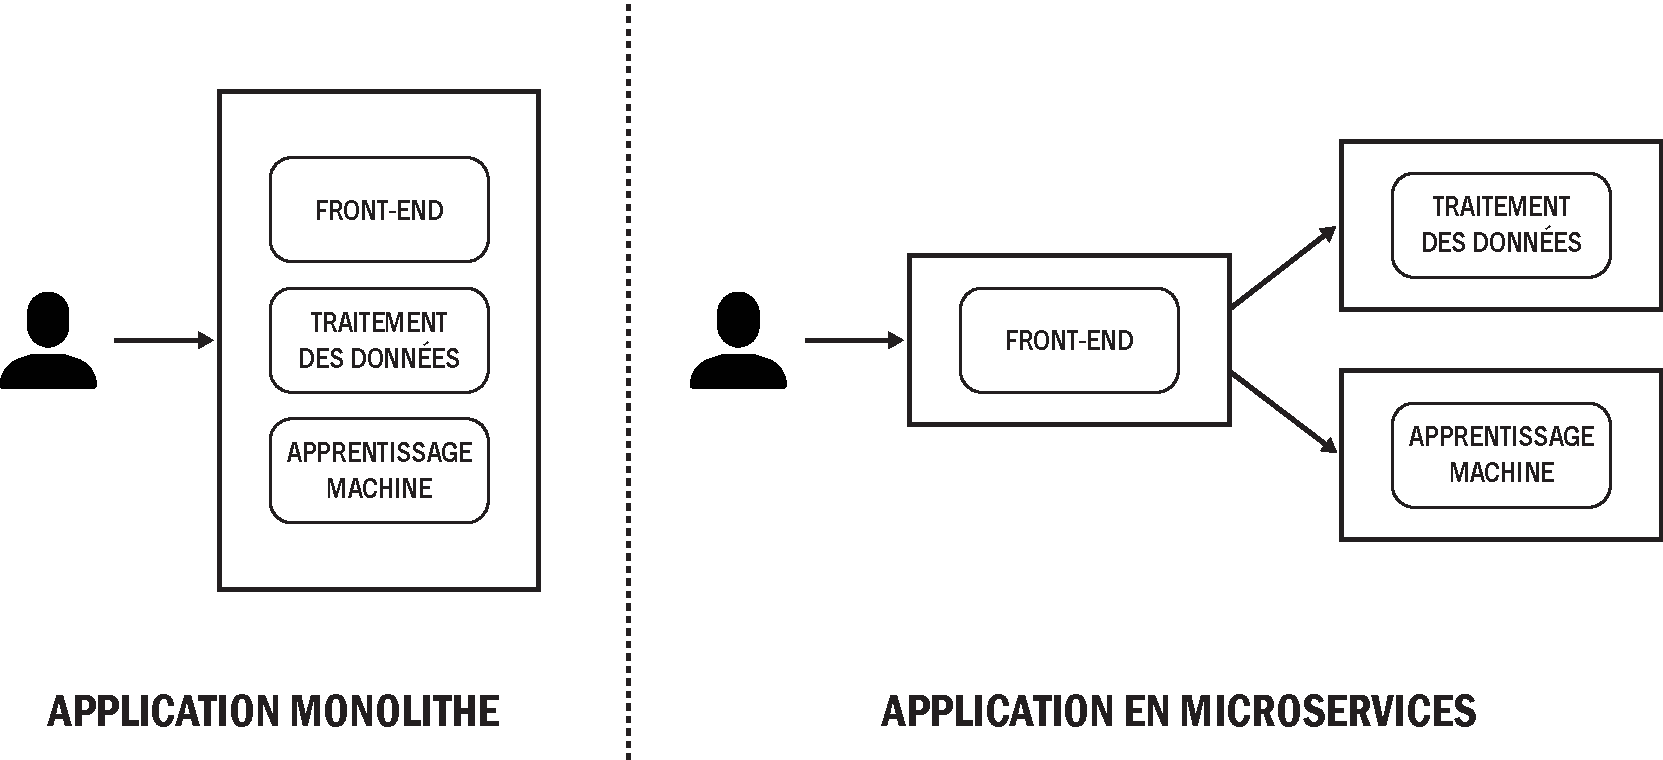
\includegraphics[width=.8\linewidth]{chapter5/mono_micro.pdf}
		\caption{Comparaison entre les architectures monolithiques et de microservices selon un exemple d'application qui vise à résoudre un problème d'apprentissage machine par le biais d'une interface graphique.}
	\label{fig:mono_micro}
\end{figure}

Actuellement, il existe de nombreuses façons de mettre en place une architecture de microservices, la plus courante étant l'utilisation d'outils de virtualisation tels que les machines virtuelles (\acsp{VM}) traditionnelles, les conteneurs ou les conteneurs à l'intérieur de \acsp{VM}. La figure \ref{fig:containers_vms} fournit une représentation graphique de ces trois différentes implémentations. Même si le choix de la méthode de virtualisation n'affecte pas les possibilités offertes par les architectures de microservices, il existe des différences significatives entre l'utilisation de \acsp{VM} traditionnelles et les conteneurs qu'il semble important de détailler. La principale différence réside dans le fait que les conteneurs proposent une virtualisation au niveau du système d'exploitation alors que les \acsp{VM} offrent une virtualisation au niveau du matériel. En ce qui concerne les \acsp{VM}, l'hyperviseur permet de cloisonner des portions du matériel. En effet, son rôle est d'attribuer à chaque machine virtuelle les ressources nécessaires en fonction des ressources physiques du système hôte. De manière générale, il existe deux types d'hyperviseurs. Dans un premier temps, il y a les hyperviseurs de système natif qui s'exécutent directement sur le matériel du système hôte. En ce sens, ceux-ci prennent la place du système d'exploitation de l'hôte et planifient directement l'utilisation des ressources allouées aux machines virtuelles en fonction du matériel. Dans un second temps, les hyperviseurs hébergés fonctionnent comme une couche logicielle supplémentaire au sein du système d'exploitation hôte. Ainsi, ils permettent de dissocier les systèmes d'exploitation invités (virtualisés) du système d'exploitation hôte.

Alternativement, les conteneurs permettent aux instances virtuelles de partager un système d'exploitation hôte unique. Par conséquent, puisque les conteneurs n'ont pas à embarquer un système d'exploitation, les images virtualisées demeurent beaucoup plus légères que celles des \acsp{VM} traditionnelles. De plus, les conteneurs sont, au même titre que les \acsp{VM}, isolés du système hôte, c'est-à-dire, qu'ils s'exécutent dans des espaces séparés à la fois les uns des autres, mais également de certaines parties du système d'exploitation hôte. Une telle isolation permet donc une utilisation plus efficace des ressources. Enfin, les conteneurs sont très rapides à créer et à détruire puisqu'il n'est pas nécessaire de démarrer ou d'arrêter un système d'exploitation à chaque fois. En effet, les conteneurs s'occupent uniquement de compléter le processus dont ils sont en charge.

\begin{figure}[H]
	\centering
	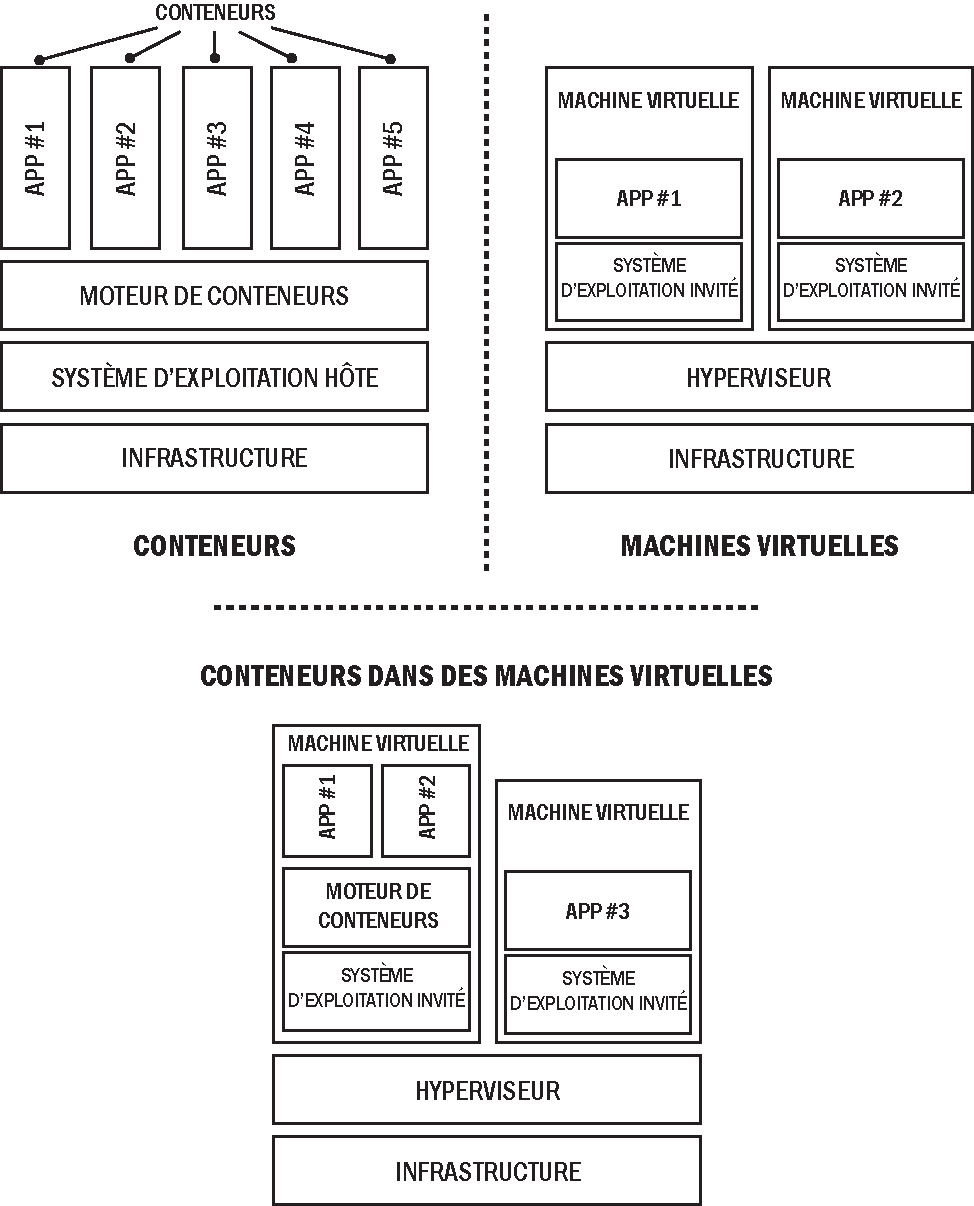
\includegraphics[width=.8\linewidth]{chapter5/containers_vms.pdf}
		\caption{Les trois principales techniques de virtualisation pour la mise en place d'une architecture de microservices.}
	\label{fig:containers_vms}
\end{figure}

En somme, une \acs{VM} est une émulation d'un système informatique tandis que les conteneurs sont toutes les unités logicielles qui regroupent le code et toutes ses dépendances requises (\textit{p. ex.} les librairies ou les binaires) qui composent une application. De ce fait, celle-ci peut s'exécuter de façon fiable et rapide d'un environnement à un autre. Ces deux technologies ne sont pas incompatibles puisqu'il est possible de les utiliser ensemble. Cependant, l'exécution de conteneurs à l'intérieur de machines virtuelles est, la plupart du temps, le résultat de l'évolution d'environnements de virtualisation matures déjà existants. Généralement, les conteneurs sont exécutés directement sur le système hôte afin d'optimiser les performances et la latence ou de réduire les coûts des licences des outils de virtualisation et des systèmes d'exploitation.

\subsection{Organisation Matérielle}

L'organisation matérielle de l'implémentation de l'architecture d'habitats intelligents présentée dans ce chapitre est illustrée par la figure \ref{fig:proposed_arch}. Afin de supporter l'architecture de microservices, cette organisation repose sur un ensemble de cinq n\oe{}uds principaux (\texttt{m0}, \texttt{m1}, \texttt{m2}, \texttt{w0} et \texttt{w1}), puisque ceci représente le nombre minimum de n\oe{}uds nécessaires pour former un \textit{cluster} distribué fiable. Par ailleurs, l'implémentation proposée suggère l'utilisation de deux  n\oe{}uds supplémentaires (\texttt{f0} et \texttt{f1}) sur chacun desquels une unité de stockage de type \acs{RAID} (\acl{RAID}) est interfacée. L'objectif de ces n\oe{}uds est de fournir un système de fichiers distribué à l'ensemble du \textit{cluster}. En effet, puisque certains conteneurs ont la capacité de monter différents volumes sur le système hôte, un tel système de fichiers offre un moyen fiable de partager des données entre chaque conteneur, quel que soit le n\oe{}ud sur lequel ils s'exécutent. En outre, tous les n\oe{}uds qui composent le \textit{cluster} et le système de fichiers distribué sont connectés à un commutateur réseau pour leur permettre de communiquer entre eux. De plus, l'ensemble de l'architecture est isolé à l'intérieur d'un réseau local afin de prévenir les problèmes de sécurité qui pourraient compromettre les expériences et de préserver l'anonymat des participants. Toutefois, pour faciliter la configuration et la maintenance de l'architecture, cette dernière demeure accessible de manière \textit{ad hoc} avec un ordinateur \textit{via} un routeur qui est, quant a lui, connecté à la fois au Web et au réseau local.

\begin{figure}[H]
	\centering
	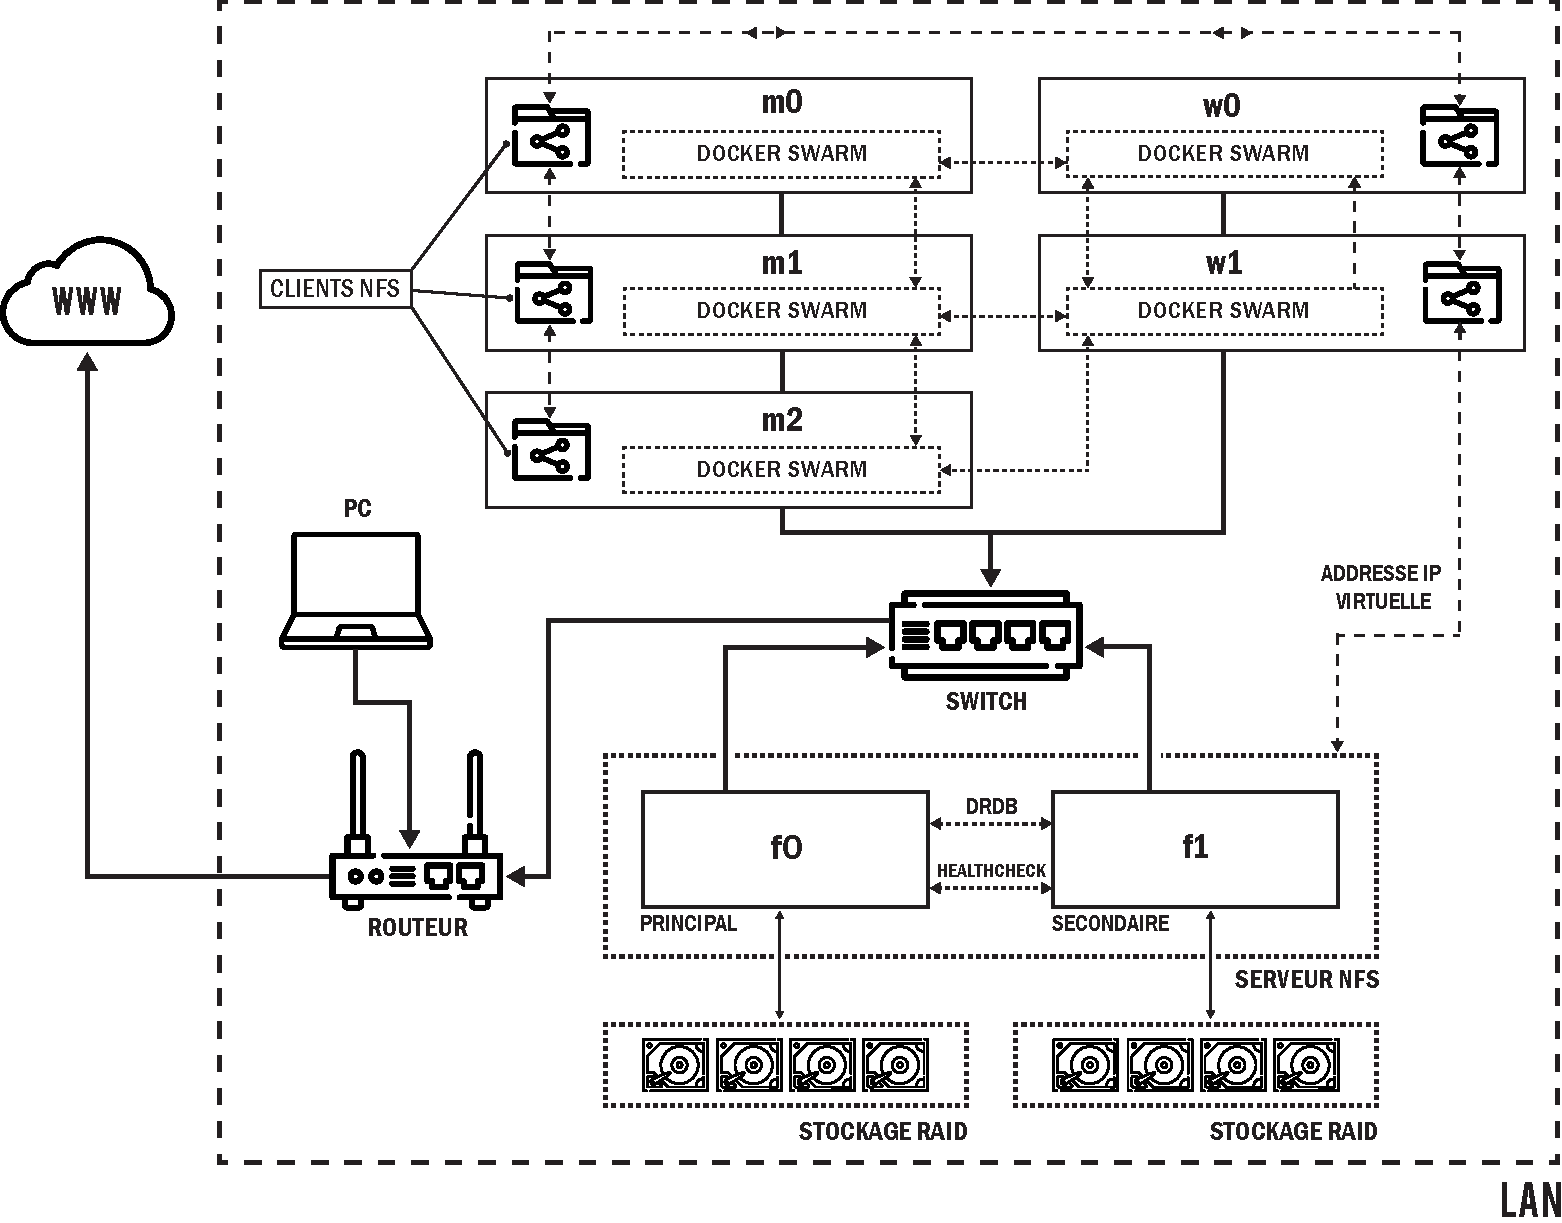
\includegraphics[width=\linewidth]{chapter5/proposed_arch.pdf}
        \caption{Organisation matérielle de l'architecture d'habitats intelligents proposée illustrant l'implémentation d'un \textit{cluster} pour le support de l'architecture de microservices ainsi que le système de fichiers distribué.}
	\label{fig:proposed_arch}
\end{figure}

\subsection{Système de fichiers distribué}

Le système de fichiers distribué fourni par les n\oe{}uds \texttt{f0} et \texttt{f1} repose sur le protocole \ac{NFS}. Le principe de ce protocole reste simple, car il est implémenté selon le modèle client/serveur. Un serveur \acs{NFS} gère l'authentification, l'autorisation, l'administration des clients ainsi que les données. Ainsi, une fois autorisés, les clients NFS peuvent accéder aux données distantes de la même manière qu'ils le font localement. En ce sens, chaque n\oe{}ud qui compose le \textit{cluster} est autorisé à accéder (lecture) et à manipuler les fichiers (création, mise à jour, suppression) de manière classique. Néanmoins, tous les autres n\oe{}uds seront informés des changements qui en résultent.

Cependant, puisque l'idée est de proposer une architecture fiable, le fait de n'avoir qu'un seul serveur \acs{NFS} ne satisfaisait pas cette contrainte. En ce sens, l'outil \acs{DRDB}\footnote{\url{https://www.linbit.com/drbd/}} (\acl{DRDB}) a été mis en place afin que les n\oe{}uds \texttt{f0} et \texttt{f1} puissent proposer un système de fichiers à la fois distribué, mais aussi répliqué. \acs{DRDB} a été paramétré pour effectuer une réplication complète des données stockées entre le serveur principal (\texttt{f0}) et le serveur secondaire (\texttt{f1}), soit le même fonctionnement qu'un système de stockage de type \acs{RAID} 1 en réseau. Afin de favoriser l'intégrité des données plutôt que la vitesse de réplication, la mise en place d'une réplication synchrone constante entre le n\oe{}ud principal et le n\oe{}ud secondaire a été adoptée plutôt qu'une réplication asynchrone ou semi-synchrone. Ainsi, les opérations de manipulation des fichiers réalisées sur le n\oe{}ud principal ne sont considérées comme terminées que lorsque les écritures sur le disque local et sur le disque distant du n\oe{}ud secondaire sont confirmées par ce dernier. Néanmoins, \acs{DRDB} ne fournit aucune fonctionnalité relative à un quelconque mécanisme garantissant la fiabilité du système de fichiers en cas de panne d'un des deux n\oe{}uds. En ce sens, l'outil Heartbeat\footnote{\url{http://www.linux-ha.org/doc/man-pages/re-heartbeat.html}} a également été adopté dans cette implémentation. Cet outil permet de proposer un mécanisme permettant de garantir la haute disponibilité du système de fichiers distribué. En tant que processus d'arrière-plan, le logiciel vise à surveiller l'état des deux serveurs \acs{DRDB}. En cas de défaillance du n\oe{}ud principal (\texttt{f0}), l'adresse \ac{VIP} du système de fichiers distribué qui pointe vers \texttt{f0} est automatiquement réaffectée pour identifier le n\oe{}ud secondaire (\texttt{f1}). Ainsi, l'accès aux données n'est en aucun cas compromis lors de la perte d'un seul n\oe{}ud, puisque cette opération est effectuée de manière transparente pour les clients \acs{NFS}.

\subsection{Orchestration des conteneurs}

L'implémentation de l'architecture de microservices proposée dans ce chapitre repose d'abord sur le moteur de conteneurs Docker\footnote{\url{https://www.docker.com}}, qui a été installé sur chaque n\oe{}ud qui compose le \textit{cluster} (\texttt{m0}, \texttt{m1}, \texttt{m2}, \texttt{w0} et \texttt{w1}). De plus, afin de pouvoir mettre en place le \textit{cluster} distribué grâce à l'ensemble de ces n\oe{}uds, il était nécessaire d'utiliser un orchestrateur. L'orchestration de conteneurs fait référence à un ensemble de techniques qui permettent de gérer les différents cycles de vie des conteneurs ainsi que leurs environnements dynamiques. Plus précisément, les outils d'orchestration permettent d'automatiser plusieurs tâches telles que la configuration, l'ordonnancement, l'approvisionnement et le passage à l'échelle des conteneurs, mais également la répartition de charge, l'allocation des ressources et la sécurité des interactions entre les conteneurs. Il existe actuellement plusieurs outils d'orchestration de conteneurs populaires tels que Kubernetes\footnote{\url{https://kubernetes.io}}, Apache Mesos\footnote{\url{https://mesos.apache.org}} et Docker Swarm\footnote{\url{https://docs.docker.com/engine/swarm/}}. Pour notre architecture, c'est l'outil Docker Swarm qui a été adopté. Plusieurs facteurs ont motivé ce choix. Tout d'abord, cet outil est plus simple à mettre en place puisqu'il est conditionné, distribué et totalement intégré au moteur de conteneur qui est déjà utilisé. En outre, bien qu'il est considéré comme moins extensible parmi les trois outils mentionnés, celui-ci offre, tel que détaillé dans la suite de cette section, tous les mécanismes requis pour créer et gérer le \textit{cluster} de cette architecture.

De manière générale, un \textit{cluster} Docker Swarm est composé de plusieurs n\oe{}uds sur lesquels le moteur Docker est installé. Ces n\oe{}uds peuvent adopter deux types de rôles\textemdash un rôle de gestionnaire (\textit{manager}) ou un rôle de travailleur (\textit{worker}). Les n\oe{}uds de type \textit{manager} sont ceux qui reçoivent les fichiers de définition des services à exécuter au sein du \textit{cluster}. De plus, les \textit{managers} distribuent les tâches qui composent ces services aux n\oe{}uds de type \textit{worker}, en fonction de leurs fichiers de définition. Ainsi, ce sont les n\oe{}uds \textit{manager} qui sont responsables de l'orchestration et de la gestion du \textit{cluster}. Dans ce contexte, les services font référence à un ensemble de tâches, c'est-à-dire des conteneurs, qui doivent s'exécuter sur les n\oe{}uds travailleurs du \textit{cluster} pour réaliser un processus donné. Néanmoins, il est tout à fait possible de définir une politique de placement manuellement. Ainsi, un service peut être soit global, soit répliqué. Lorsqu'un service est global, une unique instance est déployée sur chaque n\oe{}ud du \textit{cluster} qui est disponible, et ce, sans tenir compte de son rôle.  À l'inverse, lorsqu'un service est répliqué, il est nécessaire de préciser, dans le fichier de définition, le nombre de répliques qui doivent être déployées ainsi que le type de n\oe{}uds sur lesquelles elles seront exécutées. Un des n\oe{}uds \textit{manager} est alors en charge d'établir cette répartition. Par ailleurs, afin que les n\oe{}uds \textit{manager} puissent suivre l'évolution de l'exécution des services, les n\oe{}uds travailleurs incluent un agent dont le rôle est de rendre compte, aux \textit{managers}, de l'état des services qui lui sont attribués. Par défaut, les n\oe{}uds \textit{manager} sont également des n\oe{}uds travailleurs, mais il est possible de les configurer de manière à ce qu'ils n'acceptent aucune charge de travail en plus de leurs tâches de gestion du \textit{cluster}.

En ce qui concerne les \textit{managers}, puisqu'ils représentent les n\oe{}uds les plus importants pour la stabilité du \textit{cluster}, il est nécessaire que ce dernier en comporte plusieurs. Plus précisément, préférablement un nombre impair, selon les recommandations préconisées par Docker Swarm. En effet, parmi tous les n\oe{}uds de type \textit{manager}, l'un d'entre eux est élu en tant que leader par tous les autres \textit{managers} selon une implémentation de l'algorithme de consensus Raft \citep{MacKenzie2006}. Ainsi, ce n\oe{}ud particulier est responsable de toutes les décisions pour l'ensemble du groupe de \textit{managers}. Bien qu'il n'y ait pas de limite quant au nombre de n\oe{}uds gestionnaires que peut admettre un \textit{cluster} Docker Swarm, la décision concernant l'effectif à mettre en place reste un compromis entre la performance et la tolérance aux pannes. En effet, si le n\oe{}ud élu comme leader du \textit{cluster} devient indisponible, n'importe quel autre \textit{manager} peut obtenir ce rôle si le quorum Raft, c'est-à-dire, un accord majoritaire entre les n\oe{}uds gestionnaires, est possible. Plus précisément, l'algorithme Raft tolère jusqu'à $\lfloor(N-1)/2\rfloor$ défaillances et exige un quorum de $\lfloor(N/2) + 1\rfloor$ membres pour permettre une décision, où $N$ fait référence au nombre de n\oe{}uds \textit{manager}. Il apparaît donc clairement qu'un tel processus peut créer une surcharge du trafic réseau avec un nombre élevé de \textit{managers}, impactant alors la performance globale du \textit{cluster}. En ce sens, nous avons opté pour un \textit{cluster} de cinq n\oe{}uds, soit trois gestionnaires et deux travailleurs, ceci dans le but de tolérer une défaillance complète d'un n\oe{}ud, quel que soit son rôle. De plus, un tel nombre de \textit{managers} permet de respecter la contrainte d'avoir un nombre impair de n\oe{}uds gestionnaires pour que le quorum demeure toujours valide en cas de panne.

Pour permettre aux conteneurs de communiquer entre eux au sein du \textit{cluster} Docker Swarm, un pilote réseau spécifique a été utilisé. Ce pilote permet de créer des réseaux superposés (\textit{overlay networks}) en s'appuyant sur la technologie de tunnelisation \ac{VXLAN} \citep{rfc7348} qui permet l'encapsulation de trames réseau de la couche 2 dans \acs{UDP} (couche 4). Ainsi, dans un contexte de virtualisation comme celui imposé par les conteneurs, ce pilote permet de simplifier la complexité de la gestion des différents réseaux virtuels nécessaires à la communication entre les conteneurs qui sont déployés de manière éparse sur les différents n\oe{}uds du \textit{cluster}. De plus, les réseaux superposés offrent des mécanismes qui permettent de s'assurer du bon fonctionnement de la redondance d'un point de vue réseau au sein du \textit{cluster}. Lorsqu'un \textit{cluster} Docker Swarm est initialisé, un réseau \textit{ingress} est automatiquement créé sur chaque n\oe{}ud. Il s'agit d'un réseau superposé particulier dont l'objectif est de faciliter la répartition de la charge des différents services entre les n\oe{}uds du \textit{cluster}. Il est ensuite possible de créer autant de réseaux superposés que nécessaire pour interconnecter les conteneurs qui ont besoin d'échanger des données.

Par ailleurs, un réseau de type pont (\textit{bridge network}) est également créé automatiquement sur chaque n\oe{}ud lors de l'initialisation du \textit{cluster}. Ces réseaux sont nécessaires pour relier tous les réseaux superposés (y compris le réseau \textit{ingress}) au réseau physique des n\oe{}uds du \textit{cluster}. Par conséquent, comme les réseaux de type pont se situent au-dessus de la couche réseau du système hôte, une communication entre les conteneurs interconnectés par un réseau superposé, mais s'exécutant dans des n\oe{}uds différents, est rendue possible. Par défaut, ces communications sont chiffrées à l'aide de l'algorithme AES-GCM \citep{rfc5288}. Les n\oe{}uds \textit{manager} du cluster assurent le remplacement de la clé de chiffrement qu'ils partagent toutes les douze heures, ceci dans le but d'assurer un niveau de sécurité acceptable sans pour autant compromettre les performances des communications réseau.

Puisque les réseaux superposés attribuent dynamiquement une adresse \acl{VIP} à chaque conteneur lors de leur création, ceux-ci sont isolés d'un point de vue du réseau, ce qui simplifie donc la consommation des services. Toutefois, lorsque le nombre de services devient important, il peut sembler pertinent de connaître à l'avance certaines \acsp{VIP}, ce qui n'est évidemment pas possible. Pour résoudre ce problème, l'orchestrateur Swarm propose un mécanisme de découverte de services. Cette fonctionnalité repose sur un serveur DNS qui est intégré dans le moteur de conteneur de chaque n\oe{}ud. Ce dernier est alors chargé de résoudre le nom des services pour permettre le routage des requêtes réseau vers les conteneurs correspondants grâce à leurs \acsp{VIP} associées. En d'autres termes, le nom d'un service donné peut, par exemple, être utilisé en remplacement de son adresse \acl{VIP} dans un fichier de configuration. Ainsi, cette référence est interprétée correctement grâce au processus de découverte de services dès lors que la \acs{VIP} est fixée.

Néanmoins, lorsque les services sont répliqués, le mécanisme de découverte de services seul n'est plus suffisant. En ce sens, grâce à l'orchestrateur,  un mécanisme de répartition est mis en place dans le but de déterminer quelle réplique d'un service en particulier est utilisée. Ainsi, Docker Swarm s'appuie sur le protocole \ac{IPVS}, une implémentation de la répartition de charge qui est déjà intégrée au niveau de la couche réseau transport du noyau Linux. Grâce à ce protocole, les requêtes \acs{TCP}/\acs{UDP} inter-services peuvent donc être redirigées correctement vers les conteneurs appropriés. Dans le cas spécifique d'un \textit{cluster} Docker Swarm, chaque n\oe{}ud écoute sur les ports qui sont exposés par les services qui doivent être accessibles à distance depuis un environnement extérieur (\textit{p. ex.} un tableau de bord web qui écoute sur le port \texttt{8080}). Ensuite, \acs{IPVS} applique une répartition de la charge selon l'algorithme Round-Robin \citep{Ghaffarinejad2014} pour transmettre la demande à l'une des instances actives du service en question. Comme le montre la figure \ref{fig:swarm_load_balancing}, si le n\oe{}ud sollicité ne contient aucune réplique du service demandé par un client, alors \acs{IPVS} va router la requête à une réplique active présente sur un autre n\oe{}ud, ce qui est possible grâce au réseau superposé de type \textit{ingress}.

\begin{figure}[H]
	\centering
	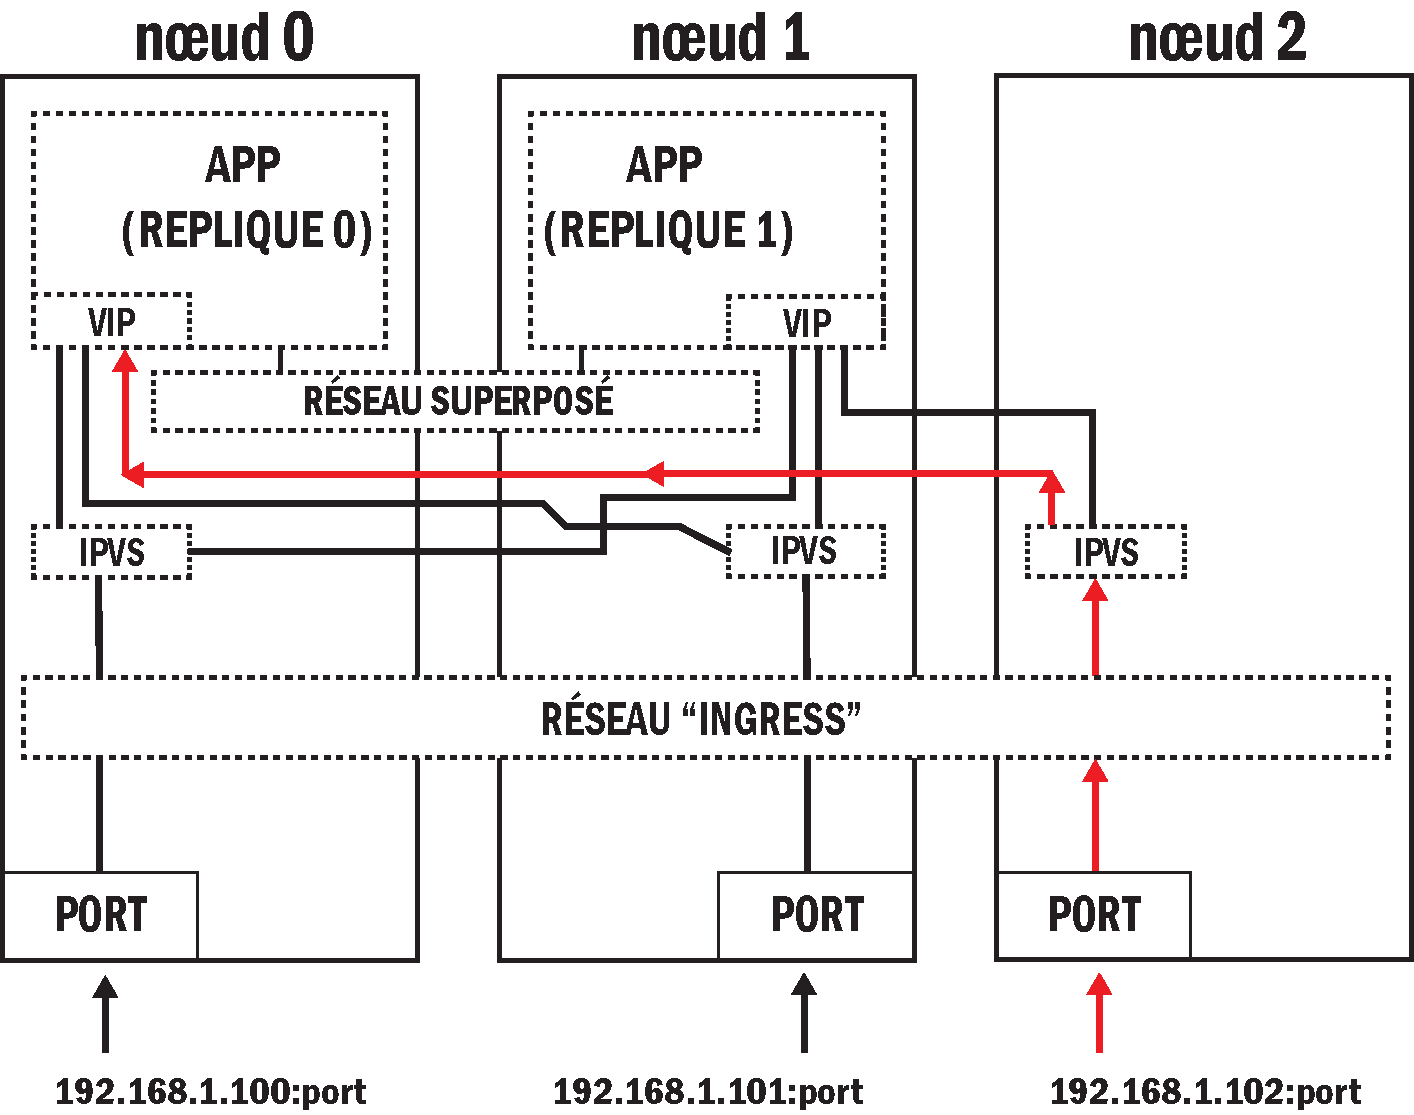
\includegraphics[width=.8\linewidth]{chapter5/swarm_load_balancing.pdf}
        \caption{Exemple du fonctionnement de la répartition de la charge selon l'algorithme Round-Robin appliquée par le protocole \acs{IPVS} sur lequel repose Docker Swarm où un des itinéraires possibles pour une requête faite sur le service répliqué \texttt{App} est identifié par des flèches rouges.}
	\label{fig:swarm_load_balancing}
\end{figure}

\subsection{Proxy inverse}

Puisque notre architecture est composée d'un \textit{cluster} de cinq n\oe{}uds, tous les services qui y sont déployés demeurent accessibles \textit{via} cinq points d'entrée différents, étant donné que l'orchestrateur ouvre tous les ports de ces services sur chacun des n\oe{}uds du \textit{cluster}. Cependant, avec un nombre important de services, il peut s'avérer difficile de gérer quel service est publié sur quel port. Ainsi, puisque la répartition de la charge au niveau des services est réalisée \textit{via} l'orchestrateur, il semble indispensable de proposer une répartition de la charge au niveau des n\oe{}uds également. Ceci dans le but de proposer un accès externe unifié et sécurisé aux services internes par le biais d'une \acs{URL} (\acl{URL}) telle que \texttt{https://service.domain.com}. Pour ce faire, l'outil open-source Tr\ae{}fik\footnote{\url{https://traefik.io}} a été préféré à d'autres options telles que NGINX\footnote{\url{https://www.nginx.com}} ou HAProxy\footnote{\url{https://www.haproxy.org}}, car il est le mieux adapté aux architectures basées sur des microservices. En effet, le principal avantage de Tr\ae{}fik est sa capacité à découvrir automatiquement les informations réseau et les services disponibles dans le \textit{cluster} et à mettre à jour dynamiquement sa configuration en fonction de l'évolution de l'environnement. Ces fonctionnalités sont particulièrement importantes avec l'utilisation de  microservices, car ceux-ci sont généralement sans état (\textit{stateless}), mais aussi car leur durée de vie est souvent courte et de nouvelles versions peuvent avoir à être déployées fréquemment. De plus, leurs instances peuvent être mises à l'échelle de façon dynamique en fonction de l'augmentation de la demande.

Tr\ae{}fik est considéré comme un proxy inverse, c'est-à-dire le principal point d'entrée d'un réseau privé. En effet, les proxys inverses sont, la plupart du temps, placé derrière un pare-feu et leur rôle est d'acheminer les requêtes entrantes des clients vers un des n\oe{}uds du \textit{cluster} et le service correspondant. En outre, les proxys inverses peuvent également remplir un certain nombre d'autres fonctions importantes pour améliorer l'efficacité et la sécurité des systèmes sur lesquels ils sont mis en place. Tout d'abord, en ce qui concerne Tr\ae{}fik, ce dernier fournit une répartition de la charge au niveau des n\oe{}uds ce qui permet de répartir les requêtes à l'ensemble des n\oe{}uds actifs au sein du \textit{cluster} pour éviter que l'un d'entre eux ne soit saturé. De plus, cet outil permet également de masquer l'organisation interne de l'architecture, car il apporte une couche supplémentaire de protection en ne dévoilant jamais l'adresse IP du n\oe{}ud qui traite réellement les requêtes. Enfin, toujours dans une optique d'offrir une meilleure protection, les proxys inverses, et plus particulièrement Tr\ae{}fik, permettent de chiffrer les échanges de données entre les clients et les services de l'architecture grâce à un ou plusieurs certificats \acs{TLS} associés aux différents services ou sous-domaines. La figure \ref{fig:arch_reverse_proxy} illustre un exemple de ce fonctionnement. En effet, Tr\ae{}fik propose un point d'entrée unique qui permet d'accéder au service \texttt{App} \textit{via} une \acs{URL} sécurisée : \texttt{https://liara.uqac.ca/app}. Ainsi lorsque cette requête est soumise par le client (\textit{p. ex. } un navigateur web), le répartiteur interne de Tr\ae{}fik achemine la requête vers l'une des répliques actives du service \texttt{App}. Dans ce scénario, la répartition de la charge fournie par l'orchestrateur Docker Swarm n'est pas représentée pour simplifier la figure, mais celle-ci demeure tout de même active et opérationnelle. En effet, bien que Tr\ae{}fik ait routé la requête vers le \texttt{n\oe{}ud 1}, il est possible que le répartiteur de charge du \textit{cluster}, quant à lui, achemine en interne la demande vers la \texttt{réplique 0} du service \texttt{App} qui s'exécute sur le \texttt{n\oe{}ud 0}.

\begin{figure}[H]
	\centering
	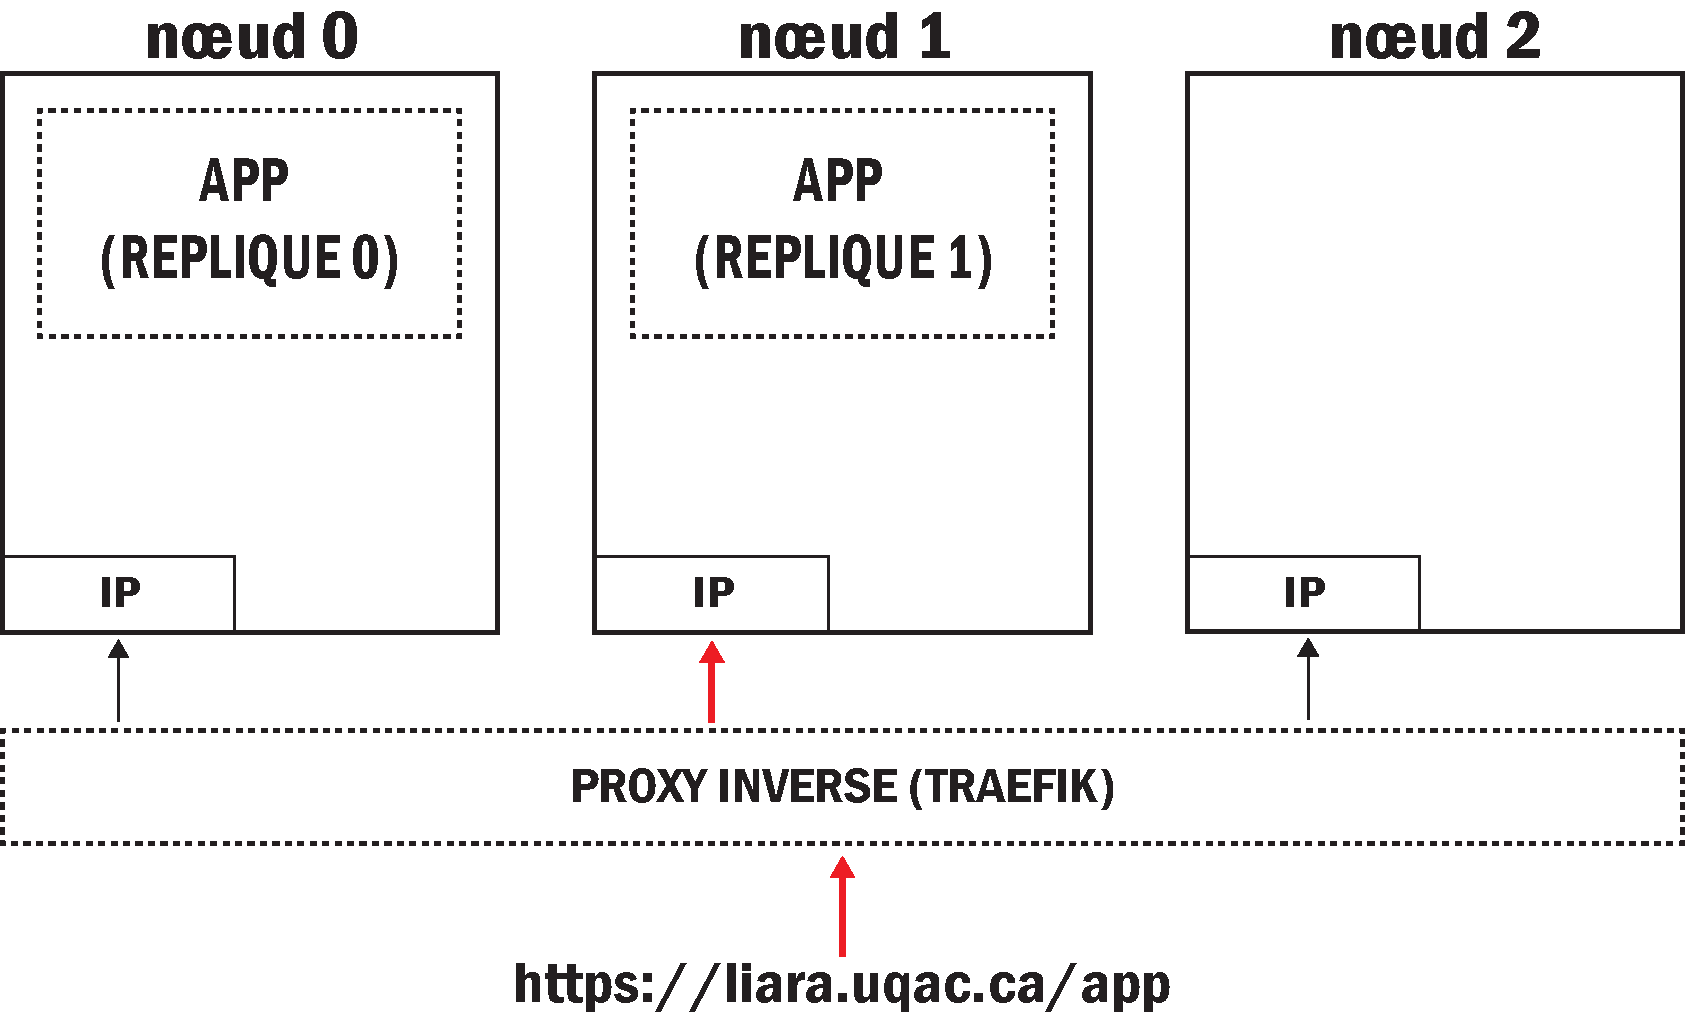
\includegraphics[width=.8\linewidth]{chapter5/arch_reverse_proxy.pdf}
        \caption{Exemple du fonctionnement du proxy inverse Tr\ae{}fik lorsqu'une requête pour accéder au service \texttt{App} est effectuée par un client \textit{via} une \acs{URL} sécurisée.}
	\label{fig:arch_reverse_proxy}
\end{figure}

\subsection{Gestion du \textit{cluster}}

Le moteur de conteneurs Docker incluant l'orchestrateur Docker Swarm est un outil qui est utilisé à travers une interface en ligne de commandes \acs{CLI}. Ainsi, il demeure possible d'initialiser et de gérer le \textit{cluster} Docker Swarm qui régit notre architecture selon plusieurs méthodes. La plupart du temps, la méthode d'initialisation la plus appropriée consiste en l'utilisation d'un outil de gestion de configuration tel qu'Ansible\footnote{\url{https://www.ansible.com}} qui permet d'automatiser les tâches d'administration de systèmes. Cependant, comme notre architecture admet une taille raisonnable et demeure relativement simple, nous avons choisi d'initialiser le \textit{cluster} manuellement grâce à divers scripts shell et fichiers de configuration. En effet, alors que les outils d'automatisation offrent une meilleure gestion des flux opérationnels d'administration de systèmes complexes ainsi qu'une meilleure flexibilité globale, les scripts shell nous ont semblé être le meilleur compromis à adopter étant donné le contexte encore expérimental de cette architecture.

Par ailleurs, la gestion du \textit{cluster} au quotidien \textit{via} une interface en ligne de commandes a été jugée trop contraignante. De ce fait, le logiciel open-source Portainer\footnote{\url{https://www.portainer.io}} a été déployé comme un service à part entière au sein du \textit{cluster}. Grâce à une interface graphique (\acl{GUI} ou \acs{GUI}) conviviale et soignée montrée par la figure \ref{fig:portainer}, cet outil nous a permis de simplifier considérablement la tâche de gestion du \textit{cluster}. En effet, celle-ci a permis de réduire le risque d'erreurs induit par la complexité de certaines commandes nécessaires au pilotage du moteur de conteneurs. De plus, le choix de Portainer comme outil de gestion a également été motivé par son large éventail de fonctionnalités. Les plus importantes comprennent la gestion des images, des réseaux et des volumes de conteneurs, mais cet outil propose également une visualisation des n\oe{}uds du \textit{cluster} incluant le placement de chaque conteneur, la consultation de tous les fichiers journaux de chaque conteneur ainsi que la possibilité d'augmenter ou en diminuer le nombre de répliques pour chaque service en fonction de la charge.

\begin{figure}[H]
	\centering
	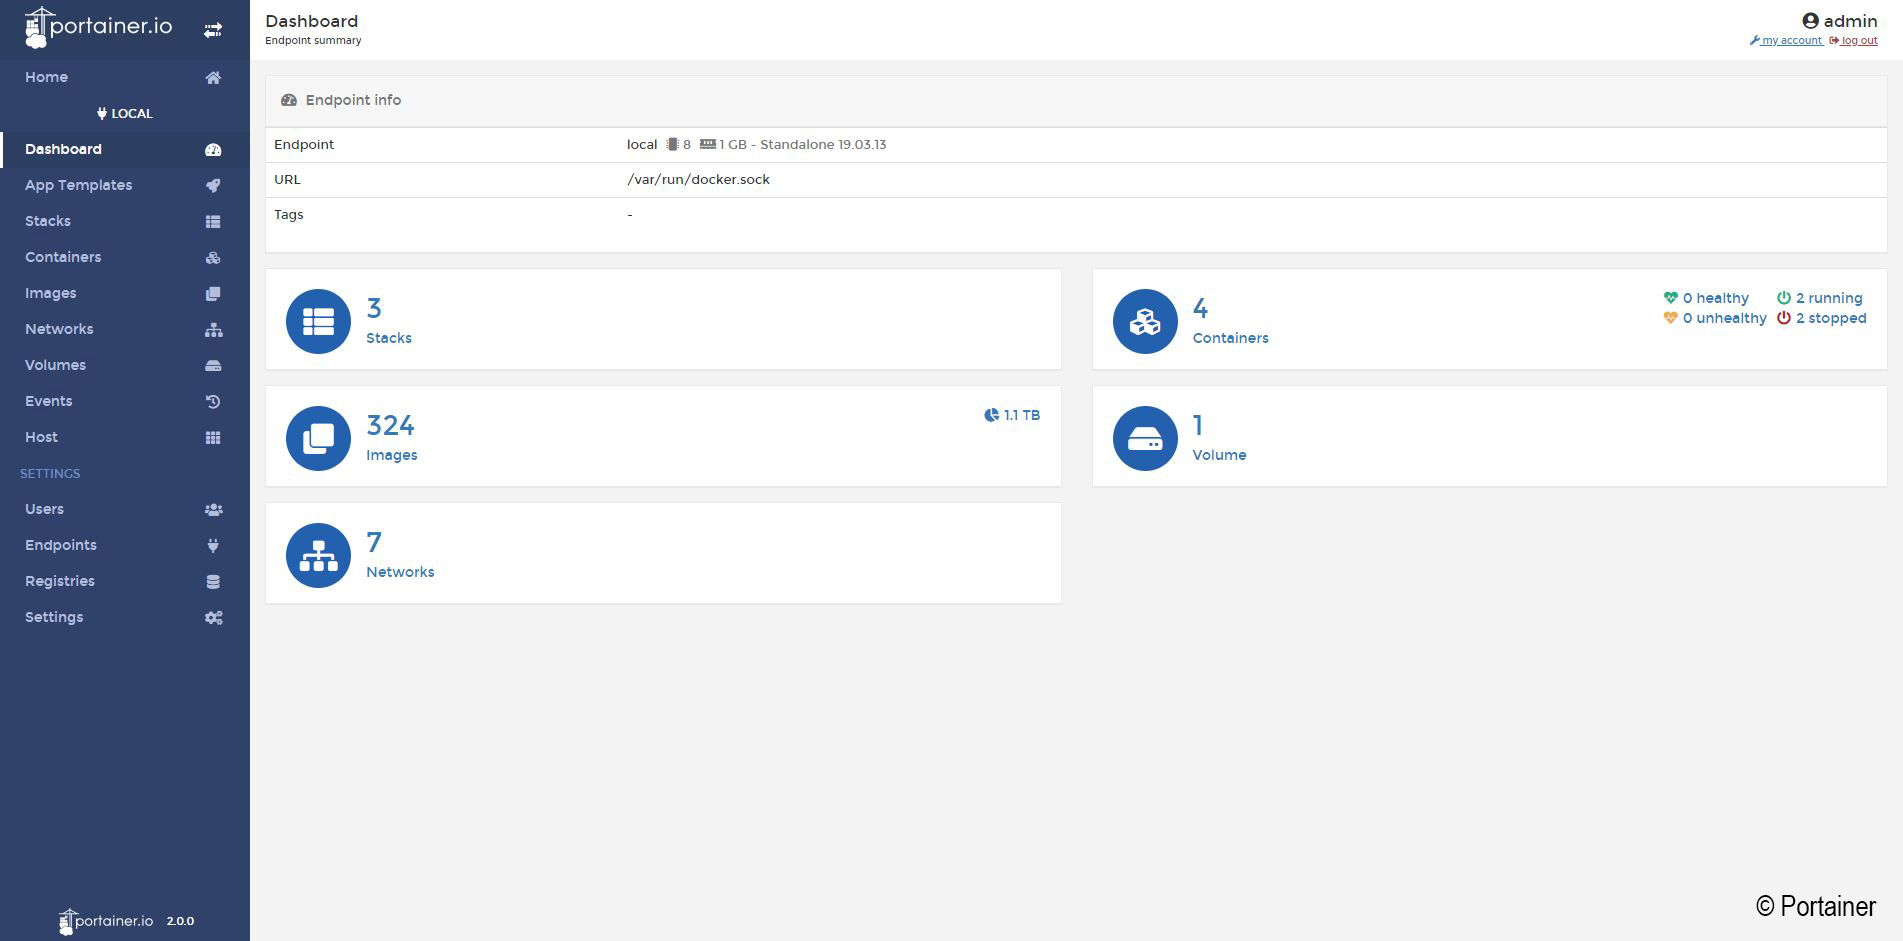
\includegraphics[width=\linewidth]{chapter5/portainer.jpg}
        \caption{Interface Graphique de l'outil Portainer déployé pour permettre la gestion du \textit{cluster}.}
	\label{fig:portainer}
\end{figure}

\subsection{Base de données répliquée}

Puisque cette architecture est conçue principalement pour les maisons intelligentes, il était important de proposer un moyen fiable de stocker les valeurs des capteurs ainsi que l'état des effecteurs. Pour ce faire, trois services ont été déployés sur le \textit{cluster}, chacun contenant une instance du \ac{SGBD} MongoDB\footnote{\url{https://www.mongodb.com}}. Ainsi, la réplication des données a été réalisée grâce à une architecture composée d'un ensemble de répliques (\textit{replica set}) à trois membres.

MongoDB est un \acs{SGBD} open-source orienté documents et non relationnel (\acs{NoSQL}), principalement utilisé pour le stockage de gros volumes de données. Un tel choix a été fait, car sa conception est axée sur la performance, la haute disponibilité et la mise à l'échelle automatique. Puisqu'il s'agit d'un \acs{SGBD} orienté document, les données sont stockées dans des collections sous forme d'ensembles de documents. Ceux-ci font référence à une structure de données composée de paires de champs et de valeurs. En effet, ils sont formatés en \ac{BSON}, un format de fichier similaire aux objets \acs{JSON} où les champs peuvent également inclure d'autres documents, des tableaux et des ensembles de documents. Ce type de modèle de base de données dit semi-structuré implique qu'il n'existe pas de séparation entre les données et le schéma qui les représente. Ainsi, le principal avantage de l'approche orientée documents reste d'abord la possibilité de représenter des relations hiérarchiques complexes avec un seul enregistrement. Aussi, de tels modèles de données facilitent la répartition des données entre plusieurs n\oe{}uds de base de données, ce qui simplifie le processus de mise à l'échelle.

Dans le contexte de MongoDB, un ensemble de répliques constitue un groupe d'instances de base de données qui maintiennent le même ensemble de données en fournissant de la redondance ainsi qu'une haute disponibilité pour garantir la tolérance aux pannes. Le déploiement d'un tel ensemble peut se faire principalement selon deux types d'architectures différentes. Dans un premier cas, l'architecture est composée au minimum d'un n\oe{}ud principal et de deux n\oe{}uds secondaires. Le second type d'architecture, quant à lui, reprend les mêmes caractéristiques du premier type, mais doit également admettre un n\oe{}ud arbitre. Un n\oe{}ud principal est le seul membre d'un ensemble qui tolère les opérations d'écriture. Les n\oe{}uds secondaires sont, quant à eux, en charge de préserver une copie de l'ensemble de données du n\oe{}ud principal. Afin que le processus de réplication se déroule correctement, les n\oe{}uds secondaires appliquent les instructions du journal des opérations du n\oe{}ud principal à leur propre ensemble de données, et ce, de manière asynchrone. En revanche, dans une architecture d'ensemble de répliques qui contient un arbitre, ce dernier ne dispose pas de copie de l'ensemble de données du n\oe{}ud principal. Ainsi, le n\oe{}ud arbitre ne peut, d'aucune façon, devenir un n\oe{}ud principal en cas de panne de ce dernier. Toutefois, le n\oe{}ud arbitre participe à l'élection d'un nouveau n\oe{}ud principal lorsque cela est nécessaire. En ce sens, dans le cas d'un ensemble de répliques à trois membres, la mise en \oe{}uvre d'une architecture composée d'un n\oe{}ud principal et de deux n\oe{}uds secondaires a été préférée. En effet, le fait de remplacer un n\oe{}ud secondaire par un arbitre ne permet pas de garantir une aussi bonne répartition de la charge lors des opérations de lecture des données.

La figure \ref{fig:mongodb_replication} illustre le fonctionnement de cette architecture d'ensemble de répliques composée d'un n\oe{}ud principal et de deux n\oe{}uds secondaires (P-S-S). Toutes les deux secondes, tous les n\oe{}uds s'envoient des pouls (\texttt{A}); dans le cas où l'un d'entre eux ne revient pas à son émetteur dans les dix secondes, les n\oe{}uds restants identifient alors le n\oe{}ud non réactif comme inaccessible (\texttt{B}). Lorsque c'est le n\oe{}ud principal qui est indisponible, un processus d'élection est alors déclenché pour que l'un des deux n\oe{}uds secondaires devienne le nouveau n\oe{}ud principal (\texttt{C}). De la même manière que pour l'orchestration du \textit{cluster}, la recommandation qui est formulée dans la documentation pour déployer un ensemble de répliques MongoDB est de mettre en place un nombre total de n\oe{}uds impair. Ainsi, il est possible, dans le cas d'une architecture P-S-S comme celle-ci, de subir la perte totale d'une instance de la base de données. En effet, les quorums de tolérance aux pannes demeurent identiques pour les deux composants logiciels.

\begin{figure}[H]
	\centering
	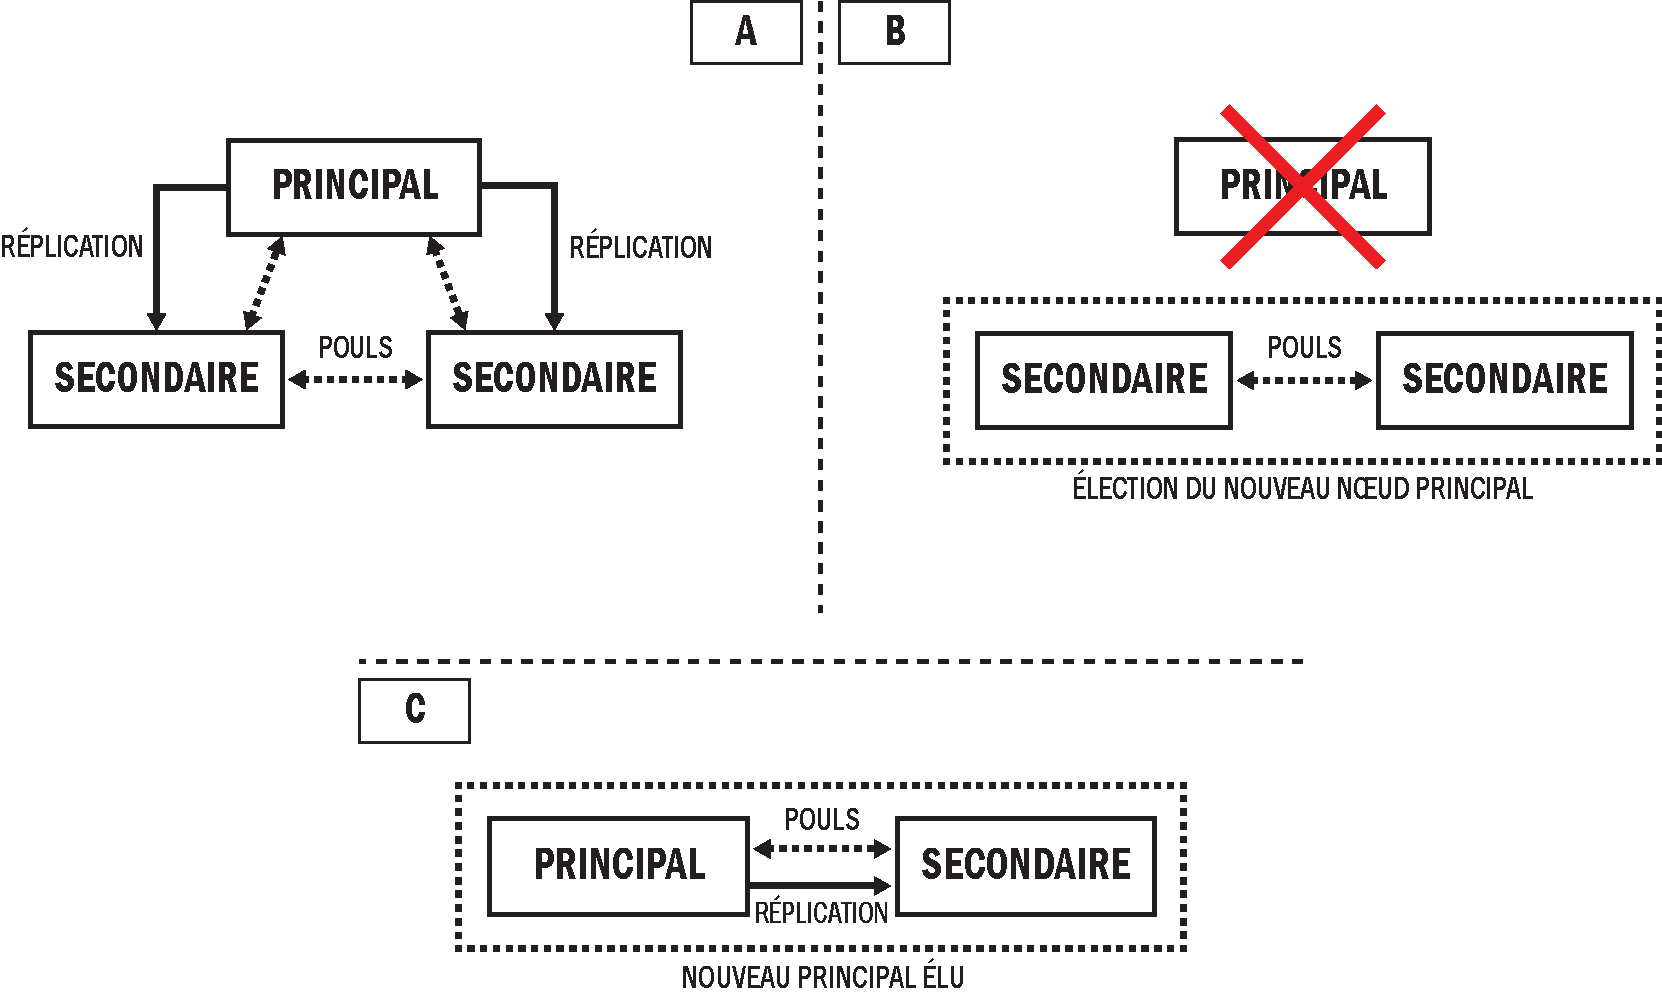
\includegraphics[width=.9\linewidth]{chapter5/mongodb_replication.pdf}
        \caption{Processus d'élection avec la base de données MongoDB selon l'architecture d'ensemble de répliques à trois n\oe{}uds de type P-S-S où \texttt{A}, \texttt{B} et \texttt{C} représentent respectivement les étapes successives lors de la perte totale du n\oe{}ud principal.}
	\label{fig:mongodb_replication}
\end{figure}

\subsection{Dépôt d'images de conteneurs}

Le principal avantage de l'utilisation d'une architecture de microservices, en particulier dans un environnement comme celui des laboratoires de recherche dans le domaine des habitats intelligents, est de fournir un moyen simple de déployer des composants logiciels expérimentaux qui fonctionnent dans des conteneurs pour réaliser la reconnaissance d'activités. Ainsi, dans le but de faciliter la gestion de versions (\textit{versionning}), la distribution et la réutilisation de ces composants, un système de stockage des images des conteneurs a été mis en place au sein du \textit{cluster}.

Les images sont des fichiers immuables qui sont composés de plusieurs couches contenant le code source, les librairies, les dépendances ainsi que les outils nécessaires au bon fonctionnement des conteneurs. En d'autres termes, les images décrivent les services et leur environnements virtuels à un instant donné. Finalement, les conteneurs ne représentent que des images qui sont en cours d'exécution. En ce sens, celles-ci peuvent être stockées dans un dépôt, où les répertoires qu'il admet contiennent les différentes versions pour chacune des images. Grâce à un tel registre, il devient possible pour les expérimentateurs de télécharger certaines images (\textit{pull}), d'en créer (\textit{push}) de nouvelles contenant leurs propres composants logiciels ou de créer de nouvelles versions d'images déjà existantes. Par défaut, le moteur de conteneurs installé sur chaque n\oe{}ud de l'architecture est configuré pour utiliser le dépôt public DockerHub\footnote{\url{https://hub.docker.com}}. Cependant, puisque les applications expérimentales conçues dans les environnements de recherche peuvent contenir des vulnérabilités, des informations confidentielles ou un certain nombre d'innovations, la configuration du moteur de conteneurs a été modifiée afin que ce dépôt privé d'images puisse être utilisé dans le \textit{cluster}.

\subsection{Organisation des conteneurs}
\label{sec:cont_org}

Pour résumer les différents aspects qui décrivent la conception de l'architecture proposée et qui ont été introduits dans ce chapitre, la figure \ref{fig:containers} propose une représentation graphique du déploiement des conteneurs sur les n\oe{}uds qui composent le cluster. De plus, les réseaux superposés pour chaque service y sont également illustrés.

\begin{figure}[H]
	\centering
	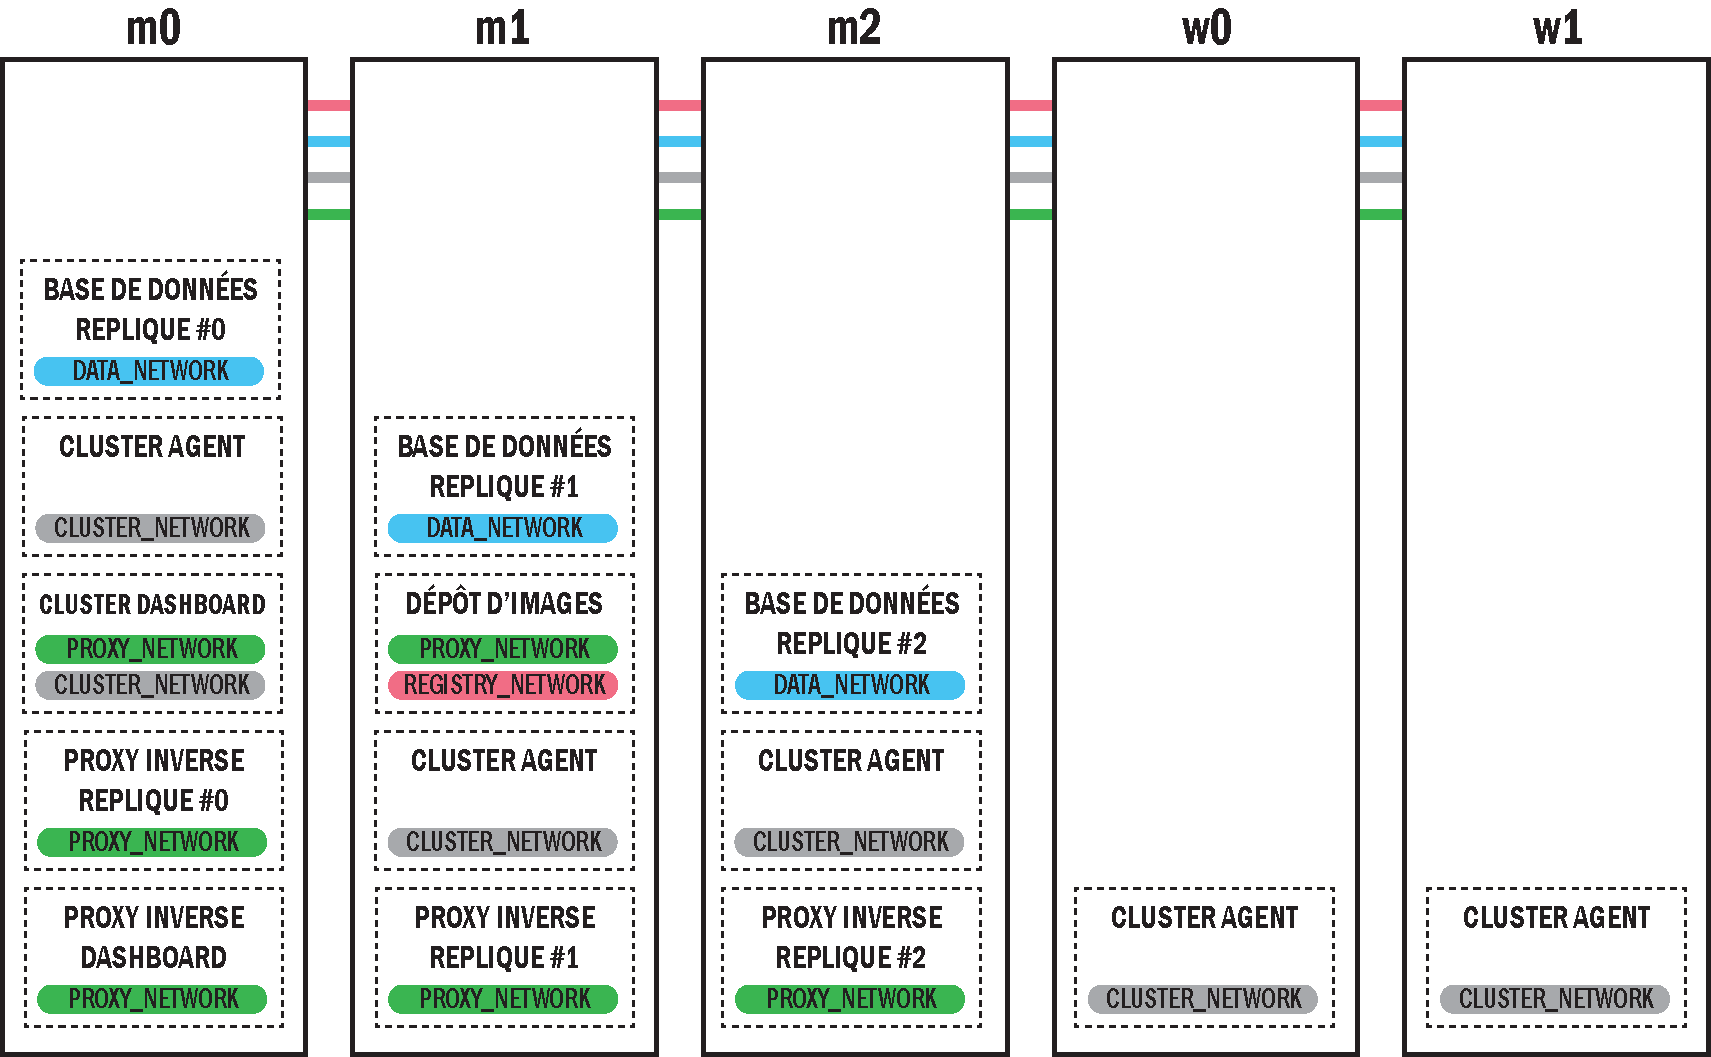
\includegraphics[width=.9\linewidth]{chapter5/containers.pdf}
        \caption{Déploiement des conteneurs sur les n\oe{}uds du \textit{cluster} qui décrivent la conception de l'architecture proposée.}
	\label{fig:containers}
\end{figure}

Dans ce déploiement, il est possible de voir que l'application Tr\ae{}fik admet deux services distincts. Le premier concerne le service de proxy inverse dont trois répliques sont exécutées sur chacun des n\oe{}uds de gestion du \textit{cluster} (\texttt{m0}, \texttt{m1}, \texttt{m2}). Ce placement a été privilégié, car cela permet de s'assurer de la fiabilité d'un élément aussi important en cas de perte d'un \textit{manager}. Le second service est, quant à lui, le tableau de bord web qui permet de visualiser, en temps réel, les routes actives vers les différents services ouverts à un environnement extérieur qui sont détectées par l'outil. De plus ce tableau de bord permet de visualiser plusieurs statistiques d'accès pertinentes pour l'évaluation de la charge en fonction des services. Néanmoins, puisque ce tableau de bord n'a pas un impact majeur sur le bon fonctionnement du cluster, son déploiement n'admet aucune réplique supplémentaire au seul conteneur qui lui est attribué. Toutefois, ce service est doté d'une politique de redémarrage qui prévoit de toujours relancer le conteneur si son exécution est interrompue. En ce sens, s'il se produit une défaillance au niveau du n\oe{}ud sur lequel il est déployé (\texttt{m0}), l'exécution du conteneur du tableau de bord de Tr\ae{}fik peut être relancée soit sur \texttt{m1}, soit sur \texttt{m2}. De la même manière, des instructions de déploiement identiques ont été définies pour le service du dépôt d'images et le service du tableau de bord de l'outil de gestion du \textit{cluster}.

Par ailleurs, en ce qui concerne la base de données, l'ensemble de répliques MongoDB a été déployé sur les n\oe{}uds de gestion dans le but de fournir, en permanence, une réplication sûre des données et de tolérer, au maximum, la défaillance d'un unique n\oe{}ud. Enfin, puisque le rôle de l'outil Portainer est de pouvoir gérer l'intégralité du \textit{cluster}, un agent, c'est-à-dire, un service global a été déployé sur chaque n\oe{}ud pour permettre à l'application web de transmettre les bonnes requêtes aux différents moteurs de conteneurs présents sur chacun des n\oe{}uds.

En ce qui concerne la communication réseau, un réseau superposé a été créé pour chaque service. De plus, le tableau de bord du proxy inverse est automatiquement exposé et accessible \textit{via} l'\acs{URL} suivante : \texttt{https://liara.uqac.ca/proxy}. Toutefois, puisque le tableau de bord de l'outil de gestion du \textit{cluster} et le dépôt d'images doivent également être accessibles depuis l'extérieur du \textit{cluster}, ces services sont connectés au réseau superposé du proxy inverse. Ainsi, le routage des demandes clients en ce qui concerne les accès à ces services est rendu possible \textit{via} les \acsp{URL} suivantes : \texttt{https://liara.uqac.ca/cluster} et \texttt{https://liara.uqac.ca/registry}.

\section{Experimentations}

Afin d'évaluer et de valider l'architecture introduite dans les sections précédentes, une installation expérimentale préliminaire a été déployée dans notre laboratoire, le \acs{LIARA}. En outre, plusieurs expérimentations ont été réalisées afin de confirmer la capacité pour ce système à résister à différentes défaillances qui pourraient survenir afin d'en déterminer sa fiabilité globale. Pour ce faire, cette section commence par décrire la mise en \oe{}uvre matérielle utilisée pour le fonctionnement de l'architecture. Une seconde section décrit les expérimentations qui ont été menées ainsi que les résultats qui en découlent.

\subsection{Installation Matérielle}

Afin de minimiser les difficultés dans la reproduction du déploiement de l'architecture présentée lors de ce chapitre ainsi que les expérimentations qui y ont été appliquées, la mise en \oe{}uvre de cette architecture a été faite en utilisant du matériel open-source. Pour ce faire, notre choix s'est basé sur l'utilisation de sept \acsp{SOC} Raspberry Pi 3 Model B, un routeur sans fil conventionnel (LinkSys WRT1900AC) fonctionnant avec le système d'exploitation OpenWRT\footnote{\url{https://openwrt.org}} ainsi qu'un simple commutateur réseau. Le principal avantage de l'utilisation des Raspberry Pi est qu'elles offrent un rapport qualité-prix intéressant pour les besoins de cette architecture. En effet, alors que leur coût unitaire est de 35 dollars US, celles-ci intègrent un processeur ARMv8 quadric\oe{}ur de 1,2 GHz et 1 GiB de SDRAM. De plus, pour que ce déploiement expérimental reste aussi peu onéreux que possible, le stockage n'a pas été effectué sur des systèmes RAID. Au lieu de cela, deux clés USB ont été connectées aux deux Raspberry Pi utilisées pour le système de fichiers distribué (\texttt{f0} et \texttt{f1}).

De plus, comme ce modèle en particulier de Raspberry Pi dispose d'un processeur basé sur l'architecture ARMv8, l'utilisation de systèmes d'exploitation 64-bits y est supportée. En ce sens, nous avons opté pour une version spécifique de la distribution Linux Debian\footnote{\url{https://www.debian.org}} qui a été modifiée selon nos besoins\footnote{\url{https://github.com/FlorentinTh/FlOS}}. Ce choix a été établi considérant que le système d'exploitation Raspberry Pi OS\footnote{\url{https://www.raspberrypi.org/downloads/raspberry-pi-os/}} n'est toujours pas disponible en version 64-bits malgré la sortie de nouvelles Raspberry Pi disposant de plusieurs gibibits (Gibit) de SDRAM. Puisque les conteneurs virtualisent leurs environnements au niveau du système hôte, l'emploi d'un système d'exploitation 64-bits était péremptoire. En effet, plusieurs outils qui sont requis dans la conception de notre architecture étaient disponibles uniquement pour l'architecture de processeur ARMv8 (\textit{p. ex.} MongoDB).

\subsection{Haute disponibilité}

Suivant l'initialisation du \textit{cluster} Docker Swarm sur chacun des cinq n\oe{}uds de l'architecture (\texttt{m0}, \texttt{m1}, \texttt{m2}, \texttt{w0}, \texttt{w1}), tous les composants applicatifs y ont été déployés selon la politique de placement définie en section \ref{sec:cont_org}. Ainsi, l'architecture distribuée a été opérationnelle en seulement quelques minutes. Cette politique de déploiement a été spécifiquement déterminée pour supporter la défaillance totale d'un n\oe{}ud au maximum. Cependant, bien que l'ajout de n\oe{}uds supplémentaires au \textit{cluster} doit irréfutablement améliorer la tolérance aux pannes, avoir tous ces n\oe{}uds dans le même emplacement géographique n'améliorent, en réalité, pas la fiabilité de l'ensemble du système. De plus, cela créera un environnement beaucoup plus complexe à gérer et à maintenir. Par conséquent, les différentes expérimentations réalisées sur cette architecture ont pour but de confirmer que cette implémentation demeure fiable.

Le premier protocole expérimental mis en place est relativement simple. La défaillance d'un n\oe{}ud a été simulée en débranchant son câble Ethernet au niveau du commutateur réseau afin que celui-ci ne puisse plus communiquer avec le reste du \textit{cluster}. En ce sens, nous avons commencé par déconnecter un seul n\oe{}ud de type \textit{worker} (\texttt{w0}). Cette expérimentation est identifié : \textit{\texttt{F0}}. Tel qu'attendu, tous les services déployés au sein de l'architecture sont restés accessibles et tous les conteneurs qui fonctionnaient sur \texttt{w0} ont été automatiquement répartis et relancés sur les n\oe{}uds opérationnels restants. Enfin, après avoir reconnecté ce n\oe{}ud au réseau, il a montré un état opérationnel en quelques secondes. Cependant, les conteneurs qui s'exécutaient auparavant sur \texttt{w0} n'ont pas été redémarrés sur ce n\oe{}ud d'origine, car ceux-ci étaient pleinement opérationnels sur les autres n\oe{}uds. Dans un second temps, lorsqu'un unique n\oe{}ud de gestion (\textit{manager}) a été débranché du réseau (\texttt{m2}), les mêmes résultats ont été observés (\textit{\texttt{F1}}). En revanche, lorsque le n\oe{}ud leader (\texttt{m0}) a été privé de sa connexion réseau, le processus d'élection s'est enclenché et c'est le n\oe{}ud \texttt{m2} qui a été choisi comme nouveau leader (\textit{\texttt{F2}}). Ensuite, deux n\oe{}uds de différents types ont été débranchés du commutateur réseau, soit un n\oe{}ud \textit{manager} (\texttt{m1}) ainsi qu'un \textit{worker} (\texttt{w0}), tandis que les autres sont restés connectés (\textit{\texttt{F6}}). Bien qu'avec cette architecture notre objectif était de tolérer la défaillance d'un n\oe{}ud uniquement, le bon fonctionnement du \textit{cluster} n'a pas été altéré dans cette situation. Cela peut s'expliquer par le fait que le dysfonctionnement a été simulé sur deux n\oe{}uds ayant un rôle différent. En effet, la reproduction de cette expérimentation en débranchant le câble réseau de deux n\oe{}uds gestionnaires incluant le leader (\textit{p. ex.} \texttt{m0} et \texttt{m1} ou \texttt{m0} et \texttt{m2}) a permis de constater que l'intégrité de l'ensemble de l'architecture était compromise (\textit{\texttt{F7}}). Bien que les services démarrés sur les n\oe{}uds travailleurs ont continué leur exécution normalement, la capacité, au sein du \textit{cluster}, d'effectuer des tâches de gestion, y compris le démarrage de nouveaux services était perdue. En ce sens, cette expérimentation nous permet d'affirmer qu'étant donné la mise en \oe{}uvre proposée, il demeure plus sûr de garder à l'esprit que la défaillance d'un seul n\oe{}ud reste la limite maximale à supporter, puisque selon leur type, la perte de deux n\oe{}uds peut potentiellement compromettre le bon fonctionnement du \textit{cluster}.

Dans un second temps, la procédure expérimentale précédente a été reproduite en simulant la défaillance des n\oe{}uds \textit{via} une déconnexion de leur alimentation électrique pour les arrêter, au lieu de les déconnecter du réseau (\textit{\texttt{F3}}, \textit{\texttt{F4}}, \textit{\texttt{F5}}). Bien que des résultats similaires aient été observés, le temps de récupération qui a été constaté pour chaque n\oe{}ud était plus important, c'est-à-dire, quelques minutes au lieu de quelques secondes. De plus, une expérimentation supplémentaire a été menée afin d'évaluer la résilience du \textit{cluster} en cas de coupure générale de l'alimentation électrique (\textit{\texttt{F8}}). Pour ce faire, toutes les Raspberry Pi ont été mises hors tension à l'aide du disjoncteur présent sur la multiprise à laquelle elles étaient branchées. Le routeur et le commutateur réseau, quant à eux, sont restés sous tension. Ainsi, puisque l'état du \textit{cluster} est préservé grâce à un mécanisme interne du moteur de conteneurs, le \textit{cluster} a pu restaurer son état de fonctionnement initial lui-même, après le redémarrage de chaque n\oe{}ud et le rétablissement de la communication inter-gestionnaires. Le temps total de récupération observé pour une telle coupure générale a été d'environ une dizaine de minutes. Le tableau \ref{tab:expe_recap} présente un récapitulatif de ces expérimentations ainsi que les résultats qui ont été obtenus.

\begin{table}[H]
  \centering
  \caption{Récapitulatif des expérimentations réalisées sur l'architecture afin de déterminer sa fiabilité globale.}
  \label{tab:expe_recap}
  \resizebox{\textwidth}{!}{
    \begin{tabular}{@{}rcccccc@{}}
      \toprule
        \multicolumn{1}{l}{} & \textit{\texttt{F0}}, \textit{\texttt{F3}} & \textit{\texttt{F1}}, \textit{\texttt{F4}} & \textit{\texttt{F2}}, \textit{\texttt{F5}} & \textit{\texttt{F6}} & \textit{\texttt{F7}} & \textit{\texttt{F8}} \\
      \midrule
        \textbf{N\oe{}ud(s)} & \texttt{w0} & \texttt{m2} & \texttt{m0} & \texttt{m1} \& \texttt{w0} & \texttt{m0} \& \texttt{m1} & \texttt{tous} \\
        \multirow{1}{*}{\textbf{Type de panne}} & \begin{tabular}[c]{@{}c@{}}réseau \\[-15pt] - \\[-15pt] électrique\end{tabular} & \begin{tabular}[c]{@{}c@{}}réseau \\[-15pt] - \\[-15pt] électrique\end{tabular} & \begin{tabular}[c]{@{}c@{}}réseau \\[-15pt] - \\[-15pt] électrique\end{tabular} & \begin{tabular}[c]{@{}c@{}}réseau \\[-15pt] - \\[-15pt] électrique\end{tabular} & \begin{tabular}[c]{@{}c@{}}réseau \\[-15pt] - \\[-15pt] électrique\end{tabular} & électrique \\
      \midrule
        \textbf{Tâches relancées} & oui & oui & oui & oui & non & non \\
        \textbf{Élection d'un leader} & non & non & oui & non & non & non \\
      \midrule
        \textbf{État du cluster} & disponible & disponible & disponible & disponible & H.S. & disponible \\
        \multirow{1}{*}{\textbf{Temps de récupération}}  & \begin{tabular}[c]{@{}c@{}}$\approx 1\: s$ \\[-15pt] - \\[-15pt] $\approx 1\: m$\end{tabular}  & \begin{tabular}[c]{@{}c@{}}$\approx 1\: s$ \\[-15pt] - \\[-15pt] $\approx 1\: m$\end{tabular} & \begin{tabular}[c]{@{}c@{}}$\approx 1\: s$ \\[-15pt] - \\[-15pt] $\approx 1\: m$\end{tabular} & \begin{tabular}[c]{@{}c@{}}$\approx 1\: s$ \\[-15pt] - \\[-15pt] $\approx 1\: m$\end{tabular} & - & $\approx 10\: m$ \\
      \bottomrule
    \end{tabular}
  }
\end{table}

Finalement, ces deux expériences ont prouvé que l'architecture proposée dans ce chapitre offre une fiabilité globale plus que satisfaisante. En effet, selon les situations de défaillances, elle a su démontrer sa capacité à toujours supporter la défaillance d'un n\oe{}ud. Cependant, comme les pannes électriques peuvent impliquer un temps de récupération plus long, nous suggérons que tout l'équipement nécessaire au déploiement de cette architecture soit alimenté électriquement par une source d'\ac{ASI}.

\section{Conclusion}

Dans ce chapitre, une nouvelle architecture pour les maisons intelligentes a été proposée. Par opposition aux architectures existantes, cette implémentation vise à être agnostique vis-à-vis de la conception des applications qu'elle admet, mais également fiable et évolutive. Ainsi, la conception qui a été proposée repose sur le concept de microservices mis en \oe{}uvre grâce à un \textit{cluster} composé de cinq n\oe{}uds distribués. L'utilisation de microservices permet d'améliorer à la fois l'interopérabilité entre les applications d'apprentissage machine qui constituent généralement un ensemble hétérogène de technologies, ainsi que leur réutilisabilité.

De plus, cette implémentation a été conçue pour être compatible avec la majorité des architectures de maisons intelligentes existantes, car elle peut facilement remplacer l'unité centrale de calcul (serveur ou un \textit{broker}) que celles-ci admettent. Aussi, cette architecture s'inscrit dans la continuité de l'objectif qui consiste à supprimer complètement tout point de défaillance unique au sein des habitats intelligents afin que ceux-ci puissent offrir un niveau de fiabilité plus élevé à leurs résidents.

Enfin, le dernier objectif de cette implémentation concerne la possibilité d'y ajouter des ressources supplémentaires, tant matérielles que logicielles, en fonction des besoins. Ainsi, cette architecture permet, lorsqu'elle est déployée dans un environnement de recherche, un plus grand niveau d'évolutivité, ce qui permet alors de simplifier les procédures d'expérimentations. Grâce aux évaluations qui ont été réalisées pour évaluer la haute disponibilité de cette architecture, nous avons montré que le bon fonctionnement de l'ensemble du système n'était pas affecté lors d'un dysfonctionnement complet d'un n\oe{}ud du \textit{cluster}. De plus, ces expérimentations ont également permis de révéler que l'architecture était également résistante à une panne de courant généralisée. Néanmoins, puisque le temps de récupération du \textit{cluster} après une panne électrique demeure important, il est important de suggérer l'utilisation d'une alimentation sans interruption pour prévenir ce genre de situations.

\let\cleardoublepage\clearpage
\chapter{LE2ML: un \textit{workbench} modulaire pour l'apprentissage machine}
\label{chap:6}

% Grâce aux chapitres précédents, il a été montré que les \textit{wearable devices} sont de plus en plus utilisés dans le processus de reconnaissance d'activités au sein des habitats intelligents. Aussi, ces dispositifs ont également été employés dans l'objectif de répondre à plusieurs autres problématiques relatives à l'assistance des résidents de ces habitats, au sens large. Néanmoins, l'engouement croissant pour les \textit{wearable devices} a permis d'identifier plusieurs problématiques quant à leur utilisation dans ce contexte de recherche particulier. En effet, il a été évalué que la plupart des différentes architectures d'habitats intelligents qui ont été proposées n'ont pas été conçues dans une optique évolutive. Ainsi, celles-ci ne permettent pas d'y intégrer de manière rapide et efficace de nouveaux capteurs, comme les \textit{wearable devices}, ou de nouveaux composants logiciels pour effectuer le processus de reconnaissance d'activités et l'assistance aux résidents.

% Pour ce travail, l'intégration des \textit{wearable devices} dans les architectures de maisons intelligentes s'est concentrée avant tout sur l'aspect logiciel plutôt que matériel, dans la conception des méthodes de reconnaissance que ces dispositifs proposent. En effet, tout comme pour la reconnaissance d'activités réalisée de manière classique, c'est-à-dire, en exploitant les capteurs et effecteurs ambiants présents dans l'habitat, les différents processus proposés par les dispositifs sont, dans une vaste majorité des cas, encapsulés au sein d'un unique composant logiciel immuable. De la même manière, la réutilisation de mécanismes communs, le déploiement de ces méthodes et leur modification demeurent alors des tâches complexes à mettre en \oe{}uvre.

% Malgré cela, certains travaux ont fait mention de l'emploi d'un \textit{workbench} d'apprentissage machine afin de traiter les données produites par les \textit{wearable devices} et de réaliser la reconnaissance d'activité \citep{Chapron2018}. D'un point de vue académique, ces outils ne sont pas nouveaux et ils permettent un prototypage rapide, la visualisation des données ainsi qu'une meilleure reproductibilité des méthodes expérimentales et une meilleure réutilisation des composants logiciels \citep{Holmes1994,Langlois2008}. À titre d'exemple, l'outil le plus connu et le plus répandu dans la littérature est \acs{WEKA}. Il s'agit d'un \textit{workbench} open source issue de la recherche académique qui supporte un grand nombre d'algorithmes d'apprentissage machine supervisés et non supervisés \citep{Witten2016}. Celui-ci a été utilisé en tant que librairie dans la méthode de reconnaissance des types de sols présentée au Chapitre \ref{chap:4}. Néanmoins, bien que ce \textit{workbench} offre un large éventail d'options, son utilisation reste relativement gourmande en termes d'utilisation des ressources de calcul et de mémoire. De plus, les fonctionnalités offertes par cet outil demeurent particulièrement contraignantes à étendre et, en raison de sa conception, il n'est pas particulièrement adapté pour être utilisé dans l'architecture d'habitats intelligents distribuée qui a été introduite dans le chapitre précédent.

% Ainsi, ce dernier travail présente \acs{LE2ML} (\acl{LE2ML}), un nouveau type de \textit{workbench} pour l'apprentissage machine qui repose sur l'utilisation de microservices. De la même manière que pour l'implémentation de l'architecture proposée, cette conception logicielle a été choisie, car la technologie des microservices permet une meilleure évolutivité, des déploiements plus sûrs et plus rapides ainsi qu'une meilleure isolation des pannes \citep{Dragoni2017}. Cependant, l'avantage principal d'une telle conception concerne l'aspect modulaire que permettent les microservices. Ainsi, ce \textit{workbench} demeure un outil agnostique, tant en termes de langages de programmation que de plateformes supportées, qui peut être déployé dans n'importe quel environnement, et ce, sans aucune contrainte complexe.

\hl{Dans le chapitre précédent, une nouvelle architecture d'habitat intelligent a été présentée. Dans sa conception, cette implémentation suggère de s'appuyer sur la technologie des microservices puisque ceux-ci offrent un meilleur niveau de flexibilité et de modularité. Ainsi, cette technologie permet donc d'abstraire le type de capteurs (ambiants ou \textit{wearable devices}) qui est utilisé pour le processus de reconnaissance d'activités. Cependant, pour réaliser la reconnaissance d'activités avec des \textit{wearable devices}, la plupart des méthodes actuellement proposées sont des applications complètes. Par conséquent, les différents processus qui composent la reconnaissance sont, la plupart du temps, encapsulés au sein d'un unique composant logiciel immuable. Il devient donc difficile de les modifier. De plus, le fait de disposer d'une unique application ne favorise pas la réutilisation de certains mécanismes communs à plusieurs méthodes. Ceux-ci doivent donc généralement être soit développés à nouveau, soit adaptés afin de pouvoir supporter des modifications dans la méthode proposée. De surcroît, l'exploitation de ce genre d'application} \og \hl{prête à l'emploi} \fg \hl{est, la plupart du temps, complexifiée. En effet, selon les dépendances, le langage de programmation et la plateforme, elles peuvent être difficiles à adapter et à déployer d'un environnement à un autre (\textit{p. ex.} entre deux laboratoires de recherche différents). De ce fait, la question de recherche qui est spécifiquement examinée dans ce chapitre est : \textit{\og comment prendre en considération la diversité des composants logiciels, et plus précisément, ceux exploités par les \textit{wearable devices}, qui composent les différents processus d'apprentissage en facilitant leur intégration, leur réutilisation ainsi que leur déploiement au sein de l'architecture ? \fg}}

\hl{Pour répondre à cette question, ce chapitre présente} \acs{LE2ML} (\acl{LE2ML})\hl{, un nouveau type de \textit{workbench} pour l'apprentissage machine qui repose sur l'utilisation de microservices établis par l'architecture introduite au chapitre précédent. De la même manière, cette conception logicielle a été choisie, }car la technologie des microservices permet une meilleure évolutivité, des déploiements plus sûrs et plus rapides ainsi qu'une meilleure isolation des pannes \citep{Dragoni2017}. Cependant, l'avantage principal de cette solution concerne l'aspect modulaire que permettent les microservices. \hl{De plus, le souhait de proposer une telle conception a été amplifié par la volonté de finaliser l'intégration logicielle des \textit{wearable devices} au sein de l'architecture en \textit{cluster} présentée précédemment. Cependant, puisque ce \textit{workbench} demeure un outil agnostique, tant en termes de langages de programmation que de plateformes supportées, qui peut être déployé dans n'importe quel environnement, et ce, sans aucune contrainte complexe; les habitats intelligents qui n'exploitent pas les \textit{wearable devices} pourraient malgré tout tirer profit d'une telle solution.}

\hl{La suite de ce chapitre commence par présenter le fonctionnement du \textit{workbench}} \acs{LE2ML}\hl{. Ensuite,} une expérimentation pour évaluer la reproductibilité de l'expérimentation proposée dans le Chapitre \ref{chap:4} et valider les résultats attendus est décrite dans une troisième section. Finalement, dans une dernière partie, ce chapitre dresse une conclusion quant à ce dernier travail.

\section{Solution proposée}

\hl{Dans le Chapitre} \ref{chap:2}\hl{, les trois principaux \textit{workbench} d'apprentissage machine ont été présentés dans le but de déterminer les problématiques de chacune de ces solutions. Ainsi, il a été montré que tous ces outils présentent le même principal inconvénient, c'est-à-dire, une forte dépendance à leur contexte d'utilisation.} En effet, bien que toutes ces solutions permettent d'intégrer des composants logiciels personnalisés, ceux-ci doivent être conçus pour répondre aux exigences de l'outil pour lequel ils sont développés. De plus, dans un contexte de recherche académique, ces paquets additionnels peuvent devenir difficiles à maintenir. En effet, ils doivent être installés manuellement sur chacun des dispositifs qui composent l'environnement (\textit{p. ex.} ordinateurs ou serveurs), ce qui provoque indubitablement des problèmes de déploiement et de réutilisation.

\hl{Par conséquent,} ce chapitre présente \acs{LE2ML}\footnote{\url{https://github.com/FlorentinTh/LE2ML}} (\acl{LE2ML}), un nouveau type de \textit{workbench} d'apprentissage machine qui, comme pour l'architecture introduite précédemment, s'appuie sur la technologie des microservices. Bien que cet outil ait été spécifiquement conçu pour être utilisé dans notre architecture, il est parfaitement possible de le faire fonctionner dans des environnements plus traditionnels tels qu'un serveur dans une architecture de maison intelligente monolithique ou un simple ordinateur. La seule contrainte préalable est d'y installer le moteur de conteneurs Docker. LE2ML a été développé dans le but d'être modulaire. De ce fait, le composant principal de la conception de son architecture logicielle est une \acs{API} (\acl{API}) \acs{REST}. Cette API est principalement chargée de piloter tous les autres composants logiciels du \textit{workbench} qui sont considérés comme des modules que n'importe qui peut développer afin d'intégrer à l'outil de nouvelles fonctionnalités selon les besoins. Enfin, une application web a également été développée pour faciliter les interactions avec l'\acs{API}. La Figure \ref{fig:containers_workbench} présente un exemple de déploiement possible pour \acs{LE2ML}. En effet, celle-ci illustre l'organisation des conteneurs et de leurs réseaux superposés qui sont nécessaires pour que le \textit{workbench} fonctionne sur notre architecture. Ainsi, cette figure va guider les explications fournies dans le reste de ce chapitre.

\begin{figure}[H]
	\centering
	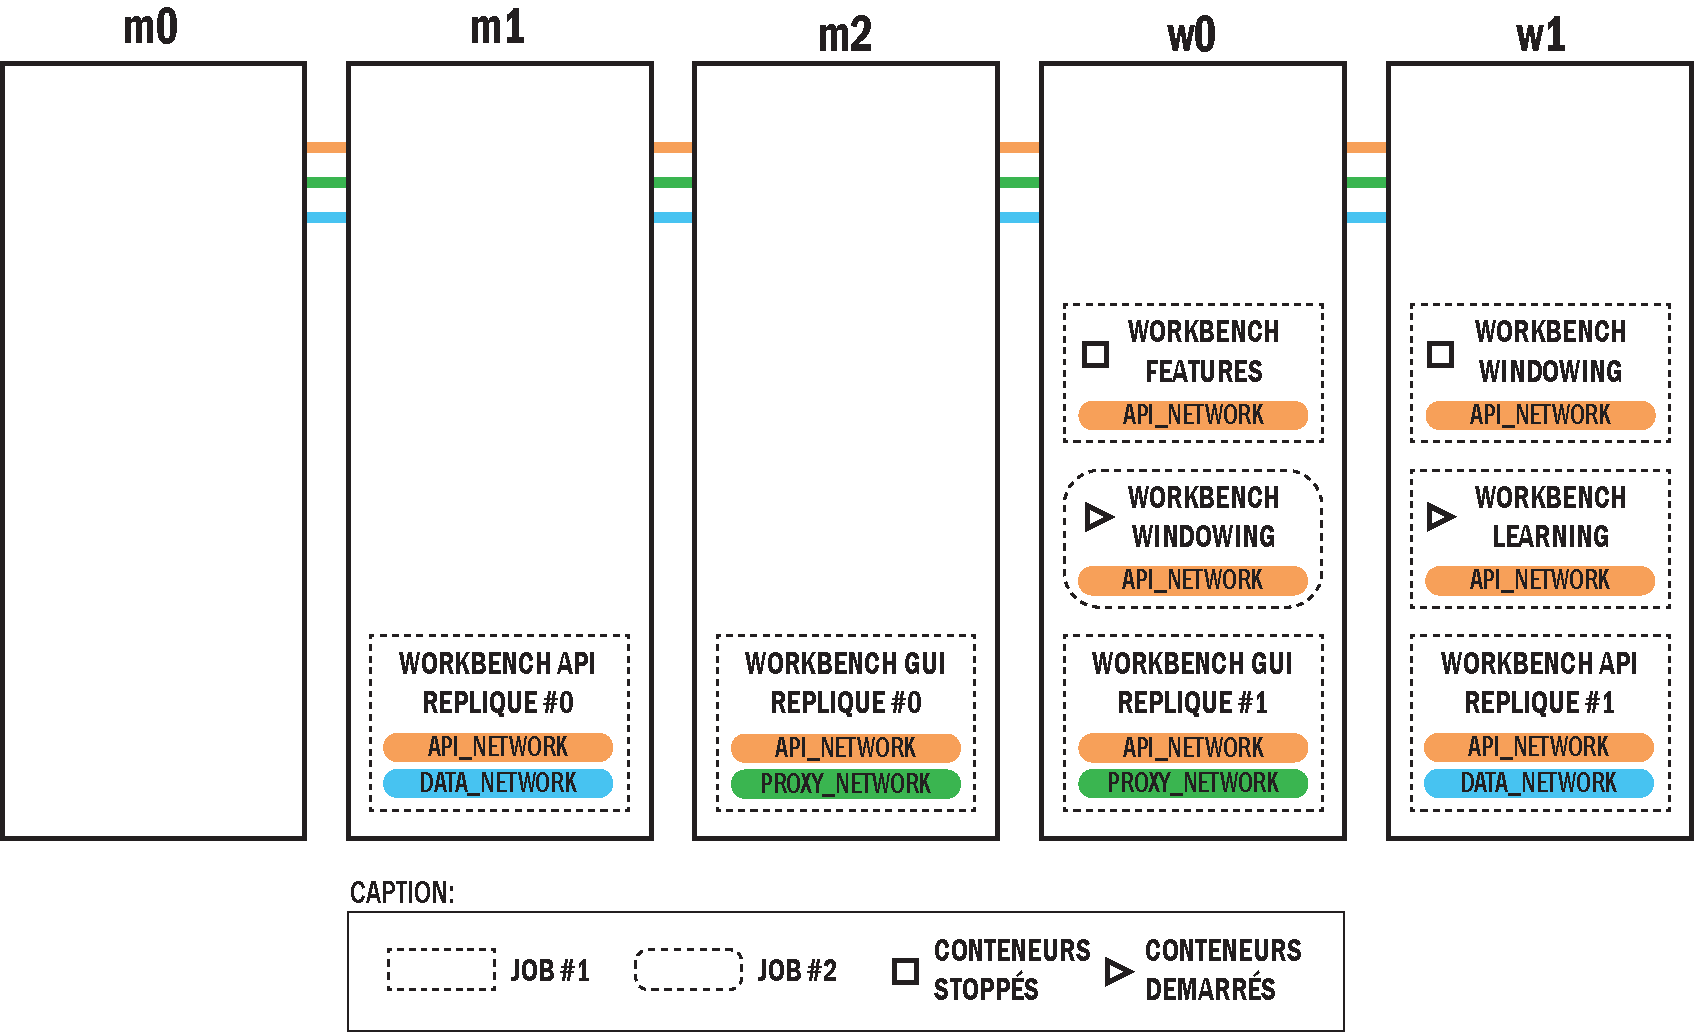
\includegraphics[width=.9\linewidth]{chapter6/containers_workbench.pdf}
        \caption{Exemple de placement des conteneurs et leurs réseaux superposés sur chaque n\oe{}ud de l'architecture proposée précédemment lors du déploiement de \acs{LE2ML}.}
	\label{fig:containers_workbench}
\end{figure}

\subsection{\acs{API} \acs{REST}}

En tant que composant logiciel principal dans la conception de \acs{LE2ML}, l'\acs{API}\footnote{\url{https://github.com/FlorentinTh/LE2ML-API}}, a été développée grâce à Node.js\footnote{\url{https://nodejs.org}}. Cet outil constitue un environnement d'exécution basée sur le moteur V8\footnote{\url{https://v8.dev}} qui permet de créer des applications côté serveur en JavaScript. Ensuite, le \textit{framework} Express.js\footnote{\url{https://expressjs.com}} a également été employé pour la création de l'\acs{API} \acs{REST}. Plus précisément, celui-ci a permis de simplifier la définition des fonctions de traitement associées aux requêtes \acs{HTTP} qui répondent aux différentes \acs{URI} de l'application (cf. Section \ref{sec:services_web}).

Par ailleurs, comme le montre la Figure \ref{fig:containers_workbench}, cette \acs{API} a été déployée en tant que service utilisant deux répliques. Celles-ci peuvent être exécutées soit sur des n\oe{}uds de type \textit{manager} ou sur des \textit{workers}. Cet exemple de déploiement demeure la recommandation suggérée puisque l'accessibilité de l'\acs{API} est garantie, même en cas de défaillance d'un n\oe{}ud de l'architecture. Toutefois, en fonction de la demande en ressource, c'est-à-dire, lorsque l'\acs{API} doit traiter un grand nombre de requêtes qui sont produites par plusieurs utilisateurs, il est possible de procéder à une mise à l'échelle du service afin d'éviter un ralentissement de l'ensemble du \textit{workbench}. De plus, bien que le service de l'\acs{API} fournisse son propre réseau superposé (\texttt{api\_network}), l'ensemble de ses répliques doivent aussi être relié au réseau de données (\texttt{data\_network}) afin de pouvoir communiquer avec la base de données déployée au sein de l'architecture. En effet, l'\acs{API} doit principalement être en mesure de manipuler les données relatives aux utilisateurs, tâches et sources de données, mais également aux algorithmes d'apprentissage machine, de fenêtrage et d'extraction de caractéristiques qui sont utilisés dans les modules de \acs{LE2ML}. Bien que cette implémentation a été préférée dans le cadre d'une utilisation avec l'architecture présentée dans le chapitre précédent, la mise à disposition d'une base de données non relationnelle n'est cependant pas une contrainte imposée pour assurer le fonctionnement du \textit{workbench} dans des environnements différents.

L'objectif principal de l'\acs{API} de \acs{LE2ML} est d'exécuter plusieurs processus (\emph{jobs}) d'apprentissage machine simultanés grâce à la définition de \textit{pipelines} pour ce processus. Pour ce faire, l'\acs{API} est chargée d'orchestrer le démarrage des différents modules du \textit{workbench} qui s'exécutent alors à l'intérieur de conteneurs. Lorsque tous les modules ont terminé, le \textit{pipeline} d'apprentissage machine est complété et la performance de la reconnaissance est donnée selon plusieurs métriques d'évaluation. De plus, l'\acs{API} propose également plusieurs fonctionnalités de base qui ne sont pas des modules, car elles sont complémentaires au processus d'apprentissage machine. Celles-ci comprennent l'importation de fichiers de données, la gestion de ces fichiers importés ou nouvellement créés, la visualisation des données, la gestion de l'authentification et des autorisations pour les utilisateurs et les applications, la gestion des utilisateurs et de leur rôle ainsi que la gestion des modules.

La définition d'un \textit{pipeline} d'apprentissage machine se fait par le biais d'un fichier \ac{YAML}. Cette approche a été choisie, car un tel type de fichier demeure plus facile à lire et à écrire que le format \acs{JSON}. Par ailleurs, le \acs{YAML} est un format qui se prête particulièrement bien avec l'utilisation de systèmes de gestion de versions (\aclp{VCS} ou \acsp{VCS}) pour être partagés entre plusieurs expérimentateurs au sein d'une équipe de recherche. Une fois transmis à l'\acs{API}, le fichier de définition du \textit{pipeline} est converti en format JSON afin d'être validé grâce à un schéma, puis il est stocké sur le système de fichiers distribué. Ensuite, le contenu du fichier est analysé par l'\acs{API} afin que toutes les tâches qui composent le \textit{pipeline} soient lancées de manière consécutive. Un exemple d'un tel fichier de définition est présenté en Figure \ref{fig:pipeline_conf}.

\begin{figure}[H]
	\centering
	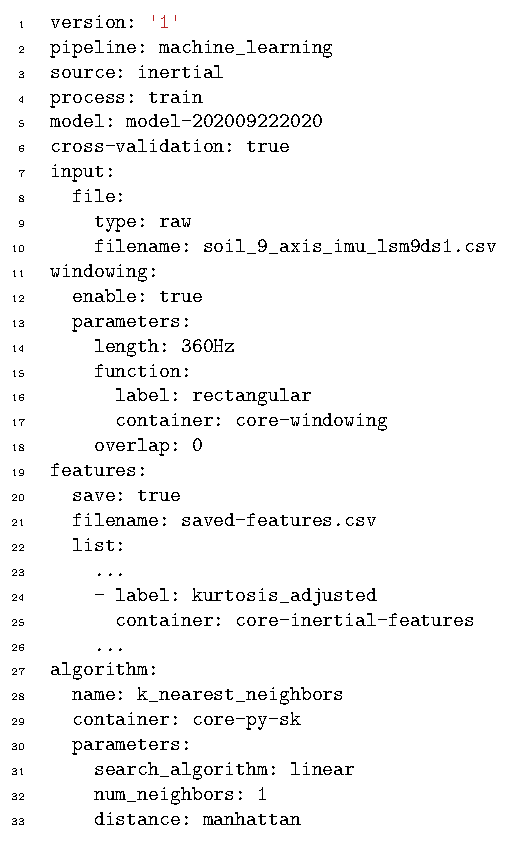
\includegraphics[width=.45\linewidth,keepaspectratio]{chapter6/pipeline_conf.pdf}
        \caption{Exemple d'un fichier de définition d'un \textit{pipeline} qui décrit la phase d'entraînement d'un processus d'apprentissage machine traditionnel.}
	\label{fig:pipeline_conf}
\end{figure}

Dans un premier temps, l'utilisateur doit préciser le type de \textit{pipeline} qui doit être réalisé. Les possibilités sont soit apprentissage machine (\texttt{machine\_learning}), soit apprentissage profond (\texttt{deep\_learning}). Une autre propriété obligatoire concerne la source de données. Celle-ci correspond au type de données qui sont traitées au cours du processus (\textit{p. ex.} des données inertielles ou vocales). Par ailleurs, lorsqu'il s'agit d'un \textit{pipeline} définissant un processus d'apprentissage machine traditionnel, la propriété \texttt{process} doit également être déclarée. Les valeurs possibles sont \texttt{train} et \texttt{test} qui font respectivement référence aux phases d'entraînement et de test pour un tel processus. Il est également possible d'y attribuer la valeur \texttt{none}\textemdash ceci dans le but de permettre aux utilisateurs de réaliser uniquement certaines tâches qui précèdent le processus d'apprentissage, comme l'extraction de caractéristiques. Comme le montre cet exemple, dans le cas où le \textit{pipeline} doit accomplir une phase d'entraînement, l'attribut \texttt{model} doit obligatoirement être fourni. Ainsi, le modèle de données qui a été entrainé par l'algorithme d'apprentissage est sauvegardé sur le système de fichier pour être réutilisé ultérieurement (\textit{p. ex.} lors de la définition d'une phase de prédiction). De plus, la propriété \texttt{cross-validation} est la dernière propriété imposée lorsqu'il s'agit d'une phase d'entraînement. Elle permet de produire une estimation des performances de reconnaissance en évaluant le modèle nouvellement créé grâce à la méthode de la validation croisée en 10 plis.

Ensuite, il est nécessaire de déclarer les données d'entrée sur lesquelles est appliqué le processus d'apprentissage machine. Actuellement, seules deux options sont autorisées, à savoir, la définition d'un fichier ou une connexion WebSocket. Lorsqu'il s'agit d'une source d'entrée de type WebSocket, l'\acs{URL} du serveur doit être indiquée. Sinon, les fichiers doivent être référencés selon leur nom et le type de données qu'ils contiennent (\textit{p. ex.} données brutes : \texttt{raw}). Enfin, le reste du contenu du fichier permet de décrire les différentes tâches et leurs paramètres associés qui sont utilisés lors de l'exécution des modules.

Pour compléter l'exécution des \emph{jobs}, l'\acs{API} a la responsabilité de démarrer les conteneurs selon la définition des tâches fournie dans les fichiers de définition de \textit{pipelines}. Ainsi, puisque certains conteneurs dépendent du résultat de la tâche précédente, ils sont, pour un \emph{job} donné, lancés les uns après les autres. Néanmoins, lorsqu'une même tâche est définie pour utiliser plusieurs conteneurs distincts, ceux-ci sont démarrés en même temps. Ils s'exécutent alors en parallèle. Enfin, les \emph{jobs} qui sont créés par les différents utilisateurs du \textit{workbench} sont également exécutés en parallèle. Ceux-ci sont aussi indépendants les uns des autres bien qu'ils utilisent des images de conteneurs identiques. À titre d'exemple, la Figure \ref{fig:containers_workbench} montre deux \emph{jobs} démarrés à des moments différents, mais dont le traitement est concurrent. En effet, il est possible d'observer que pour le premier \emph{job}, les tâches de fenêtrage et d'extraction de caractéristiques sont toutes les deux terminées alors que le conteneur d'apprentissage est toujours en cours d'exécution. À l'inverse, la tâche de fenêtrage pour le second \emph{job} vient juste de commencer et les autres conteneurs ne sont pas visibles, car ils n'ont pas encore été démarrés.

Pour qu'un conteneur devienne un module de \acs{LE2ML}, trois variables d'environnement doivent être définies, lors de son lancement. Il s'agit de l'identifiant unique du \emph{travail}, de l'identifiant unique de l'utilisateur ainsi que d'un jeton unique généré aléatoirement pour chaque conteneur. Le jeton est utilisé pour permettre à l'\acs{API} de faire le lien entre un conteneur en particulier et la tâche à laquelle il est rattaché. Par conséquent, il est possible de mettre à jour l'entrée du \emph{job} associé dans la base de données. En effet, une fois son traitement terminé, un module LE2ML doit communiquer son état (succès ou échec) à l'\acs{API} par le biais d'un \textit{endpoint} prévu à cet effet. De telles requêtes ne sont permises que si les conteneurs y sont autorisés. Cette vérification est établie grâce à une clé d'application générée au préalable pour chaque application.

Finalement, comme l'exécution des processus d'apprentissage machine implique la création de fichiers, ces informations résultantes du traitement de chaque tâche du \textit{pipeline} sont écrites sur le système dans des dossiers séparés par \emph{job}. En ce sens, ces dossiers sont montés en tant qu'espaces de travail pour tous les conteneurs définis pour un \emph{job} donné.

\subsection{Application Web}

Pour faciliter l'interaction avec l'\acs{API}, nous avons jugé approprié de proposer une interface. De ce fait, une interface graphique\footnote{\url{https://github.com/FlorentinTh/LE2ML-GUI}} a été préférée à une interface de type \acs{CLI} (dont le développement n'est pas exclu dans un avenir proche). En effet, puisque les équipes de recherche sont, la plupart du temps, multidisciplinaires, la conception d'une \acs{GUI} a été priorisée, car ce type d'interface est plus simple à apprendre et à utiliser pour les utilisateurs néophytes. Cette application web a été développée grâce à des technologies modernes. En effet, sa conception repose principalement sur un \textit{framework} JavaScript qui supporte ECMAScript 6 et les versions supérieures de ce standard (ES6+). Celui-ci a été développé spécifiquement pour les besoins de cette application. Par ailleurs, la stratégie de déploiement qui a été adoptée pour ce composant applicatif demeure la même que pour l'\acs{API}, c'est-à-dire, un service répliqué admettant deux instances qui peuvent être placées soit sur un n\oe{}ud \textit{manager}, soit sur un \textit{worker}.

La Figure \ref{fig:le2ml_gui} montre une capture d'écran de la vue principale de l'interface qui permet de créer des \textit{jobs} d'apprentissage machine. Le fil d'Ariane (\texttt{A}) permet d'indiquer aux utilisateurs les étapes qui doivent être complétées pour définir toutes les tâches du \textit{pipeline}. Dans une vue précédente à cette capture d'écran, l'utilisateur doit sélectionner le type d'apprentissage machine qu'il souhaite réaliser (dans le cas présent, il s'agit d'un apprentissage machine traditionnel). Pour chaque étape du \textit{pipeline}, un ensemble de composants web (\texttt{B}) est proposé pour permettre aux utilisateurs de configurer chaque tâche de manière pratique. Cependant, bien qu'il soit possible de construire les fichiers de définition en interagissant avec l'interface graphique, une fonction d'import (\texttt{C}) a également été prévue pour permettre la réutilisation des définitions de \textit{pipeline} existantes. Dans ce contexte, les composants web pour chacune des étapes sont préremplis en fonction du contenu du fichier téléchargé.

\begin{figure}[H]
	\centering
	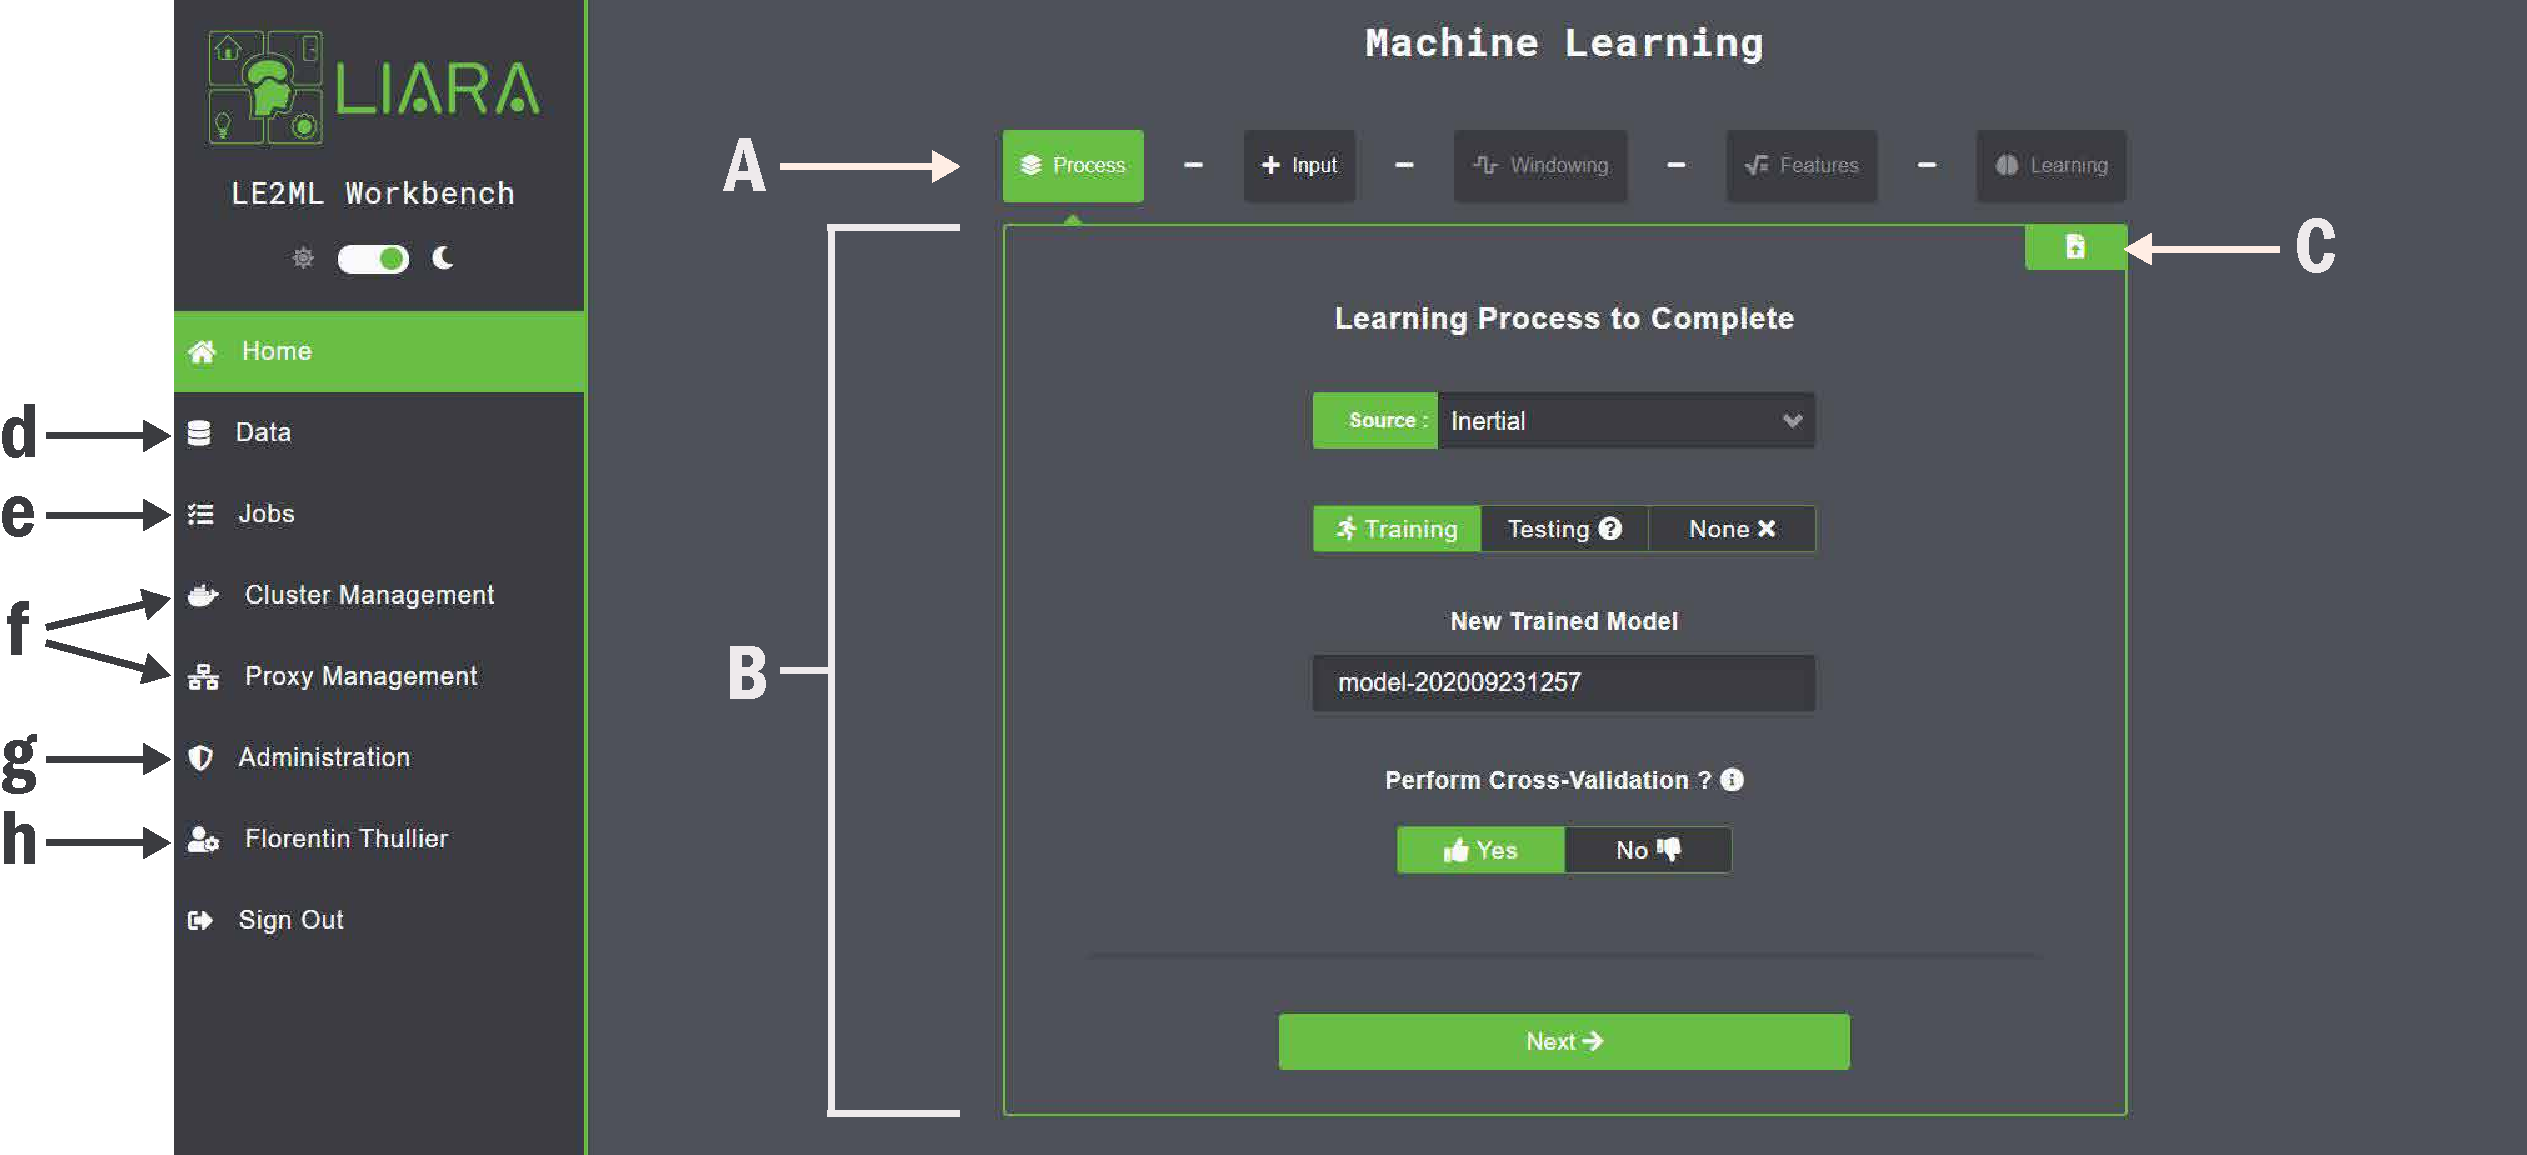
\includegraphics[angle=90,origin=c,height=.85\textwidth,keepaspectratio]{chapter6/le2ml_gui.pdf}
        \caption{Capture d'écran de l'application web qui montre la première étape de la définition d'un \textit{pipeline} d'apprentissage machine.}
	\label{fig:le2ml_gui}
\end{figure}

Par ailleurs, cette interface offre également aux utilisateurs un moyen d'interagir avec toutes les autres fonctionnalités de l'\acs{API}. Le menu \textit{Data} (\texttt{d}) regroupe toutes les fonctionnalités liées aux fichiers de données d'entrée. Celles-ci comprennent un composant pour téléverser de nouveaux fichiers, une vue permettant de naviguer dans le système de fichiers distribué, un outil de visualisation des données ainsi qu'un accès aux différents modules de prétraitement et de fusion des données. Le menu \textit{Jobs} (\texttt{e}) présente la liste des \textit{jobs} d'apprentissage machine en cours de traitement et terminés qui ont été créés par l'utilisateur connecté. Cette liste est mise à jour en temps réel grâce à la technologie \ac{SSE} qui permet à l'\acs{API} d'envoyer des notifications \textit{push} à l'application web. Par le biais de cette vue, il est également possible de télécharger les fichiers résultant d'un \textit{job} complété. Ces fichiers peuvent être soit un rapport comprenant des mesures d'évaluation de la performance qui sont calculées pendant la phase d'entraînement, soit la liste des prédictions déterminées lors de la phase de test. Ensuite, les menus \textit{Cluster Management} et \textit{Proxy Management} (\texttt{f}) redirigent vers les tableaux de bord de Portainer et de Tr\ae{}fik respectivement. Le menu \textit{Administration} (\texttt{g}) permet aux utilisateurs qui ont le rôle administrateur de gérer les modules, les clés d'application ainsi que les utilisateurs inscrits. Enfin, les utilisateurs connectés ont également accès à leur profil (\texttt{i}), où il leur est possible de modifier la plupart de leurs informations personnelles, y compris leur mot de passe.

\subsection{Modules proposés}

Dans la mesure où \acs{LE2ML}, de par sa conception, a pour objectif de fournir une meilleure flexibilité, plusieurs modules ont été conçus pour réaliser certaines tâches spécifiques qui composent le processus d'apprentissage machine. Leur développement a été simplifié afin que quiconque soit capable d'étendre les fonctionnalités du \textit{workbench} en proposant ses propres mécanismes. Ainsi, il est possible de proposer des modules pour le traitement de données telles que les méthodes de prétraitement ou de fusion de données, mais également, des modules qui proposent de nouvelles techniques d'extraction de caractéristiques ou de nouveaux algorithmes d'apprentissage machine.

Le premier avantage principal qui motive l'usage de modules est qu'ils fournissent un moyen simple de pallier la diversité dans la conception de logiciels, tant en termes de langages de programmation, que d'environnements d'exécution qui forment le vaste monde des techniques liées au processus d'apprentissage machine. Par exemple, lorsque des chercheurs développent de nouveaux algorithmes, ces derniers ne devraient pas avoir à se préoccuper de la compatibilité de leur nouvelle implémentation avec un environnement existant. Ainsi, grâce à un outil modulaire, qui demeure agnostique et flexible, ils ont la possibilité d'évaluer les performances de leur méthode en utilisant la technologie qu'ils jugent la plus appropriée, tout en bénéficiant de la puissance des outils dont elle dispose (\textit{p. ex.} librairies, \textit{framework}, \textit{etc.}). Le deuxième avantage à l'utilisation de modules est qu'ils facilitent considérablement l'exécution en parallèle et la mise à l'échelle de nombreux processus, puisque ceux-ci s'exécutent au sein de conteneurs. Bien qu'il soit possible d'imaginer une quantité infinie de modules, cette section n'en décrit que trois qui ont été développés spécifiquement pour répondre aux besoins de notre laboratoire. Plus précisément, ces modules doivent permettre la réplication de la méthode de reconnaissance des types de sols proposée au Chapitre \ref{chap:4}.

\subsubsection{Fenêtrage}

Nous avons vu que le processus d'apprentissage machine peut impliquer l'utilisation de signaux ou de séries temporelles comme données d'entrée. Par conséquent, il est parfois nécessaire d'appliquer une fonction de fenêtre glissante pour segmenter ces données brutes en de plus petits ensembles. En ce sens, puisque plusieurs travaux proposés par notre laboratoire de recherche se sont basés sur l'exploitation de telles données \citep{Thullier2017,Chapron2018,Bouchard2020}, nous avons décidé de fournir un module de fenêtrage pour \acs{LE2ML}\footnote{\url{https://github.com/FlorentinTh/LE2ML-Windowing-Module}}. Développé en JavaScript \texttt{ES6+}, ce module propose les fonctions de fenêtrage les plus connues qui sont généralement appliquées sur ce type de données, c'est-à-dire les fonctions rectangulaires, triangulaires, de Hamming (cf. Équation \ref{eq:hamming}), de Hann (cf. Équation \ref{eq:hann}) et de Blackmann (cf. Équation \ref{eq:blackman}). En outre, ce module permet également de configurer plusieurs autres paramètres dont ce processus de segmentation dépend, comme la taille de la fenêtre glissante (cf. ligne 14 de la Figure \ref{fig:pipeline_conf}). Ce paramètre s'exprime dans différentes unités selon que les données admettent un horodatage (\textit{timestamp}) ou non. Par exemple, si les données ne sont pas horodatées, la taille de la fenêtre peut être donnée en fonction d'une unité de fréquence (\textit{p. ex.} Hz), sinon une unité de temps (\textit{p. ex.} secondes ou minutes) peut être préférée. De plus, il est également possible de définir un paramètre de chevauchement qui est alors exprimé en pourcentage de la taille de la fenêtre (cf. ligne 18 de la Figure \ref{fig:pipeline_conf}). Enfin, dans le but de garantir la meilleure efficacité possible, tant en termes d'utilisation des ressources de calcul que de consommation mémoire, l'implémentation de ce module repose principalement sur un traitement des données en flux (\textit{streams}), qui a été mis en place grâce à l'environnement Node.js.

\subsubsection{Extraction de caractéristiques}

L'extraction de caractéristiques demeure une tâche importante à accomplir dans le traitement du processus d'apprentissage machine. Pour rappel, l'objectif d'une telle tâche est de calculer des vecteurs de caractéristiques discriminantes basés sur chacun des segments de données brutes obtenus à partir du processus de fenêtrage précédent. En ce sens, puisque plusieurs recherches menées au sein de notre laboratoire ont utilisé des centrales inertielles (\acsp{IMU}) \citep{Thullier2017,Thullier2018,Chapron2018}, un module qui propose les principales caractéristiques qu'il est possible d'obtenir grâce à ce type de données a été développé\footnote{\url{https://github.com/FlorentinTh/LE2ML-FeatureExtractor-Module}}. De ce fait, onze caractéristiques différentes provenant des domaines temporel et fréquentiel peuvent être calculées. Celles-ci incluent l'asymétrie (cf. Équation \ref{eq:asymetrie}), l'aplatissement (cf. Équation \ref{eq:kurtosis}), la composante continue, l'énergie spectrale (cf. Équation \ref{eq:energy_spec}) et l'entropie (cf. Équation \ref{eq:entropy}). Par ailleurs, ce module a également été développé en JavaScript \texttt{ES6+}. Cependant, bien que ce langage ne soit pas fortement typé et ne semble pas adapté au calcul de formules mathématiques complexes, une précision et des performances identiques ont été observées par rapport au programme écrit en Go\footnote{\url{https://github.com/LIARALab/GoLang-FeatureExtractor}} utilisé dans la méthode proposée dans le Chapitre \ref{chap:4}. En effet, de la même manière que pour le module de fenêtrage, une attention particulière a été portée sur l'efficacité de la consommation de la mémoire lors du développement de ce module, notamment grâce au traitement des fichiers par flux de données. Enfin, cette implémentation se veut également flexible quant au type de signal qu'il reçoit en entrée, car celui-ci s'appuie sur l'utilisation de l'algorithme de la \acs{FFT} de Bluestein \citep{Bluestein1970} pour le passage du domaine temporel au domaine fréquentiel.

La première version des fichiers de définition pour les \textit{pipelines} d'apprentissage machine permet, dans un premier temps, de lister un ensemble de caractéristiques à extraire sur des données brutes fournies en entrée (cf. ligne 22 de la Figure \ref{fig:pipeline_conf}). Cette liste est soit vide, soit elle contient des objets qui définissent chacune des caractéristiques. Ceux-ci sont composés du libellé et du nom du conteneur (l'environnement d'exécution du module) qui est utilisé pour son calcul. Lorsque cette liste est vide, le processus d'extraction des caractéristiques n'est pas réalisé. Néanmoins, lorsque la liste contient des caractéristiques, leurs définitions peuvent inclure des conteneurs différents. Ainsi, il est possible d'exploiter plusieurs modules de ce type pour compléter le processus d'extraction de caractéristiques sur un même signal. Par conséquent, chaque module est responsable du traitement des caractéristiques qui lui sont associées. Les conteneurs s'exécutent donc en parallèle et ils sont indépendants les uns des autres. De ce fait, la tâche est complétée lorsque le dernier conteneur termine son exécution. Son état est alors mis à jour dans la base de données et une opération de fusion est déclenchée par l'\acs{API}. Celle-ci permet alors d'assembler chacun des fichiers qui ont été produits par les conteneurs afin qu'un seul fichier résultant soit fourni comme entrée à l'algorithme d'apprentissage machine.

\subsubsection{Apprentissage machine}

Le module d'apprentissage machine proposé\footnote{\url{https://github.com/FlorentinTh/LE2ML-Learning-Module}} pour cette première version du \textit{workbench} a été conçu pour permettre l'utilisation d'algorithmes d'apprentissage machine traditionnels uniquement. Celui-ci a été développé en Python 3, car sa conception constitue une surcouche logicielle de la librairie scikit-learn qui est également développée en Python. Ainsi, l'objectif de ce module est de traduire automatiquement les paramètres des fichiers de configuration de \textit{pipelines} (cf. ligne 30 de la Figure \ref{fig:pipeline_conf}) en code compatible avec l'\acs{API} de cette librairie. En ce sens, il est possible, dans un premier temps, d'entraîner des modèles grâce à plusieurs algorithmes qui sont définis dans la surcouche, comme \acl{KNN} et \textit{random forest}. Ensuite, une évaluation pour cette phase d'entraînement peut être réalisée grâce à la méthode de la validation croisée en 10-plis. Par conséquent, une matrice de confusion ainsi que des mesures pertinentes telles que la justesse, la $F\mbox{-} mesure$ et la Kappa de Cohen peuvent être fournies, une fois le \textit{pipeline} complété. Dans un second temps, puisque ce module d'apprentissage machine permet de sauvegarder les modèles d'apprentissage sur le système de fichier distribué, ceux-ci peuvent être réutilisés lors de la phase de reconnaissance afin de produire un ensemble de prédictions. Par ailleurs, les phases d'entraînement et de reconnaissance ont été explicitement configurées pour exploiter, de manière automatique, toutes les ressources disponibles allouées aux conteneurs de ce module.

% \subsection{Réutilisation des modules}


\section{Expérimentations \& Résultats}

Cette section présente une expérimentation qui a été réalisée afin de montrer les capacités non limitatives du \textit{workbench} pour une utilisation académique des \textit{wearable devices} au sein des habitats intelligents. Ainsi, grâce à \acs{LE2ML}, nous avons été en mesure de reproduire le processus d'apprentissage de la méthode de reconnaissance des types de sols qui a été proposée au Chapitre \ref{chap:4}. Pour ce faire, aucun code n'a dû être réécrit ou adapté\textemdash seul un fichier de définition de \textit{pipeline} accompagné des données brutes récoltées précédemment ont été nécessaires. En ce sens, ce sont les données produites par l'\acs{IMU} 9-axes du \textit{wearable device} qui ont été utilisées. De plus, afin de respecter la méthode qui a été proposée, deux \textit{jobs} distincts ont été créés \textit{via} le \textit{workbench}, chacun correspondant à une définition spécifique pour les différents algorithmes d'apprentissage. La première concerne l'algorithme \acs{KNN} configuré avec les paramètres qui ont été identifiés comme optimaux c'est-à-dire, $k=1$ voisin et une recherche linéaire de celui-ci grâce au calcul de la mesure de distance de Manhattan ($D_m$). Par ailleurs, la seconde configuration a permis de spécifier les paramètres pour l'algorithme \textit{random forest} soit, $B=300$ arbres, $F=\lfloor\log_2(m) + 1\rfloor$ variables aléatoires et l'évaluation du gain en information selon l'entropie de Shannon. De la même manière que dans le Chapitre \ref{chap:4}, l'évaluation de la performance a été réalisée grâce à la validation croisée en 10 plis. Les résultats qui ont été obtenus pour cette expérimentation sont présentés dans le Tableau \ref{tab:results_workbench}.

\begin{table}[H]
  \centering
  \caption{Évaluations des performances de la reconnaissance des types de sols sur des données inertielles obtenues respectivement avec la méthode originelle et avec \acs{LE2ML}.}
  \label{tab:results_workbench}
  \begin{tabular}{@{}rccc@{}}
    \toprule
      \multicolumn{4}{c}{\textbf{Méthode Originelle}} \\
    \midrule
      \multicolumn{1}{l}{} & \textit{Justesse} & $F\mbox{-} mesure$ & \textit{Kappa de Cohen} \\[-10pt]
      \textbf{$k$-NN} & 0.93 & 0.93 & 0.89 \\[-10pt]
      \textbf{\textit{Random Forest}} & 0.92 & 0.92 & 0.88 \\
    \bottomrule
  \end{tabular}
  \begin{tabular}{@{}rccc@{}}
      \multicolumn{4}{c}{\textbf{\textit{Pieplines} \acs{LE2ML}}} \\
    \midrule
      \multicolumn{1}{l}{} & \textit{Justesse} & $F\mbox{-} mesure$ & \textit{Kappa de Cohen} \\[-10pt]
      \textbf{$k$-NN} & 0.91 & 0.91 & 0.86 \\[-10pt]
      \textbf{\textit{Random Forest}} & 0.92 & 0.92 & 0.88 \\
    \bottomrule
  \end{tabular}
\end{table}

En ce qui concerne ces résultats, il nous est possible d'affirmer que notre \textit{workbench} offre un niveau de précision similaire à celui de \acs{WEKA}. En effet, les performances de reconnaissance qui ont été obtenues dans les deux cas demeurent pratiquement identiques, et ce, pour les trois métriques d'évaluation. Néanmoins, le faible écart observé avec l'algorithme \acs{KNN} n'est pas assez significatif et peut s'expliquer simplement par les différences qui résident dans l'implémentation des deux outils.

\section{Conclusion}

Dans ce chapitre, un nouveau type de \textit{workbench} d'apprentissage machine appelé \ac{LE2ML} a été présenté. Grâce à une conception modulaire qui repose sur l'utilisation de microservices, cet outil a été \hl{avant tout} prévu pour fonctionner au sein de l'architecture distribuée introduite au chapitre précédent. Toutefois, il est également possible que ce \textit{workbench} soit utilisé dans des environnements différents qui admettent, par exemple, une architecture monolithique plus conventionnelle. L'implémentation de \acs{LE2ML} repose sur une \acs{API} \acs{REST}. Cette dernière représente le composant principal du \textit{workbench} puisqu'elle est responsable de l'orchestration de l'ensemble du système et plus particulièrement des modules. Afin de répondre aux besoins exprimés par la définition du processus d'apprentissage, ces modules peuvent être soit réutilisés, soit développés spécifiquement. Ainsi, puisque plusieurs recherches réalisées au \acs{LIARA} se sont basées sur l'exploitation d'\acsp{IMU} embarqués dans des \textit{wearable devices}, tous les modules qui ont été présentés dans ce chapitre ont été principalement conçus pour traiter ce type de données, à l'exception du module d'apprentissage machine.

De plus, pour interagir avec l'\acs{API}, une interface web a été développée, essentiellement pour simplifier la création de fichiers de définition de pipeline qui décrivent l'ensemble du processus d'apprentissage de la machine à réaliser. \hl{Ce fichier de définition demeure un élément important du système puisqu'il permet à l'API de piloter des composants logiciels hétérogènes qui font que} \acs{LE2ML} \hl{est un \textit{workbench} et agnostique vis-à-vis des technologies. À titre d'exemple, une telle flexibilité a pu être démontrée grâce au \textit{pipeline} d'exemple qui a fait intervenir plusieurs composants développés en JavaScript et en Go, et ce, sans avoir à écrire de code.}

Enfin, une des expérimentations réalisées dans le Chapitre \ref{chap:4} a été reproduite \textit{via} ce \textit{workbench}. Les résultats qui ont été obtenus n'ont pas montré de différences significatives en ce qui concerne la performance de reconnaissance par rapport à ceux de la méthode précédente. Par conséquent, malgré un nombre encore limité de modules disponibles, nous pensons que \acs{LE2ML} demeure un outil indispensable pour favoriser l'intégration des \textit{wearable devices} dans les habitats intelligents en milieu académique\hl{\textemdash étant donné que cet outil permet de faire le lien entre la couche matérielle offerte par l'architecture et les composants logiciels qui sont développés à la fois pour les \textit{wearable devices}, mais également pour les capteurs ambiants.}

\let\cleardoublepage\clearpage
\begin{conclusion}

\end{conclusion}
\let\cleardoublepage\clearpage

%%%%%%%%%%%%%
%% Références
%%%%%%%%%%%%%

\bibliographystyle{apa-uqac}
\bibliography{assets/references}

%%%%%%%%%%%%
%% Annexes
%%%%%%%%%%%%
\appendix

\chapter{Première Annexe}


\end{document}
